\documentclass[
  reprint,
  amsmath,
  amssymb,
  aps,
  pra,
  nofootinbib,
  superscriptaddress,
  floatfix
]{revtex4-2}
\usepackage[T1]{fontenc}
\usepackage{lmodern}
\usepackage{newunicodechar}
\newunicodechar{’}{'}
\usepackage{graphicx}
\graphicspath{{../../}{}}
\usepackage{capt-of} % \captionof for non-floating figures (used with widetext)
\usepackage{booktabs}
\usepackage{bm}
\usepackage{mathtools}
\usepackage{amsthm}
\usepackage{xcolor}
\usepackage{hyperref}
\hypersetup{hidelinks}

\newcommand{\placeholder}[1]{\textcolor{red!70!black}{\ifmmode\left[#1\right]\else\textsf{[#1]}\fi}}
\newcommand{\tentative}[1]{\textcolor{red!70!black}{#1}}
\newcommand{\structlabel}[1]{\noindent\mbox{\tentative{#1.}}~}
\newcommand{\Oset}{\mathcal{O}}
\newcommand{\Gset}{\mathcal{G}}
\newcommand{\Rset}{\mathcal{R}}
\newcommand{\Sset}{\mathcal{S}}
\newcommand{\Hcal}{\mathcal{H}}
\newcommand{\Bcal}{\mathcal{B}}
\newcommand{\Ocal}{\mathcal{O}}
\newcommand{\Ucal}{\mathcal{U}}
\newcommand{\Jcal}{\mathcal{J}}
\newcommand{\Pcal}{\mathcal{P}}
\newcommand{\Dcal}{\mathcal{D}}
\newcommand{\Wcal}{\mathcal{W}}
\newcommand{\dd}{\mathrm{d}}
\newcommand{\ii}{\mathrm{i}}
\newcommand{\ee}{\mathrm{e}}
\newcommand{\TR}{\mathrm{TR}}
\newcommand{\ex}{\mathrm{ex}}
\newcommand{\ctrl}{\mathrm{ctrl}}
\newcommand{\stat}{\mathrm{stat}}
\newcommand{\dyn}{\mathrm{dyn}}
\newcommand{\drv}{\mathrm{drv}}
\newcommand{\obs}{\mathrm{obs}}
\newcommand{\stay}{\mathrm{stay}}
\newcommand{\app}{\mathrm{append}}
\newcommand{\ablate}{\mathrm{ablate}}
\newcommand{\Var}{\operatorname{Var}}
\newcommand{\Tr}{\operatorname{Tr}}
\newcommand{\Top}{\operatorname{Top}}
\newcommand{\argminp}{\mathop{\mathrm{arg\,min}}}
\newcommand{\argmaxp}{\mathop{\mathrm{arg\,max}}}
\newcommand{\proj}{\mathrm{proj}}
\newcommand{\diag}{\mathrm{diag}}
\newcommand{\CVaR}{\operatorname{CVaR}}
\newcommand{\softmax}{\operatorname{softmax}}
\newcommand{\hh}{\mathrm{HH}}
\newcommand{\phmax}{n_{\mathrm{ph,max}}}
\newcommand{\twq}{\mathrm{2Q}}
\newcommand{\eps}{\varepsilon}
\newcommand{\ket}[1]{|#1\rangle}
\newcommand{\bra}[1]{\langle #1|}
\newcommand{\braket}[2]{\langle #1|#2\rangle}
\newcommand{\expval}[1]{\langle #1\rangle}
\newcommand{\metrichead}[1]{\makebox[0.061\textwidth][c]{#1}}
\newcommand{\archmetrichead}[1]{\makebox[0.040\textwidth][c]{#1}}
\newcommand{\inlinetablecaption}[2]{%
  \par\addvspace{1.6ex}%
  \captionof{table}{#2\label{#1}}%
  \par\addvspace{0.8ex}%
}
\newenvironment{schurlemma}[1][]
{\par\medskip\noindent\textbf{Lemma}\if\relax\detokenize{#1}\relax\else\ (#1)\fi.\space\itshape}
{\par\medskip}
\newenvironment{schurassumption}[1][]
{\par\medskip\noindent\textbf{Assumption}\if\relax\detokenize{#1}\relax\else\ (#1)\fi.\space}
{\par\medskip}
\newenvironment{schurtheorem}[1][]
{\par\medskip\noindent\textbf{Theorem}\if\relax\detokenize{#1}\relax\else\ (#1)\fi.\space\itshape}
{\par\medskip}
\newenvironment{schurremark}[1][]
{\par\medskip\noindent\textbf{Remark}\if\relax\detokenize{#1}\relax\else\ (#1)\fi.\space}
{\par\medskip}


\begin{document}

\makeatletter
\def\bibsection{\section*{\refname}\@nobreaktrue}
\makeatother

\title{Geometric and Resource-Aware Adaptive Ansatz Construction for Fermion--Boson Hamiltonian Systems}

\author{Jake Strobel}
\author{Jacopo Simoni}
\author{Gabriele Riva}
\author{Yuan Ping}
\affiliation{University of Wisconsin--Madison}

\date{\today}

\begin{abstract}
Near-term ground-state quantum simulation requires ansätze that must simultaneously satisfy expressivity while minimizing circuit depth, entangling gates, and measurement overhead. ADAPT-VQE addresses this problem; however, its gate-selection mechanism is sensitive to parameter heterogeneities, local gradient plateaus, state-tangent redundancy, and is agnostic to generator-specific hardware costs. We introduce SNAKE, which leverages a shortlisting mechanism to rank generators according to a joint triple objective: novel state-space displacement via a Fubini--Study metric least-squares treatment, a second-order, trust-region constrained energy model coupling the candidate generator's gradient to the existing ansatz via Schur reduction, and a graph-aware, generator-variance-competition model penalizing inordinate hardware costs. We present results of SNAKE, append-only ADAPT-VQE, and Geo-ADAPT tested on the Hubbard, spin-boson/Rabi, and Hubbard--Holstein using matched encodings, inner-optimization protocol, and operator-pool expressivity. Against ADAPT-VQE under the same operator-pool constraints, SNAKE attains lower energy error in five of six Hubbard--Holstein interaction regimes and lower compiled circuit burden in all six, with lower quantum-estimator queries in four of six. In the strong--strong regime, SNAKE has \(29.5\%\) higher energy error than ADAPT-VQE \((1.07\times10^{-5}\) natural energy units), but lowers the ADAPT-VQE resource burden by \(99.4\%\) in two-qubit gate count \((7{,}928)\), \(99.5\%\) in two-qubit depth \((7{,}794)\), and \(99.3\%\) in compiled depth \((26{,}031)\). These results show promise for accurate near-term quantum-chemistry applications on fermionic and mixed fermion--boson systems.


\end{abstract}

\maketitle







\section{Introduction}

Quantum processors can offer computational speedups in second-quantized Hamiltonian simulation problems \cite{Lloyd1996,AspuruGuzik2005}. The practical scope of near-term quantum simulation is constrained by hardware resources, where circuit-depth, entangling gate-count, and measurement overhead limit the Hilbert-space dimension capable of being effectively simulated due to the generally monotonic relationship of circuit-cost and observable noise \cite{Preskill2018NISQ,Cerezo2021VQA,Huggins2021Measurements}. This current state of hardware is classified as the noisy intermediate-scale quantum (NISQ) era. Variational quantum eigensolvers (VQE) are the near-term quantum-processor-compatible algorithmic class whose success depends on parameterized ansatz construction that must satisfactorily express the physical system while minimizing hardware-induced errors. Adaptive derivative-assembled pseudo-Trotter VQE (ADAPT-VQE) methods are a NISQ-friendly improvement over conventional VQE due to their ability to create compact circuits through a gradient-based operator-selection mechanism, though their measurement overhead can remain prohibitive and deficits in ansatz expressivity due to selection issues remain well-observed \cite{Grimsley2019,Tang2021,Yordanov2021,Feniou2023,Ramoa2025HessianRecycling,Ikhtiarudin2025ShotEfficient}. Ansatz construction through operator selection then becomes the mechanism either permitting or restricting quantum simulation. We present the variational adaptive algorithm, SNAKE, to address this bottleneck.


\subsubsection{Modeled problem}
To our knowledge, no ADAPT-VQE method has been applied to condensed-matter many-body fermion--phonon Hamiltonians such as the Hubbard--Holstein model \cite{Macridin2018,Li2023,Denner2023,Majland2024vADAPT}. Fermionic electronic-structure ADAPT can draw on a mature unitary coupled cluster single-double excitation (UCCSD) operator literature \cite{Romero2018UCC,Grimsley2019}, while no comparably established operator-pool construction exists for mixed fermion--phonon condensed-matter models. In the Hubbard--Holstein setting, the pool must span electronic correlation, phononic lattice response, and coupled electron--phonon dressing, with the encoded ansatz requiring fermion--boson sector-entangling gates under finite phonon-mode truncation \cite{Hubbard1963,Holstein1959a,Holstein1959b}. Section~\ref{subsec:hh_physical_operator_lanes} gives the corresponding Hamiltonian-local operator pool. We focus results on the Hubbard--Holstein model and compare append-only ADAPT-VQE, Geo-ADAPT, and SNAKE by energy error, fidelity error, and final circuit cost.


The Hubbard--Holstein model is given by
\begin{align}
H
&=-t\sum_{\langle i,j\rangle,\sigma}
(c_{i\sigma}^{\dagger}c_{j\sigma}+c_{j\sigma}^{\dagger}c_{i\sigma})
+U\sum_i n_{i\uparrow}n_{i\downarrow}
\nonumber\\
&\quad+\omega_0\sum_i b_i^\dagger b_i
+g\sum_i(b_i^\dagger+b_i)(n_i-\bar n).
\label{eq:hubbard_holstein_static}
\end{align}
Here \(c_{i\sigma}\) and \(b_i\) correspond to fermionic and bosonic annihilation operators, respectively, acting on site $i$, with creation given by $\dagger$; $\sigma \in\{\uparrow, \downarrow\}$ denotes particle spin;
\(n_{i\sigma}, n_i\) are the spin-resolved and total fermionic number operators, respectively; \(\bar n=N_e/L\) is the mean fermion filling
for fixed electron number \(N_e\) and lattice size \(L\). Our results use open boundary conditions with half-filling.
Here \(t\) is the nearest-neighbor electronic hopping amplitude, \(U\) is the onsite Hubbard interaction, \(\omega_0\) is the phonon frequency, \(g\) is the local electron--phonon coupling, and \(\langle i,j\rangle\) denotes nearest-neighbor lattice sites.
In the joint decoupling limit $g\to0$ and $\omega_0\to0$, the electronic sector reduces to the Hubbard Hamiltonian, up to a decoupled zero-frequency phonon register. We use Jordan--Wigner and binary encoding for Eq.~\eqref{eq:hubbard_holstein_static} and for the operator-pool generators in Sec.~\ref{subsec:hh_physical_operator_lanes}, with fixed blocked qubit registers.


\subsubsection{Current status}
Ground-state calculations for electronic structure and electron--phonon coupled systems on a quantum processor are commonly formulated as Rayleigh--Ritz minimizations on a parameterized trial wave function \cite{Peruzzo2014,McClean2016,Kandala2017},
\begin{equation}
E(\boldsymbol{\theta})=
\bra{\psi_{\rm ref}}U^\dagger(\boldsymbol{\theta})HU(\boldsymbol{\theta})\ket{\psi_{\rm ref}},
\label{eq:rayleigh_static}
\end{equation}
where \(\ket{\psi_{\mathrm{ref}}}\) is typically a simple and physically motivated reference state, and $\boldsymbol{\theta}=(\theta_1,\ldots,\theta_n)$ is the parameter vector associated with the wave function ansatz, $U(\boldsymbol{\theta})\ket{\psi_{\rm ref}}$. Standard treatment represents electronic reference states using a Hartree-Fock determinant; we use this for the electronic subspace, and tensor it with the phonon vacuum, our bosonic reference state, to get \(\ket{\psi_{\mathrm{ref}}}=\ket{\mathrm{HF}}\otimes\ket{0_1\,0_2\,\cdots\,0_{\mathrm{M}}}\), where \(M\) is the number of retained phononic modes. The main algorithmic choice is whether the unitary \(U(\boldsymbol{\theta})\) is determined before the variational procedure, or constructed in an iterative process with variation occurring between selections. ADAPT-style methods grow \(U(\boldsymbol{\theta})\) recursively by selecting generators from a predefined pool \(\mathcal{G}\) using energy-gradient information \cite{Grimsley2019,Tang2021,Yordanov2021}. Specifically, at ADAPT iteration \(k\), let \(\boldsymbol{\theta}_k\) denote the current parameter vector. The appended generator is chosen as

\begin{equation}
A_k^\star=\arg\max_{A\in\mathcal G}
\left|
\left.
\partial_{\theta_{n_k}}E\!\left(e^{\theta_{n_k} A}U_k(\boldsymbol{\theta}_{k-1})\ket{\psi_{\mathrm{ref}}}\right)
\right|_{\theta_{n_k}=0}
\right|\,,
\label{eq:adapt_append_gradient}
\end{equation}
where $\ket{\psi(\boldsymbol{\theta})}:=U(\boldsymbol{\theta})\ket{\psi_{\rm ref}}$, and $E(\ket{\psi(\boldsymbol{\theta})})$ is the expectation value of the Hamiltonian on the trial wave function, shown in Eq.~\eqref{eq:rayleigh_static}. Here and below, a superscript $\star$ marks the selected or optimized extremizer. The new generator is then appended to the ansatz,
\begin{equation*}
U_{k+1}(\boldsymbol{\theta}_{k})=e^{\theta_{n_k} A_k^\star}U_k(\boldsymbol{\theta}_{k-1}).
% source label: eq:adapt_append_update
\end{equation*}
The variational parameterization update rule is
\begin{equation}
\label{eq:theta_opt}
\boldsymbol{\theta}^\star=\arg\min_{\boldsymbol{\theta}}E(\boldsymbol{\theta})\,,
\end{equation}
%
and can be given by direct search or gradient-based optimization procedures \cite{BonetMonroig2023Optimizer,Singh2023Optimizers,Gacon2021QNSPSA}. Numerous variants of ADAPT employ slightly different update rules. CEO-ADAPT uses coupled-exchange operator sequencing \cite{Ramoa2025}, whereas Overlap-ADAPT modifies the append criterion using tangent-direction information \cite{Feniou2023}. Other works introduce second-order information to improve convergence \cite{Grimsley2023ADAPT} or utilize Hessian information to warm-start parameters across iterations and reduce optimizer overhead \cite{Ramoa2025HessianRecycling}.
Contemporaneous with this work, Geo-ADAPT-VQE replaces the Euclidean \(\theta\)-space metric with a state-space Fubini--Study metric, and permits generator insertion rather than append-only growth \cite{Sohail2026GeoADAPT}. Prune ADAPT removes previously selected generators using a criterion based on amplitude and iteration-history \cite{Vaquero2025PrunedADAPT}.

\subsubsection{Limitations with current approaches}
Despite these advances, current adaptive strategies leave several unresolved issues. Standard ADAPT relies on first-order energy gradients to select generators \cite{Grimsley2019,Tang2021,Yordanov2021} and therefore demonstrates increased sensitivity to gradient plateaus or local minima \cite{Feniou2023,Grimsley2023ADAPT}.
Second-order derivative information can help escape first-order stagnation \cite{Ramoa2025HessianRecycling}, but derivative scores defined directly in parameter space can be sensitive to generator parameterization heterogeneities rather than to changes in the Hilbert-space state vector \cite{ProvostVallee1980,Stokes2020QNG}. Geo-ADAPT addresses the generator-parameter scaling problem by using the Fubini--Study metric; however, its metric relies on matrix inversion, which can become ill-conditioned or rank deficient when the induced tangent directions are redundant or linearly dependent \cite{Sohail2026GeoADAPT}. Furthermore, the full Gram matrix taken over the candidate operator pool may become a measurement bottleneck for large operator pools \cite{Ramoa2025HessianRecycling,Ikhtiarudin2025ShotEfficient}. The integration of metric-aware scoring with second-order curvature, batching, and pruning remains nontrivial.\\
\noindent
The initial motivation of this work resulted from the finding that standard ADAPT-VQE methods plateaued on the Hubbard--Holstein model, and after investigation of alternative NISQ-friendly algorithms, there remained two practical shortcomings. First, absent a cost penalty, candidate operators with marginally different gradient advantages can be treated as equally desirable despite arbitrarily large differences in two-qubit gate, routing, or measurement burden. Second, existing selection algorithms do not explicitly evaluate whether a candidate induces a nonredundant state displacement after the current ansatz is allowed to respond through local reoptimization. 




%
\subsubsection{\textsc{SNAKE}: geometric and resource-aware ansatz growth}
We present \textsc{SNAKE} to address the limitations of previous ADAPT circuit construction algorithms. \textsc{SNAKE} limits parameter-coordinate sensitivity of candidate operators by evaluating generator-induced state-space tangents using a regularized Fubini--Study metric \cite{Sohail2026GeoADAPT}. \textsc{SNAKE} then augments the energy-gradient objective of Eq.~\eqref{eq:adapt_append_gradient} with a second-order Taylor model, and constrains the allowed predicted candidate-induced variational state displacement to a geometric trust region \cite{Nocedal2006TrustRegion}. We further use a reduced Schur model to predict the residual trust-region state-based energy gain after a candidate generator is added to the circuit and the ansatz undergoes reoptimization; this also enables a parameter warm-start for the inner optimization objective of Eq.~\eqref{eq:theta_opt}.

Candidate operators are then ordered by predicted energy gain per resource cost, where costs 
are determined by graph-aware estimates of two-qubit depth, CNOT gate count, compiled circuit depth, required basis rotations, and grouped-measurement shot demand \cite{Verteletskyi2020CliqueCover,Yen2020CompatibleMeasurements,Ikhtiarudin2025ShotEfficient}.
The ordered list of top-ranked candidate operators may be admitted jointly, conditional on nonredundant combined operator-induced state-tangents and predicted additive energy descent after variational refit. We call this process batching. 

Furthermore, among the possible batch candidates, \textsc{SNAKE} admits the highest-ranked distinct batches as parallel circuit branches using a Lowerre-style beam search. Branch pruning is determined by a circuit-cost weighted energy objective \cite{Lowerre1976Beam}.


To reduce unnecessary circuit costs, \textsc{SNAKE} permits ablation of existing circuit generators whose variational directions have become locally redundant within the current ansatz. Specifically, the second-order local Taylor Schur model with a regularized Fubini--Study metric is used to predict the ansatz's ability to recover the pre-ablation state vector and energy after the removal of the existing ansatz generator. An ablated generator decision is preserved if the energy detriment is negligible compared to the resulting savings in circuit costs \cite{Vaquero2025PrunedADAPT}. Conversely, if the modeled ablation prediction is wrong and the realized ablation does not pass a refitted energy per cost threshold, the ablation decision is reversed and the generator is placed on cool-down.

Finally, unlike conventional append-only ADAPT-VQE, \textsc{SNAKE} allows for the insertion of generators within the ansatz circuit. This allows the algorithm to search over the entire circuit structure. 

We combat the increased measurement overhead of second-order gradient-based generator scoring by using a staged scoring procedure that iteratively restricts the candidate operator pool. We call each restriction stage a phase of \textsc{SNAKE}. Each phase reuses the prior phase's measurements but augments the model used to restrict the candidate set by using higher-order measurements. Between each \textsc{SNAKE} phase, set-restriction is based on a functionally ordered retention of top-scored candidates. 

The restricted phase set is further partitioned into groups determined by an operator's inferred physical consequence. In our Hubbard--Holstein case, we use physically motivated operators that define six lanes, or partitions, of the global operator pool; we classify these lanes as UCCSD, electron current/hopping, phonon cloud/displacement, phonon-squeeze relaxation, dressed phonon correlation, and Hamiltonian variational ansatz blocks. We believe this enables a more aggressive shortlisting policy between phases.


The name \textsc{SNAKE}, Selection--Novel ADAPT C(K)ost Evaluator, reflects the additional joint objectives, tangent novelty \(\mathcal N\) and circuit cost \(K\), that augment the standard ADAPT energy-gradient selection rule. %;pictorially, generator-sequence tail truncation with biased head growth iteratively traverses state space.
%
\section{SNAKE ADAPT ansatz-construction procedure}
%
\begin{center}
\centering
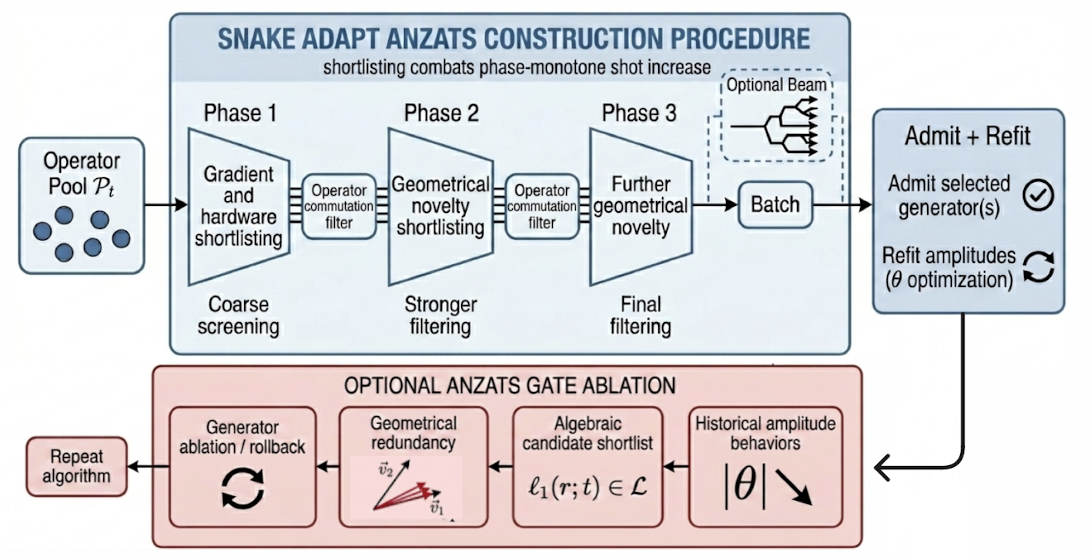
\includegraphics[width=\columnwidth]{figures/static_adapt_selector_flow_attached.png}
\captionof{figure}{SNAKE static ADAPT generator-selection flow. The broad generator pool is reduced through staged gradient--cost scoring, commutation filtering, physical operator-type shortlisting, final batch-compatible candidate-operator selection, beam branching for degenerate batches, and post-admission generator-ablation.}
\label{fig:static_adapt_selector_flow}
\end{center}

\label{sec:static_method}

\subsection{Staged generator-position ranking}
%
At ADAPT iteration \(k\), \textsc{SNAKE} evaluates candidate operator insertions on the current ordered ansatz \(U_k(\boldsymbol\theta_k^\star)\). Let \(p\) denote an admissible insertion position, and let \(\mathcal P_k\) denote the set of all such positions at iteration \(k\), so that \(p\in\mathcal P_k\). Similarly, let \(A\in\mathcal G\) denote an available generator in the operator pool. \textsc{SNAKE} then evaluates each generator--position record, written as
\[
r=(A,p)\in\mathcal G\times\mathcal P_k .
\]
We define the candidate generator--position record set at the current iteration \(k\) as
\begin{equation}
\mathcal R_k
=
\{r=(A,p)\mid A\in\mathcal G,\;p\in\Pcal_k\}
\subseteq\mathcal G\times\Pcal_k .
\label{record_set}
\end{equation}

At a given iteration \(k\), the \textsc{SNAKE} algorithm follows a four-phase staged restriction on the record set in Eq.~\eqref{record_set}. Because each progressive phase incorporates more expensive geometric and curvature information, each phase restricts the available record set that the next phase can rank. This shortlists candidates in proportion to our confidence that they are low-quality candidates, and thereby helps control subsequent measurement overhead.

Among this phase-restricted candidate record set, we further partition the set according to the operator's physical response channel, such as UCCSD-type operators versus phonon-dressed generators. This enables more aggressive shortlisting of the global pool by allowing different response-type generators to compete under different restrictive margins.

We then give Eq.~\eqref{record_set} explicit phase dependence. At a given ADAPT outer-loop iteration \(k\), index each phase by \(t\in\{0,1,2,3\}\), and initialize the recursion as \(\mathcal R^{(-1)}:=\mathcal R=\mathcal R_k\). We suppress the outer-iteration subscript \(k\) in the following phase-restriction definitions.

We then order each \(r\in\mathcal R^{(t-1)}\) based on a scoring function of the form
\begin{equation}
S^{(t)}(r)
=
\frac{\Delta E_t(r)\mathcal N_t(r)}{K_t(r)}\,,
\label{eq:master_phase_score}
\end{equation}
where \(\Delta E_t(r)\) is the phase-\(t\) state-gradient gain,
\(0\leq\mathcal N_t(r)\leq 1\) is the geometric novelty factor, which
down-weights candidates whose tangent directions are redundant with directions
already available in the ansatz, and \(K_t(r)\geq 1\) is the hardware-cost
penalty. Equation~\eqref{eq:master_phase_score} generalizes append-only
ADAPT's gradient ranking from a single generator score to a record-level
ranking that combines estimated energy gain, novelty, and cost normalization.
Without lane partitioning, the phase-\(t\) score would admit a phase-dependent
fixed number of the highest-scoring candidates to the next phase, until one or
more candidates are inserted in the batching process.

To prevent a numerically dominant cluster of physically similar records from
dominating the set advanced to the next phase, we partition the inherited record
set by physical response channel. The resulting lane-wise restriction preserves
representation of distinct response mechanisms whenever their best candidates
remain competitive, even if several nearly redundant records from another
channel score slightly higher under a pooled phase-wise ranking. We now define
the lane partition of \(\mathcal R\) through a partition of \(\mathcal G\). Let
\(\lambda:\mathcal G\to\mathcal L\) be a lane map for generators. The value
\(\lambda(A)=\ell\) is the physical operator-type label assigned to generator
\(A\). Let
\(\mathcal L^{(t-1)}\subseteq\mathcal L\) denote the lane labels represented in
the previously retained record set. For a lane label \(\ell\), define the
inherited lane records by
\begin{equation*}
\mathcal R_{\ell}^{(t-1)}
=
\{r=(A,p)\in\mathcal R^{(t-1)}
\mid \lambda(A)=\ell\}.
% source label: eq:lane_phase_records
\end{equation*}
The inherited lane records partition the previous phase record set
\(\mathcal R^{(t-1)}\).
For each lane label, the representative record is the within-lane maximizer
\[
r_{\ell}^{\star}\in
\operatorname*{arg\,max}_{r\in\mathcal R_{\ell}^{(t-1)}}S^{(t)}(r).
\]
This is the highest-scoring inherited record carrying label \(\ell\). The
corresponding global representative is \(r_{\mathcal L}^{\star}\in
\operatorname*{arg\,max}_{r\in\mathcal R^{(t-1)}}S^{(t)}(r)\),
the highest-scoring inherited record over the full lane-partitioned phase set.
A lane label \(\ell\) remains live at phase \(t\) when its best inherited
record is competitive with the best inherited record over the full
lane-partitioned phase set:
\begin{equation}
\ell\in\mathcal L^{(t)}
\quad\Longleftrightarrow\quad
S^{(t)}(r_{\ell}^{\star})
\ge
\tau_t
S^{(t)}(r_{\mathcal L}^{\star}).
\label{eq:phase_restriction_map}
\end{equation}
Here \(\tau_t\) is the phase-\(t\) relative lane-retention threshold. The
number of live lanes that receive protected representatives is
\begin{equation}
\min\left\{
N_t,\,
\left\lceil \rho_t|\mathcal L^{(t)}|\right\rceil
\right\},
\qquad
|\mathcal R^{(t)}|\le N_t ,
\label{eq:phase_lane_budget}
\end{equation}
where \(N_t\) is the phase-\(t\) global retained-record cap and
\(0<\rho_t\le 1\) is the live-lane protection fraction. Subject to this cap,
live lanes are ordered by their best phase-\(t\) score
\(S^{(t)}(r_{\ell}^{\star})\), and the top protected-lane count receives one
record per lane. Remaining capacity is filled by the next highest-scoring records
drawn from the live lanes.
The resulting ansatz update is written as:
%
\begin{equation*}
U_{k+1}(\boldsymbol\theta_{k+1})
=
U_k(\boldsymbol\theta_k)
\oplus
\bigcup_{r\in\mathcal B} r
\ominus
\bigcup_{d\in\mathcal D} d .
% source label: eq:snake_ansatz_update
\end{equation*}
%
Here $\mathcal B$ is the batch-admissible set of retained Phase-III records, and $\mathcal D$ is the ablation-admissible set of existing ansatz entries. The symbol \(\oplus\) denotes admission of selected generator records into the ordered ansatz, and \(\ominus\) denotes removal of ablation-admissible existing records. Before discussing in detail the different stages of candidate selection, we will explain how the hardware cost penalty and candidate gradients are computed in the next two sections.

\subsubsection{Hardware cost penalty}
%
\noindent
The hardware-cost penalty \(K_t(r)\) estimates the additional circuit and measurement burden introduced by selecting a new candidate record \(r\). This penalty is used to avoid selecting candidates that slightly improve the energy at the cost of a substantially larger circuit depth, two-qubit gate count, parameter space dimension, or measurement cost. We include five cost components in its definition: two-qubit gate count, layout-aware two-qubit depth, one-qubit basis-change work, additional variational parameters, and grouped-measurement shot demand.\\
\noindent
For a system of \(Q\) qubits, fix a candidate record \(r=(A,p)\). The associated compiled generator is expressed as a Pauli polynomial,

\begin{equation}
A=\sum_{\mu}c_{\mu}P_{\mu}, \qquad P_{\mu}\in\{I,X,Y,Z\}^{\otimes Q}\,.
\label{eq:pauli_expansion}
\end{equation}
%
For each nonzero Pauli word, we define its qubit support as
%
\begin{equation}
\begin{aligned}
S_{\mu}
&:=\operatorname{supp}(P_{\mu}) \\
&=\{q\in\{1,\ldots,Q\}:(P_{\mu})_q\ne I\}.
\end{aligned}
\label{eq:pauli_word_support}
\end{equation}
%
The cost estimates below are computed from these Pauli-word supports. Larger supports require longer parity-computation circuits, while supports spread across the hardware graph require larger entangling depth or routing overhead. For a Pauli exponential compiled by a CNOT ladder, a multi-qubit Pauli rotation is implemented by reducing it to a single-qubit rotation with additional entangling gates. A Pauli word acting on \(s=|S_{\mu}|\) qubits requires \(s-1\) \textsc{CNOT}s before the \(R_z\) rotation and \(s-1\) \textsc{CNOT}s after it to restore the original qubit register. The two-qubit gate count is estimated by
%
\begin{equation*}
\widehat C_{\twq}(r)=\sum_{\mu}2\,\max[|S_{\mu}|-1, 0],
% source label: eq:pauli_2count_proxy
\end{equation*}
whereas the layout-aware two-qubit depth is given by
\begin{equation*}
\widehat C_d(r)=\sum_{\mu}2\,\operatorname{span}_{G}
\bigl(S_{\mu}\bigr)\,.
% source label: eq:pauli_2depth_proxy
\end{equation*}
Here \(G\) is the hardware connectivity graph, and $\operatorname{span}_{G}(S_{\mu})$ is the number of edges in the shortest connected subgraph containing the support \(S_{\mu}\). The quantity is set to zero when $|S_{\mu}|\le1$. This term penalizes Pauli words whose active qubits are far apart in the connected graph.\\
\noindent
The same Pauli-rotation circuit also uses one-qubit basis-change gates. Let
\[
S_{\mu}^{XY} = \{q\in S_{\mu}:(P_{\mu})_q = X\text{ or }Y\}
\]
On each qubit in \(S_{\mu}^{XY}\), we rotate into the \(Z\) basis before the Pauli rotation and rotate it back afterward. Let \(c_q(g)\) denote the contribution of a one-qubit gate \(g\) on qubit \(q\) to this basis-change cost proxy. If the required basis rotation is $\beta_{\mu q}$, its forward and back cost is
\[
c_q^{\pm}(\beta_{\mu q})=c_q(\beta_{\mu q})+c_q(\beta^{-1}_{\mu q})\,.
\]
The one-qubit cost of this Pauli word is then given by
%
\begin{equation*}
\widehat{C}_{1q}^{(\mu)}(r) = \sum_{q\in S_{\mu}^{XY}}c_q^\pm(\beta_{\mu q}) + c_{\bar{q}_{\mu}}(R_z)\,.
\end{equation*}
Here \(\bar{q}_{\mu}\) is the qubit where the central rotation \(R_z\) is applied. The total one-qubit cost then becomes \(\widehat{C}_{1q}(r)=\sum_\mu\widehat{C}_{1q}^{(\mu)}(r)\). The parameter cost is the number of new independent parameters added by candidate \(r\):
\begin{equation*}
\widehat C_\theta(r)
=
|\boldsymbol\vartheta_r|.
% source label: eq:parameter_cost_proxy
\end{equation*}
%
Here \(\boldsymbol\vartheta_r\) is the parameter block introduced by record \(r\). For single generator insertion, this is one; however, batched or tied insertions may add a different number of independent parameters. For \(r=(A,p)\), insertion at position \(p\) conjugates the candidate generator by the part of the current ordered ansatz to the left of \(p\); equivalently, \(\widetilde A_r:=U_{>p}AU_{>p}^{\dagger}\), where \(U_{>p}\) denotes those left-positioned generators. Let \(H\) denote the encoded problem Hamiltonian. The measurement cost is computed from the candidate-gradient observable \cite{Verteletskyi2020CliqueCover,Yen2020CompatibleMeasurements}
\[
O_r:=i[\widetilde A_r,H]\,,
\]
after qubit mapping \(O_r\) is rewritten as a sum of Pauli words 
%
\[
O_r=\sum_{\nu=1}^{N_r}c_{r\nu}P_{r\nu}\,.
\]
%
Here \(N_r\) is the number of Pauli words in the mapped candidate-gradient operator, \(c_{r\nu}\) are Pauli coefficients, and \(P_{r\nu}\) are Pauli words.
The Pauli words are then grouped into qubit-wise commuting blocks, denoted by \(\Pi_r\), so that all Pauli words in the same block can be measured using a single basis. The goal is to estimate the additional number of shots required by candidate \(r\). Let \(\mathcal M\) be the set of measurement bases that have already been used in previous scoring steps. A block \(C\in\Pi_r\) has zero additional basis cost if it can be measured in one of these previously measured bases. We then denote \(C_r\subseteq\Pi_r\) as the set of blocks requiring no new measurement basis. As a consequence, only the blocks in \(\Pi_r\setminus C_r\) require a new measurement basis.
%with \(m_q\) the measured Pauli axis on qubit \(q\). The cached-basis blocks are
%\begin{equation}
%\begin{aligned}
%\mathcal C_r
%=
%\{C\in\Pi_r:\;&
%\exists m\in\mathcal M\;
%\forall \nu\in C\;
%\forall q,\\
%&
%(P_{r\nu})_q=I
%\ \lor\
%(P_{r\nu})_q=m_q
%\}.
%\end{aligned}
%\label{eq:cached_measurement_blocks}
%\end{equation}
For each new block \(C\), we assign the coefficient weight
\[
w_C = \sqrt{\sum_{\nu\in C}|c_{r\nu}|^2}\,.
\]
The shot-cost proxy is then given by
\begin{equation*}
\widehat C_{\rm shot}(r)=
\frac{1}{\sigma_\star^2}
\left[
\sum_{C\in\Pi_r\setminus C_r}
w_C
\right]^2\,.
% source label: eq:shot_cost_proxy
\end{equation*}
%
Here $\sigma_\star$ is the target standard error for the candidate-gradient estimate \cite{Ikhtiarudin2025ShotEfficient}. This proxy gives a lower cost to candidates whose gradient reuses existing measurement bases and a higher cost to candidates that require new measurement blocks with large Pauli coefficients.\\
For cost component \(x\), let \(m_x(t)\) and \(s_x(t)>0\) be the phase-\(t\) median and robust scale of \(\widehat C_x\) over the records being scored. For a given cost term component $\widehat C_x$, the normalized excess cost is given by
%
\begin{equation}
\bar C_x(r;t):=
\operatorname{asinh}
\left(
\frac{\text{max}[\widehat C_x(r)-m_x(t), 0]}{s_x(t)}
\right),
\label{eq:cost_robust_excess}
\end{equation}
%
Thus, a candidate is penalized only when its cost exceeds the phase-\(t\) median. The inverse-hyperbolic-sine transform keeps the penalty approximately linear for moderate excess costs while compressing very large outliers \cite{IglewiczHoaglin1993,Burbidge1988IHS}.
The phase-\(t\) hardware-cost penalty then is one plus the weighted sum of these robust-normalized excess costs,
\begin{equation}
\begin{aligned}
K_t(r)
={}&
1+\lambda_{\twq}\bar C_{\twq}(r;t)
+\lambda_d \bar C_d(r;t)\\
&+\lambda_{1q}\bar C_{1q}(r;t)
 +\lambda_\theta \bar C_\theta(r;t)\\
&+\lambda_{\rm shot}\bar C_{\rm shot}(r;t)\,.
\end{aligned}
\label{eq:hardware_cost_sum}
\end{equation}
%
Each barred quantity in Eq.~\eqref{eq:cost_robust_excess} is the robust excess version of the corresponding raw proxy: two-qubit gate count, layout-aware depth, one-qubit basis-change cost, parameter cost, and shot cost. The weights \(\lambda_{\twq}\), \(\lambda_d\), \(\lambda_{1q}\), \(\lambda_\theta\), and \(\lambda_{\rm shot}\) set the relative importance of these resources.

\subsubsection{Candidate gradient}
%
\noindent
For a candidate record \(r=(A,p)\) at ADAPT iteration \(k\), the magnitude of the candidate gradient is
\begin{equation}
\begin{aligned}
g:=g(r)
&=
\left|
\left.
\partial_\alpha
\langle\psi_k|
e^{i\alpha\widetilde A_r}
H
e^{-i\alpha\widetilde A_r}
|\psi_k\rangle
\right|_{\alpha=0}
\right|\\
&=
\left|\langle\psi_k|O_r|\psi_k\rangle\right| .
\end{aligned}
\label{eq:record_gradient}
\end{equation}
%
We can now move on to discuss the different phases of the ansatz construction procedure.

\subsubsection{Phase 0}
%
\noindent
Phase 0 is the inexpensive first-pass screening stage. It is obtained from Eq.~\eqref{eq:phase0_score} by using only the standard first-order ADAPT gradient and the phase-0 hardware-cost penalty. For the fixed candidate record \(r=(A,p)\), the Phase-0 score is
%
\begin{equation}
S_{0}(r)=\frac{\alpha_0 g}{K_0(r)}\,.
\label{eq:phase0_score}
\end{equation}
%
Here \(\alpha_0>0\) is a fixed pre-screening scale factor, \(g\) is the gradient magnitude from Eq.~\eqref{eq:record_gradient}, and \(K_0(r)\) is the phase-0 cost penalty. This stage is intentionally non-aggressive: its purpose is not to make the final generator-selection decision, but to remove candidates with both small gradient signals and large estimated costs before more expensive evaluations are performed. Records are passed to Phase I when their lane-wise score exceeds the threshold \(\tau_{0,\ell}\). To avoid discarding all useful candidates in a low-signal iteration, a fallback rule also retains the top-ranked records in each lane.

\subsubsection{Physical operator-type shortlisting}
\label{subsec:hh_physical_operator_lanes}
%
Between scoring phases, \textsc{SNAKE} partitions Hubbard--Holstein
generator--position records into six physical lanes. The lane label is determined only by the
physical role of the candidate generator, not by its Pauli support or its
commutation relation with the current ansatz. The purpose is to preserve
exposure for qualitatively different response mechanisms before the expensive
geometric and curvature phases are evaluated.

\paragraph*{Electronic UCCSD lane.}
This lane contains bare electronic single- and double-excitation generators,
tensored with the phonon identity:
\begin{align*}
G_{i\to a,\sigma}
&=
\ii(c_{a\sigma}^{\dagger}c_{i\sigma}
-c_{i\sigma}^{\dagger}c_{a\sigma}),\\
G_{ij\to ab,\sigma\sigma'}
&=
\ii(c_{a\sigma}^{\dagger}c_{b\sigma'}^{\dagger}
c_{j\sigma'}c_{i\sigma}
-{\rm h.c.}) .
\end{align*}
Here \(i,j\) label occupied spin orbitals, \(a,b\) label virtual spin orbitals,
\(\sigma,\sigma'\in\{\uparrow,\downarrow\}\), and \(c^\dagger,c\) are
fermionic creation and annihilation operators. This lane targets electronic
correlation without explicit phonon dressing.

\paragraph*{Electronic hopping/current lane.}
This lane contains purely electronic Hubbard transport, density-assisted
transport, pair-hop/current, and exchange/current channels, all acting with the
phonon identity. The spin-summed hopping and current generators are
\begin{align*}
T_{ij}
&=
\sum_{\sigma}
(c_{i\sigma}^{\dagger}c_{j\sigma}
+c_{j\sigma}^{\dagger}c_{i\sigma}),\\
J_{ij}
&=
\ii\sum_{\sigma}
(c_{i\sigma}^{\dagger}c_{j\sigma}
-c_{j\sigma}^{\dagger}c_{i\sigma}) .
\end{align*}
Density-assisted channels multiply \(T_{ij}\) or \(J_{ij}\) by local fermion
number operators. Pair-hop/current channels move an onsite spin pair between
sites. Exchange/current channels exchange spin-resolved occupations across a
bond. This lane targets lattice electronic motion beyond bare UCCSD excitation
structure.

\paragraph*{Phonon-cloud lane.}
This lane contains pure phonon displacement, momentum, and occupation channels.
Here \(b_i^\dagger,b_i\) are phonon creation and annihilation
operators on site or mode \(i\), and
\[
X_i=b_i+b_i^\dagger,
\qquad
P_i=\ii(b_i^\dagger-b_i),
\qquad
n_{b,i}=b_i^\dagger b_i .
\]
The Hubbard--Holstein lane includes the local phonon generators \(X_i\),
\(P_i\), and \(n_{b,i}\), together with nonlocal charge--phonon cloud terms
listed below in the dressed electron--phonon lane. This lane targets the
displacement and occupation response of the phonon cloud before explicit
electronic conditioning is applied.

\paragraph*{Phonon-relaxation lane.}
This lane contains pure phonon squeeze, width, quadratic, and nonlinear
channels:
\begin{align*}
S_i&=\ii[(b_i^\dagger)^2-b_i^2],\\
&X_i^2,\quad P_i^2,\quad n_{b,i}^2,\quad
X_iP_i+P_iX_i .
\end{align*}
This lane targets changes in local phonon width, occupation curvature, and
cutoff-sensitive nonlinear response.

\paragraph*{Dressed electron--phonon lane.}
This lane contains generators that explicitly couple electronic charge or bond
motion to phonon response. With
\[
D_i=n_i-\bar n I,
\qquad
Q_i=n_{i\uparrow}n_{i\downarrow},
\]
it includes local polaronic channels \(D_iP_i\) and \(D_iS_i\), nonlocal
charge--phonon channels \(D_iP_j\) and \(D_iX_j\), doublon-conditioned channels
\(Q_iP_j\) and \(Q_iX_j\), and bond-dressing channels
\begin{align*}
&T_{ij}(P_i-P_j),
\qquad
J_{ij}(P_i-P_j),\\
&T_{ij}(P_i+P_j),
\qquad
T_{ij}(P_i-P_j)^2,\\
&J_{ij}(P_i-P_j)^3 .
\end{align*}
It also includes UCCSD electronic generators multiplied by phonon-dressing
operators, including product and sequential electronic/phonon motif generators.
This lane targets polaron formation, density-conditioned lattice response,
doublon-conditioned lattice response, and bond-conditioned electron--phonon
dressing.

\paragraph*{Hamiltonian-block lane.}
This lane contains grouped physical blocks of the Hubbard--Holstein Hamiltonian
in Eq.~\eqref{eq:hubbard_holstein_static}: electronic hopping, onsite
interaction, phonon energy, and electron--phonon coupling blocks, together with
the full Hamiltonian-block rotation when included. It also includes
Hamiltonian-term generators and their quadrature partners. This lane preserves
coarse Hamiltonian structure as candidate ansatz motion.

Within each lane, records are ordered by the current phase score and shortlisted
using the live-lane restriction and retained-record cap in
Eqs.~\eqref{eq:phase_restriction_map}--\eqref{eq:phase_lane_budget}. The score
itself is unchanged. The physical-lane partition only controls which records
compete against one another during shortlisting, so electronic correlation,
electronic transport, phonon cloud motion, phonon relaxation, dressed
electron--phonon response, and Hamiltonian-block motion compete within
physically matched lanes before the protected-lane and retained-record caps are
applied.

\paragraph*{Inverse Notation.}
%All inverse solves below use the damped, supported version of the displayed block. For Gram blocks, \(G^+\) denotes the Moore--Penrose inverse on the retained tangent support. We suppress explicit inverse-regularization terms in the displayed scoring equations.
Some of the scores below require inverses of Gram, metric, or Hessian matrices. These matrices may be singular when the local tangent space contains redundant directions or when a candidate generator has very little effect on the current state. Therefore, every inverse below should be understood as a regularized pseudoinverse. We use \(G^+\) for the Moore-Penrose pseudoinverse after removing numerically null directions. The same convention is used for metric and Hessian matrices. To keep the equations readable, we avoid writing the damping and projection steps explicitly.

\subsubsection{Phase I}
%
\noindent
Phase I replaces the purely gradient-based prescreening with a geometry-normalized local energy gain estimate. For a fixed candidate record \(r\), the ADAPT gradient is evaluated together with the Fubini--Study norm of the candidate tangent \cite{Nocedal2006TrustRegion}; we suppress the \(r\)-dependence of \(g\), \(F\), \(\tau\), and \(\alpha^\star\) in this local model. In this way, Phase I estimates how much the candidate record \(r\) can lower the energy before it displaces the current variational state beyond a certain value \(\rho\). The candidate is assigned a trial amplitude \(\alpha\); for each value of \(\alpha\) \textsc{SNAKE} estimates the energy gain \(\Delta E_{1}(r)\) using a one-dimensional quadratic descriptor. The allowed values of \(\alpha\) are then restricted by the condition that the Fubini--Study displacement does not exceed \(\rho\),
%
\begin{equation}
\begin{split}
\Delta E_{1}(r)={}&\max_{\alpha^2F\le \rho^2} \left[g\alpha-\frac{1}{2}F\alpha^2\right],
\end{split}
\label{eq:phase1_gain}
\end{equation}
%
where \(g\) is given by Eq.~\eqref{eq:record_gradient}. The factor \(F\) measures how strongly candidate record \(r\) moves the current variational state. To define it, let \(\Pi=I-\ket{\psi}\bra{\psi}\) be the projector onto the subspace orthogonal to the current state, and let \(\ket{\psi(\alpha;r)}=e^{\alpha\widetilde A_r}\ket{\psi}\). The candidate tangent is \(\tau=\left.\partial_\alpha\ket{\psi(\alpha;r)}\right|_{\alpha=0}\). The diagonal Fubini--Study scale is then given by
%
\begin{equation*}
F=\|\Pi\tau\|^2.
% source label: eq:phase1_tangent_scale
\end{equation*}
%
The parameter maximizer in Eq.~\eqref{eq:phase1_gain} is then defined by taking the following minimum
\begin{equation}
\alpha^\star
=
\min\!\left(
\dfrac{g}{F},
\dfrac{\rho}{\sqrt{F}}
\right)\,.
\label{eq:phase1_alpha_star}
\end{equation}
The value is then used to obtain the Phase-I gain \(\Delta E_1(r)\), which is subsequently used in the Phase-I score \(S_1(r)\). If the candidate is finally admitted to the ansatz, \(\alpha^\star\) initializes the newly inserted generator coordinate, which is then optimized together with the active ansatz parameters under the chosen inner optimization procedure in Eq.~\eqref{eq:theta_opt}.

\subsubsection{Phase II}

The top-ranked records from Phase I then pass into Phase II, which refines the local quadratic trust-region energy model with second-order curvature, and weights candidates using a novelty bonus based on whether the local ansatz tangent span can express the candidate's induced tangent. 

The trust-region constrained second-order energy estimate is given by
\begin{equation*}
\Delta E_{2}(r)
=\max_{|\alpha|\sqrt{F}\le\rho}
\Bigl[g\alpha -\frac{h\alpha^2}{2}\Bigr],
% source label: eq:phase2_gain
\end{equation*}
where the directional energy curvature is
\begin{align*}
h&=
2\Re\!\left[
(\partial_{\alpha}\langle \psi|)H|\partial_{\alpha}\psi\rangle
+\langle\psi|H|\partial^2_{\alpha}\psi\rangle
\right],
% source label: eq:phase2_hessian
\end{align*}
  
and $\partial^2_{\alpha}\ket{\psi} =-(U_{>p}AU_{>p}^{\dagger})^2\ket{\psi}.$ Here \(>p\) denotes the ansatz generators to the left of position index \(p\), where the rightmost generator is index \(1\). The reported score retains only positive directional curvature. The trial amplitude uses Eq.~\eqref{eq:phase1_alpha_star} with the substitution \(g/F \to g/h\), while \(\rho/\sqrt{F}\) remains unchanged. This amplitude warm-starts the newly inserted generator coordinate for admitted records.

For \(r\), let \(W_r\) be the capped reduced-geometry refit-coordinate window, with \(i,j\in W_r\). The Fubini--Study Gram matrix on this coordinate block and the candidate tangent-covariance vector are given by
\begin{equation*}
(G)_{ij}=\Re\langle\tau_i,\tau_j\rangle,
\qquad
(q)_i=\Re\langle\tau_i,\tau\rangle.
\end{equation*}
The Phase-II novelty term is the normalized least-squares component of the candidate tangent lying outside the \(W_r\)-tangent span:
\begin{equation}
\begin{aligned}
\mathcal N_2(r)
&:=
\frac{1}{F}
\min_{\gamma}
\left\|
\Pi\left(\tau-\sum_{i\in W_r}\gamma_i\tau_i\right)
\right\|^2 \\
&=
1-
\frac{q^{\top}G^+q}{F}.
\end{aligned}
\label{eq:phase2_novelty}
\end{equation}
Thus $\mathcal N_2(r)$ is small when the \(W_r\)-tangent span already contains $\tau$, and large when the candidate contributes an independent state-space direction.

\subsubsection{Generator Pauli-Splitting}
For generator records retained by the Phase-II shortlist, \textsc{SNAKE}
employs a qubit-ADAPT-VQE-style Pauli splitting to enumerate
hardware-efficient ansatz generators \cite{Tang2021}. For the record
\(r=(A,p)\), with Pauli expansion given by Eq.~\eqref{eq:pauli_expansion}, let
\(J\) define a subset of the Pauli-word support of \(A\), and let
\(r_J=(A_J,p)\) be the corresponding child record. The child generator is
\begin{equation*}
A_J=\sum_{\mu\in J}c_{\mu}P_{\mu}.
% source label: eq:pauli_child_generator
\end{equation*}
Here \(P_{\mu}\) is the \(\mu\)th Pauli word in the expansion of the fixed
generator \(A\), and \(c_{\mu}\) is its scalar Pauli coefficient.
For this generator, the generator-level support is
\begin{equation}
\operatorname{supp}(A)
:=
\bigcup_{\mu:c_{\mu}\ne0}
\operatorname{supp}(P_{\mu}).
\label{eq:macro_generator_support}
\end{equation}
Equations~\eqref{eq:pauli_word_support} and~\eqref{eq:macro_generator_support}
show that
\(\operatorname{supp}(A_J)\subseteq\operatorname{supp}(A)\). We then apply
the fermionic sector-preserving test \(\Gamma(A_J)\) defined below to the
child generator:
\begin{equation}
\Gamma(A_J)
=
\prod_{s\in\{\uparrow,\downarrow,\mathrm{total}\}}
\mathbf 1
\left\{
\left\|
\left[
A_J,\mathbf N_s^{(f)}\otimes \mathbb I^{(b)}
\right]
\right\|_1
\le \epsilon
\right\}.
\label{eq:symmetry_guard}
\end{equation}
Here \(\mathbf 1\{\cdot\}\) is the indicator function. The operator \(\mathbf N_s^{(f)}\) is the fermionic number operator for sector \(s\), where \(s\) denotes spin up, spin
down, or total particle number; we tensor \(\mathbf N_s^{(f)}\) with the boson
register identity operator. The parameter \(\epsilon\) is a leakage-tolerance
parameter. The Pauli-coefficient \(L^1\) norm is defined by summing the absolute
coefficients of the Pauli polynomial after taking the commutator in
Eq.~\eqref{eq:symmetry_guard}. Explicitly, suppose the commutator gives
\([A_J,\mathbf N_s^{(f)}\otimes \mathbb I^{(b)}]
=\sum_\nu b_\nu^{(s,J)}P_\nu\). Then the \(L^1\) norm is
\[
\left\|
\left[
A_J,\mathbf N_s^{(f)}\otimes \mathbb I^{(b)}
\right]
\right\|_1
=
\sum_\nu |b_\nu^{(s,J)}|.
\]

These symmetry-retained operator-children then act as the new shortlisted
operator set for subsequent Phase-III scoring and batching. We omit explicit
\(J\)-dependence below for visual simplicity, and assume all records
\(r=(A,p)\) may be Pauli-word combinations with subset generator support of
the generator \(A\).
\subsubsection{Phase III}

Phase III performs Schur-refit reranking over candidate-specific refit-coordinate windows.

The energy gain model is
\begin{equation}
\Delta E_{3}(r)=
\max_{|\alpha|\sqrt{F^\star}\le\rho}
\left[g\alpha-\frac{h^\star \alpha^2}{2}\right].
\label{eq:phase3_gain}
\end{equation}
Here $F^\star$ and $h^\star$ are defined in Eqs.~\eqref{eq:phase3_star_geometry} and~\eqref{eq:phase3_schur_response} and represent the predicted Fubini--Study metric and the energy-curvature after admitting $r$ and allowing the existing ansatz $U_k(\theta_k)$ to reoptimize. The selected $\alpha^\star$ is given by Eq.~\eqref{eq:phase1_alpha_star} under the substitution $g/F \to g/h^\star$ and $\rho / \sqrt{F} \to \rho / \sqrt{F^\star}$.

Let $\delta\theta$ be the response parameter vector with indices in \(W_r\subseteq\{1,\ldots,|\boldsymbol{\theta}_k|\}\). Phase III assumes a local quadratic model in which the candidate operator's energy gain is coupled to this refit-window response after admitting $r$.
Let \(c\) denote the candidate-window coupling vector and let \(\mathbf H\) denote the Hessian block over the refit-coordinate window \(W_r\), with entries defined below. Explicitly, 
\begin{equation}
\begin{split}
E(\alpha,\delta\theta)\approx{}&E_0-g\alpha+\frac{h\alpha^2}{2} \\
&+\alpha c^{\top}\delta\theta
+\frac{\delta\theta^{\top}\mathbf{H}\delta\theta}{2},
\end{split}
\label{eq:local_quadratic}
\end{equation}
where \(E_0=E(U_k(\boldsymbol\theta_k^\star))\) is the current optimized ansatz energy. Here $c$ couples the candidate to the \(W_r\)-coordinate response and $\mathbf{H}$ is the corresponding Hessian block; entries are given by
\begin{equation}
\begin{aligned}
c_j&:=
\left.
\frac{\partial^2E(\alpha,\delta\theta)}
{\partial\alpha\,\partial(\delta\theta_j)}
\right|_0,\\
\mathbf{H}_{jk}&:=
\left.
\frac{\partial^2E(\alpha,\delta\theta)}
{\partial(\delta\theta_j)\,\partial(\delta\theta_k)}
\right|_0,
\qquad j,k\in W_r .
\end{aligned}
\label{eq:phase3_window_derivatives}
\end{equation}
Let \(\mathbf R\) denote the symmetrized \(W_r\)-supported Hessian block used in the refit solve:
\begin{equation}
\mathbf R=\frac12(\mathbf H+\mathbf H^{\top}).
\label{eq:phase3_regularized_hessian}
\end{equation}

Eliminating the \(W_r\) coordinates by optimizing Eq.~\eqref{eq:local_quadratic} over $\delta\theta$ gives the optimal local refit response induced by the candidate, and substituting it back into Eq.~\eqref{eq:local_quadratic} yields the Schur-relaxed curvature $h^\star$. Explicitly,
\begin{equation}
\delta\theta^\star=-\alpha\mathbf R^{-1}c,
\qquad
h^\star=h-c^{\top}\mathbf R^{-1}c .
\label{eq:phase3_schur_response}
\end{equation}
Eqs.~\eqref{eq:phase3_window_derivatives}--\eqref{eq:phase3_regularized_hessian} give the ideal Schur model; the inverse and damping convention is the one stated above
and also applies to the batch Schur blocks below. Evaluating $\delta\theta^\star$ at the selected trial amplitude $\alpha^\star$ gives the inherited-coordinate warm-start seed for the inner re-optimization on the enlarged ansatz. Dividing $\delta\theta^\star$ by $\alpha$ gives the inherited-coordinate compensation per unit candidate amplitude. This defines the Schur-reduced residual tangent, Schur-reduced Fubini--Study norm, and Schur-reduced candidate--ansatz overlap:
\begin{equation}
\begin{aligned}
\tau^\star
&=\tau+\sum_{i\in W_r}\left(\frac{\delta\theta^\star}{\alpha}\right)_i\tau_i,\\
F^\star
&=F+2q^{\top}\frac{\delta\theta^\star}{\alpha}
+\frac{(\delta\theta^\star)^{\top}}{\alpha}G\frac{\delta\theta^\star}{\alpha},\\
q^\star
&=q+G\frac{\delta\theta^\star}{\alpha}.
\end{aligned}
\label{eq:phase3_star_geometry}
\end{equation}
This completes Eq.~\eqref{eq:phase3_gain}, and enables a least-squares treatment, analogous to Eq.~\eqref{eq:phase2_novelty}, to define a Phase-III novelty factor:
\begin{equation}
\begin{aligned}
\mathcal N_3(r)
&:=
\frac{1}{F^\star}
\min_{\gamma}
\left\|
\Pi\left(\tau^\star-\sum_{i\in W_r}\gamma_i\tau_i\right)
\right\|^2 \\
&=
1-\frac{(q^\star)^{\top}G^+q^\star}
{F^\star}.
\end{aligned}
\label{eq:phase3_novelty}
\end{equation}

\subsubsection{Batching}
Let \(B=\{r_1,\ldots,r_s\}\subseteq\mathcal R_k^{(3)}\) denote a set of eligible batch candidates retained after Phase III by Eq.~\eqref{eq:phase_restriction_map}. An optional conservative batch shortlist restricts \(B\) to records with disjoint qubit support and mutual commutation.

For batch-local indices \(a,b=1,\ldots,s\) and capped batch refit-coordinate window \(W_B\), let $H_{BB}=[\partial_{\alpha_a}\partial_{\alpha_b}E]_{a,b=1}^s$ be the Hessian block among candidate amplitudes, and let $H_{W_BB}=[\partial_{\theta_i}\partial_{\alpha_a}E]_{i\in W_B,\,a=1,\ldots,s}$ be the mixed window-candidate block. Then, with $H_{W_BW_B}=[\partial_{\theta_i}\partial_{\theta_j}E]_{i,j\in W_B}$ and $\mathbf R_B=\frac12(H_{W_BW_B}+H_{W_BW_B}^{\top})$, the Schur-refit batch curvature, residual tangents, and reduced Gram matrix are
\begin{equation*}
\begin{aligned}
H_B^\star
&=
H_{BB}
-
H_{BW_B}\mathbf R_B^{-1}H_{W_BB},\\
\tau_a^\star
&=\tau_a-\sum_{i\in W_B}(\mathbf R_B^{-1}H_{W_BB})_{ia}\tau_i,\\
(G_B^\star)_{ab}
&=\Re\langle \Pi\tau_a^\star,\Pi\tau_b^\star\rangle .
\end{aligned}
% source label: eq:batch_schur_curvature
\end{equation*}

For an induced gradient vector of $B$, define \(g_B=\big(g_{r_1},\ldots,g_{r_s}\big)^\top\). This enables an expected batch gain,
\begin{equation*}
\Delta E_3(B)
=
\max_{\alpha_B^\top G_B^\star\alpha_B\le \rho_B^2}
\left[
g_B^\top\alpha_B
-
\frac12\alpha_B^\top H_B^\star\alpha_B
\right],
% source label: eq:batch_expected_gain
\end{equation*}
Here \(\alpha_B=(\alpha_1,\ldots,\alpha_s)^\top\) is the batch-amplitude vector, \(\rho_B\) is the batch trust-region radius, and \(K_3(B)\) is the cost term from Eq.~\eqref{eq:hardware_cost_sum} evaluated over the batch. The admitted batch is therefore
\begin{equation}
B^\star\in\arg\max_{B\subseteq\mathcal R_k^{(3)}}\frac{\Delta E_3(B)}{K_3(B)}.
\label{eq:batch_argmax}
\end{equation}
Equation~\eqref{eq:batch_argmax} is the combinatorial search ideal, although a score-ordered greedy admission serves as a measurement-cheap practical approximation. 

\subsubsection{Beaming}
\textsc{SNAKE} borrows Lowerre-style beam search to branch candidate circuits in parallel \cite{Lowerre1976Beam}. Given a score-ordered top-$N$ candidate-batch list, a parent circuit can spawn $N$ child branches, with each child differing by the batched candidate admitted to that branch. The cost of this parallel beam universe is increased total hardware-graph and qubit support across candidate child circuits. Each child branch then undergoes the generator-ablation procedure described next. Under a fixed beam capacity, branch retention and termination follow the hardware-cost-weighted energy-dominance ordering among child branches.


\subsubsection{Generator ablation}
Generator ablation acts after a generator is admitted and the inner optimizer
refits the current ansatz. We propose an objective given by
Eq.~\eqref{eq:schur_metric_prune} which models the Schur response energy and
state-displacement response of the ansatz circuit under removal of a candidate
generator. Let \(\mathbf A_k=(A_1,\ldots,A_{n_k})\) be the ordered generator
sequence defining the current optimized ansatz \(U_k(\boldsymbol\theta_k^\star)\).
Each active generator \(A_j\) carries an admission step \(a_j\) and a cooldown
counter \(c_j(k)\). Equivalently, if \(\hat r_j\) is the most recent rejected
delete/refit trial for \(A_j\), a fixed cooldown requires
\(k-\hat r_j\ge\tilde c\); if no such rejection exists, the cooldown condition
is satisfied. The deletion-eligible coordinates are
\begin{equation*}
\mathcal E_k^\ominus
=
\left\{
j\in\{1,\ldots,n_k\}
:
k-a_j\ge \tilde p,\;
c_j(k)\le0
\right\}.
% source label: eq:eligibility_set
\end{equation*}
Here \(\tilde p\) and \(\tilde c\) are run-time constant protection thresholds.

Then, for \(j\in\mathcal E_k^\ominus\), we predict the Schur response energy
loss under the ablation of \(A_j\), together with the ability of the ansatz to
recover the pre-ablation state by minimizing the Fubini--Study metric
displacement. Define the surviving ansatz-generator index set as
\[
D:=\{1,\ldots,n_k\}\setminus\{j\},
\qquad
|D|=n_k-1 .
\]
Let \(u,v\in D\) denote surviving-coordinate indices. All quantities below are
evaluated at \(U_k(\boldsymbol\theta_k^\star)\):
\[
\tau_u
=
\left.
\partial_{\theta_u}\ket{\psi(U_k,\boldsymbol\theta)}
\right|_{\boldsymbol\theta=\boldsymbol\theta_k^\star},
\qquad
G_{uv}
=
\operatorname{Re}\langle \Pi_k^\star\tau_u,\Pi_k^\star\tau_v\rangle,
\]
where \(\Pi_k^\star\) is the projector onto the subspace orthogonal to the current optimized state.
\[
g_u
=
\left.
\partial_{\theta_u}E(U_k,\boldsymbol\theta)
\right|_{\boldsymbol\theta=\boldsymbol\theta_k^\star},
\qquad
H_{uv}
=
\left.
\partial_{\theta_u}\partial_{\theta_v}E(U_k,\boldsymbol\theta)
\right|_{\boldsymbol\theta=\boldsymbol\theta_k^\star}.
\]

We define the metric-regularized Schur ablation surrogate as
\begin{equation}
\begin{aligned}
\Lambda(A_j)
=
\min_{\delta\theta_D}
\Biggl[
&\Lambda_E(A_j,\delta\theta_D)
\\
&+
\frac{\eta}{2}
\left\|
\Pi_k^\star
\left(
-\theta_{k,j}^\star\tau_j
+
\sum_{u\in D}\delta\theta_u\tau_u
\right)
\right\|^2
\Biggr].
\end{aligned}
\label{eq:schur_metric_prune}
\end{equation}
The parameter \(\eta\ge0\) controls the Fubini--Study regularization of the
ablation Schur model.
The local energy term is the deletion specialization of the Phase-III
quadratic model in Eq.~\eqref{eq:local_quadratic}:
\begin{equation*}
\begin{aligned}
\Lambda_E(A_j,\delta\theta_D)
={}&
-g_j\theta_{k,j}^\star
+
\frac12(\theta_{k,j}^\star)^2H_{jj}
\\
&-
\theta_{k,j}^\star H_{Dj}^{\top}\delta\theta_D
+
\frac12\delta\theta_D^{\top}H_{DD}\delta\theta_D .
\end{aligned}
% source label: eq:lambda_schur_energy_loss
\end{equation*}
Define the metric-regularized quadratic block
\[
\mathcal Q:=H+\eta G .
\]
The optimal Schur response becomes
\begin{equation*}
\begin{aligned}
\delta\boldsymbol\theta_D^\star
&=
\theta_{k,j}^\star
\mathcal Q_{DD}^{+}\mathcal Q_{Dj}
\\
&=
\theta_{k,j}^\star
\left(H_{DD}+\eta G_{DD}\right)^+
\left(H_{Dj}+\eta G_{Dj}\right).
\end{aligned}
% source label: eq:ablation_schur_response
\end{equation*}
Substitution into Eq.~\eqref{eq:schur_metric_prune} gives
\begin{equation*}
\begin{aligned}
\Lambda(A_j)
={}&
-g_j\theta_{k,j}^\star
+
\frac12(\theta_{k,j}^\star)^2\mathcal Q_{jj}
\\
&-
\frac12(\theta_{k,j}^\star)^2
\mathcal Q_{Dj}^{\top}
\mathcal Q_{DD}^{+}
\mathcal Q_{Dj}.
\end{aligned}
% source label: eq:ablation_schur_loss
\end{equation*}

To prefer deletions that relieve larger compiled and measurement burden, let
\(K_j\) be the same normalized hardware/shot-cost denominator used in the SNAKE
candidate scores, evaluated over the current ansatz-entry population. Schur
pruning nominates generators whose predicted metric-regularized deletion loss
is small relative to the hardware and estimator burden they remove. The ratio
\(\Lambda(A_j)/K_j\) is clipped to the interval \([0,1]\) before nomination.
Generator ablation \(\mathbf A_k\ominus A_{j^\star}\) is determined by
\begin{equation*}
j^\star
\in
\operatorname*{arg\,min}_{j\in\mathcal E_k^\ominus}
\frac{\Lambda(A_j)}{K_j},
\qquad
\frac{\Lambda(A_{j^\star})}{K_{j^\star}}
\le
\epsilon .
% source label: eq:ablation_nomination
\end{equation*}
If the second condition fails, no ablation is nominated at this adaptive step.
After a candidate deletion, the ablation is accepted only if the realized energy
loss \(\Delta E(A_{j^\star})\) is no larger than the smaller of the absolute
ablation tolerance \(\epsilon\) and the fractional recent-gain tolerance
\(\rho\left(E(U_{k-1})-E(U_k)\right)\), where \(0\le\rho\le1\).

If this acceptance gate rejects the trial ablation, the post-refit
branch remains \(U_k(\boldsymbol\theta_k^\star)\). This allows the Gram block results to be
reused in Eqs.~\eqref{eq:phase2_novelty}, \eqref{eq:phase3_star_geometry}, and
\eqref{eq:phase3_novelty}; similarly, the Hessian block is reused in
Eqs.~\eqref{eq:phase3_window_derivatives}--\eqref{eq:phase3_schur_response}.
The Phase-III displacement coordinates are local
shifts, \(\theta=\theta^\star+\delta\theta\), so derivatives in
\(\delta\theta\) at \(\delta\theta=0\) reuse the same \(G\) and \(H\)
subblocks. Conversely, if the acceptance gate accepts the ablation, subsequent Phase-II/III
scoring recomputes \(G\) and \(H\) on the refit pruned circuit
\(U_k^{\ominus}((\boldsymbol\theta_k^\star)_{\setminus j^\star})
=
U_k(\boldsymbol\theta_k^\star)\ominus
\exp(\theta_{k,j^\star}^\star A_{j^\star})\), where \((\boldsymbol\theta_k^\star)_{\setminus j^\star}\) represents the optimized circuit parameterization after removing coordinate \(j^\star\).



\subsection{Stopping condition}
The outer adaptive loop repeats phases zero through three, followed by batch, beam, and generator-ablation, until one of three conditions holds: the maximum outer-loop iteration budget is reached, the maximum compiled circuit-cost budget is saturated, or a gradient plateau below a predefined threshold persists for a prescribed patience period.

%\end{comment} 


\section{Results}
\label{sec:results}
\label{sec:benchmarks}

We frame the advantage of SNAKE in terms of reducing energy error and circuit-resource metrics compared to append-only ADAPT-VQE and the recently released Geo-ADAPT-VQE on an equally physically parameterized two-site Hubbard--Holstein model. 

Supplementary appendices reserve result slots for dimer lattice models of Hubbard, Bose--Hubbard, and spin-boson/Rabi; we further include an instance of the three-site Hubbard--Holstein model. All fermion-containing models use half filling, and all lattice models use open boundary conditions. The Hubbard--Holstein generator pool is defined in Sec.~\ref{subsec:hh_physical_operator_lanes}, and the SPSA inner-optimization schedule is recorded in Appendix~\ref{app:spsa_settings}. The reported Hubbard--Holstein comparison displays SNAKE, Geo-ADAPT, and append-only ADAPT using the same inner-optimization method. Geo-ADAPT and append-only ADAPT use the generator pool before Pauli-child splitting; symmetry-retained singleton Pauli-child comparator runs are retained as supplemental sensitivity checks but omitted from the main reported rows.

We report energy error as the absolute difference between the ADAPT-resolved lowest energy and the exact-diagonalization lowest energy, \(|\Delta E|=|E_{\rm ADAPT}-E_{\rm ED}|\), under the same phonon cutoffs. The weak-Holstein sectors use phonon cutoff \(M=2\), and the strong-Holstein sectors use \(M=4\).
In App.~\ref{app:hh_cutoff_sensitivity}, we report the effect of phonon truncation on total energy found by exact diagonalization using logarithmic change for \(M\in\{1,\ldots,10\}\). Fidelity is reported as \(1-F=1-\left|\braket{\psi_{\rm ED}}{\psi_{\rm ADAPT}}\right|^2\).

We record $E_{\rm{ADAPT}}$ and $\ket{\psi_{\rm{ADAPT}}}$ at ADAPT iteration $k_{\rm{pl}}$, as marked on the error-versus-iteration plots shown below. Circuit-resource columns report the final number of two-qubit gates (\(N_{2q}\)), two-qubit depth (\(D_{2q}\)), and total circuit depth (\(D_c\)); these circuit costs are also reported at the accepted prefix \(k_{\rm pl}\), and rely on transpilation to the Qiskit IBM Marrakesh backend \cite{JavadiAbhari2024Qiskit,QiskitAlgorithmsAdaptVQE}. We report a total-estimator-query count (\(S\)) defined in Appendix~\ref{app:estimator_queries}, which measures the total number of logical expectation-value queries the ADAPT variant used to reach iteration \(k_{\rm pl}\); this includes candidate gradient scans, metric computations, and inner-optimizer objective evaluations.

The point \(k_{\rm pl}\) is chosen by visual inspection of diminishing energy gradients and corresponds to the initial plateau point on the error-versus-iteration plots shown below. We allow each method to run for \(30\) ADAPT outer-loop iterations.


%For the spin-boson/Rabi model defined in Appendix~\ref{app:spin_boson_rabi}, all three methods converged within a few iterations under similar circuit costs. We present results thereof along with the operator pool used there.

\subsection{Hubbard--Holstein benchmarks}
Using the parameterization convention given in Eq.~\eqref{eq:hubbard_holstein_static}, we report the interaction regimes in terms of \(U\), \(t\), \(g\), and \(\omega_0\).
For the Hubbard sector, we classify weak, intermediate, and strong electronic-correlation regimes using the dimer convention:

\begin{equation}
    U/t \in\{0.25,1.25,8\} \label{hubbard_regimes}
\end{equation}

Within each Hubbard correlation regime, we consider weak and strong Holstein electron--phonon coupling regimes. Using the Holstein dimer convention, \(\lambda=2g^2/(t\omega_0)\). We choose \(\omega_0/t=1\), which gives \(g/t=\sqrt{\lambda/2}\) \cite{Sakkinen2015HolsteinDimer}.
The chosen weak and strong Holstein coupling regimes are given by:

\begin{equation}
    \lambda\in\{0.25,1.25\} \label{holstein_sectors}
\end{equation}

These correspond to \(g/t=\sqrt{\lambda/2}=0.354\) and \(0.791\) in Eq.~\eqref{eq:hubbard_holstein_static}. Together these choices define six combined Hubbard--Holstein interaction regimes, obtained by crossing three Hubbard correlation regimes with two Holstein electron--phonon coupling regimes. The Cartesian product of Eqs.~\eqref{hubbard_regimes} and~\eqref{holstein_sectors} is given below for ADAPT-VQE, Geo-ADAPT, and SNAKE.


Results reported below use SciPy Powell with a max iteration budget of 200 for the inner optimization procedure of Eq.~\eqref{eq:theta_opt}; we report results of a NISQ-friendly inner optimization procedure known as simultaneous perturbation stochastic approximation (SPSA) but present those results in Appendix~\ref{app:spsa_settings} so that comparisons do not depend on fine-tuning an ADAPT variant's inner-optimization schedule. 

The Pauli-child splitting of SNAKE used here allowed singleton Pauli words to pass after the fermion symmetry gate was applied. Here ``singleton'' means that each retained Pauli-child generator contains a single Pauli word, \(|J|=1\), from the generator expansion before Pauli splitting. We therefore evaluated Geo-ADAPT and append-only ADAPT under both the generator pool before Pauli-child splitting and the corresponding symmetry-retained singleton Pauli-child pool as a pool-sensitivity check. In the reported comparison below, the displayed Geo-ADAPT and Append-ADAPT rows use the generator pool before Pauli-child splitting without an explicit pool qualifier. The Geo-ADAPT singleton rows are omitted because the displayed Geo-ADAPT row has equal error in the weak--weak regime, and lower error in the other five regimes, with one to two orders of magnitude fewer total estimator queries \(S\). The append-only singleton rows are also omitted: the displayed Append-ADAPT row has lower error in five of six regimes; in the strong--weak exception, the singleton row has only a marginally lower error, while requiring higher \(S\) and slightly larger compiled costs. Omitted singleton rows are retained in supplemental reproducibility records.

% BEGIN_MACHINE_READABLE_PAPER_I_SNAKE_CANONICAL_SETTINGS_GUARD_20260709
% {
%   "schema": "paper_i_snake_canonical_settings_guard_v1",
%   "generated_utc": "2026-07-09T17:40:00+00:00",
%   "scope": "future Paper-I SNAKE reruns and replacement rows; existing displayed rows remain tied to their source_json until regenerated",
%   "canonical_settings_docs": [
%     "MATH/paper_facing/paper_I_static_scaffold/paper_i_hh_snake_canonical_runtime_settings_draft_20260627.md",
%     "MATH/paper_facing/paper_I_static_scaffold/paper_i_hh_powell_visible_recovery_candidate_settings_20260706.md",
%     "agent_guidance/skills/paper-i-run/SKILL.md",
%     "agent_guidance/static-adapt/route-a-language.md"
%   ],
%   "canonical_hh_snake_settings": {
%     "adapt_pool": "full_meta",
%     "adapt_pool_class_filter_json": null,
%     "adapt_inner_optimizer": "POWELL",
%     "adapt_maxiter": 200,
%     "adapt_reopt_policy": "full",
%     "adapt_window_size": 99,
%     "adapt_full_refit_every": 1,
%     "adapt_final_full_refit": true,
%     "static_lane_route": "physical_operator_type",
%     "phase3_geometry_window_size": 99,
%     "phase1_prune_enabled": true,
%     "phase1_prune_policy": "recoverability_ladder_v1",
%     "phase1_prune_mode": "both",
%     "phase1_prune_schur_nomination_route": "metric_regularized_v1",
%     "phase1_prune_metric_schur_mu": 0.01,
%     "phase1_prune_metric_schur_cost_weighting": "ansatz_entry_denominator_v1",
%     "phase2_enable_batching": false,
%     "phase3_enable_batching": false,
%     "phase3_runtime_split_mode": "shortlist_pauli_children_v1",
%     "phase3_runtime_split_selection_mode": "archival_child_set_forward_v1",
%     "phase3_runtime_split_max_subset_size": 1,
%     "phase3_runtime_split_child_set_symmetry_policy": "hard_guard",
%     "adapt_beam_live_branches": 3,
%     "adapt_beam_children_per_parent": 2,
%     "adapt_beam_lambda": 0.005
%   },
%   "diagnostic_anchor": {
%     "run_class": "diagnostic",
%     "regime": "weak-weak",
%     "max_depth": 15,
%     "result_json": "raw_outputs/paper_i_hh_weak_weak_prune_metric_eta0p01_k15_fullgeom_fullreopt_diagnostic_20260709/weak_weak/json/result.json",
%     "result_json_sha256": "69fe26423fb11902ca37d47e7e53dc05d9b70715e032fd0b60284e40d73e0a94",
%     "audit_json": "raw_outputs/paper_i_hh_weak_weak_prune_metric_eta0p01_k15_fullgeom_fullreopt_diagnostic_20260709/source_lock_diagnostic_audit.json",
%     "abs_delta_e": 0.0003733740702102084,
%     "energy": -0.9179797454289641,
%     "exact_energy": -0.9183531194991743,
%     "notes": "Verified full geometry policy active via fixed_local_v1 and phase3_geometry_window_size=99. Metric-prune surrogate built; accepted prune count was zero. This anchor verifies settings plumbing only and does not replace the six-regime table."
%   },
%   "implementation_note": "This canonical setting makes Phase-II/III geometry windows full ansatz by configuration. It does not yet implement a single shared measured Gram cache between Phase-II/III scoring and post-admission metric-prune nomination."
% }
% END_MACHINE_READABLE_PAPER_I_SNAKE_CANONICAL_SETTINGS_GUARD_20260709

% BEGIN_MACHINE_READABLE_HH_PHYSICAL_LANE_DUPLICATE_UPDATE_20260708
% {
%   "append_parent_only_plot_provenance_csv": "MATH/paper_details/figures/paper_i_physical_lane_snake_duplicate_20260708/paper_i_physical_lane_snake_duplicate_20260708_append_parent_only_provenance.csv",
%   "append_parent_only_plot_provenance_csv_sha256": "a46df0273af59350b9f5ef8a46bde7a8476cb8e823aad217d9d2e624ef985ebf",
%   "append_parent_only_plot_provenance_json": "MATH/paper_details/figures/paper_i_physical_lane_snake_duplicate_20260708/paper_i_physical_lane_snake_duplicate_20260708_append_parent_only_provenance.json",
%   "append_parent_only_plot_provenance_json_sha256": "4ec548ab96d7f96e66c3bdf820e497f665d7e6490865ff20934af5f54ed7ef7e",
%   "changed_snake_cells": {
%     "intermediate-strong": {
%       "D2q": 121,
%       "Dc": 540,
%       "N2q": 150,
%       "S_alg": 33487,
%       "abs_delta_e": 0.0006870740365135797,
%       "k_pl": 28,
%       "one_minus_f": null,
%       "source_json": "raw_outputs/paper_i_hh_physical_operator_lanes_nobatch_factor3_20260708/intermediate_strong/json/result.json",
%       "source_json_sha256": "9c49de416cf31831ee7be58f75faddfbf2e04ea0e5d4a0e03342b9da195da9ea"
%     },
%     "intermediate-weak": {
%       "D2q": 30,
%       "Dc": 133,
%       "N2q": 38,
%       "S_alg": 5799,
%       "abs_delta_e": 0.00021581402163145524,
%       "k_pl": 10,
%       "one_minus_f": null,
%       "source_json": "raw_outputs/paper_i_hh_physical_operator_lanes_nobatch_factor3_20260708/intermediate_weak/json/result.json",
%       "source_json_sha256": "aee2bdfc258555013392ebda3ab97bc822b248bee0ffa41b9bada35bb70ab1e9"
%     },
%     "strong-strong": {
%       "D2q": 39,
%       "Dc": 188,
%       "N2q": 48,
%       "S_alg": 7434,
%       "abs_delta_e": 4.682526561594624e-05,
%       "k_pl": 13,
%       "one_minus_f": null,
%       "source_json": "raw_outputs/paper_i_hh_physical_operator_lanes_nobatch_factor3_20260708/strong_strong/json/result.json",
%       "source_json_sha256": "d789821367b4cf512346794f38193e68c1cf2aa6644474f29b041485579e9124"
%     },
%     "strong-weak": {
%       "D2q": 37,
%       "Dc": 200,
%       "N2q": 44,
%       "S_alg": 5933,
%       "abs_delta_e": 1.5912792076244742e-06,
%       "k_pl": 11,
%       "one_minus_f": null,
%       "source_json": "raw_outputs/paper_i_hh_physical_operator_lanes_nobatch_factor3_20260708/strong_weak/json/result.json",
%       "source_json_sha256": "a77f913eb2c2b1cbf8adfeebd4e6cca23dc0f966a2d06467a3d902554042a745"
%     },
%     "weak-strong": {
%       "D2q": 61,
%       "Dc": 206,
%       "N2q": 70,
%       "S_alg": 20108,
%       "abs_delta_e": 0.018409726432997653,
%       "k_pl": 16,
%       "one_minus_f": null,
%       "source_json": "raw_outputs/paper_i_hh_physical_operator_lanes_nobatch_factor3_20260708/weak_strong/json/result.json",
%       "source_json_sha256": "bd2bf3e23db23523edda9c716589cc3ad9899bb2e8ff1a1a783537f51120f9b0"
%     },
%     "weak-weak": {
%       "D2q": 34,
%       "Dc": 183,
%       "N2q": 48,
%       "S_alg": 7144,
%       "abs_delta_e": 0.00045236490925915085,
%       "k_pl": 13,
%       "one_minus_f": null,
%       "source_json": "raw_outputs/paper_i_hh_physical_operator_lanes_nobatch_factor3_20260708/weak_weak/json/result.json",
%       "source_json_sha256": "bb51341389bac493f99fac05bd425f6cdfca28a1d87983aa812d979b6301d1cb"
%     }
%   },
%   "comparator_support_csv": "/Users/jakestrobel/Documents/Holstein_implementation/Holstein_test_fullclone_3/output/pdf/paper_i_hh_fullmeta_singleton_symmetry_chtc_current_20260630/paper_i_hh_fullmeta_singleton_symmetry_chtc_current_20260630_powell_pool_exposure_support.csv",
%   "comparator_support_csv_sha256": "6409dd077cb4ab0fceaa15d62e7570a70549a49f1ed9989abcea6435767c521c",
%   "comparison_csv": "output/pdf/paper_i_hh_physical_operator_lane_comparison_20260708/paper_i_hh_physical_operator_lane_comparison_20260708_provenance.csv",
%   "comparison_csv_sha256": "bb6809f6ba4342892c09e500dbf091a5924adb4fbdf49d37c7571e207f0662bc",
%   "comparison_json": "output/pdf/paper_i_hh_physical_operator_lane_comparison_20260708/paper_i_hh_physical_operator_lane_comparison_20260708_provenance.json",
%   "comparison_json_sha256": "d66ee190e59f2b524faa234efcc352d4d422194046a66795c2000244b738ae51",
%   "comparison_pdf": "output/pdf/paper_i_hh_physical_operator_lane_comparison_20260708/paper_i_hh_physical_operator_lane_comparison_20260708.pdf",
%   "comparison_pdf_sha256": "4b69196dfd46f6ee75f4180679b2d353d12d2cf4a2bd4ebffe54f6b318927027",
%   "continuation_status": "weak-strong SNAKE depth-50 continuation and intermediate-strong SNAKE depth-45 continuation are used for their error-vs-iteration plots; Geo/Append comparator curves remain current 30-iteration parent-pool sources.",
%   "depth50_plot_update": {
%     "method": "SNAKE",
%     "plot_pdf": "MATH/paper_details/figures/paper_i_physical_lane_snake_duplicate_20260708/paper_i_physical_lane_snake_duplicate_20260708__weak_strong.pdf",
%     "plot_pdf_sha256": "f36d3af30205b9fecd1edb5f61714d2b9b54dbc1748ab4ccffa3f1315c44bdc8",
%     "plot_png": "MATH/paper_details/figures/paper_i_physical_lane_snake_duplicate_20260708/paper_i_physical_lane_snake_duplicate_20260708__weak_strong.png",
%     "plot_png_sha256": "bbb45bf03f81465f23730565d7c57b98d9c96aa0f6c6d36fa003bb3bd7bca2d0",
%     "regime": "weak-strong",
%     "stitched_source_json": "MATH/paper_details/figures/paper_i_physical_lane_snake_duplicate_20260708/paper_i_physical_lane_snake_duplicate_20260708__weak_strong_snake_depth50_stitched_source.json",
%     "stitched_source_json_sha256": "142b978eb9d196a906dd2261f2cc4f476326bc0d5a3c0d8604be6d142c5b302f",
%     "terminal_abs_delta_e": 3.474276848813851e-05,
%     "terminal_k": 50
%   },
%   "duplicate_pdf_local": "MATH/paper_details/Paper_I.pdf",
%   "duplicate_pdf_local_sha256": "dac017edff9dcb541f0a12977e071d76db37da122dd60f67c71b2dcb24fd8a26",
%   "duplicate_tex": "MATH/paper_details/Paper_I.tex",
%   "duplicate_tex_sha256": "a9aaaaca8f0908b3c4a5424b782b32746f80dcc42eb75f1460628c859128086c",
%   "final_pdf": "Paper_I.pdf",
%   "final_pdf_sha256": "dac017edff9dcb541f0a12977e071d76db37da122dd60f67c71b2dcb24fd8a26",
%   "generated_utc": "2026-07-09T17:12:20+00:00",
%   "intermediate_strong_depth45_plot_update": {
%     "method": "SNAKE",
%     "plot_pdf": "MATH/paper_details/figures/paper_i_physical_lane_snake_duplicate_20260708/paper_i_physical_lane_snake_duplicate_20260708__intermediate_strong.pdf",
%     "plot_pdf_sha256": "f3c639de5ec7e9fae687496eed6434feab63bcfbac79a46a9d4a4e21047a4a4b",
%     "plot_png": "MATH/paper_details/figures/paper_i_physical_lane_snake_duplicate_20260708/paper_i_physical_lane_snake_duplicate_20260708__intermediate_strong.png",
%     "plot_png_sha256": "a4165badb4c91a460dfe3a3d418a81e20c23901d76f72e03cef5c591b3f1fd4e",
%     "regime": "intermediate-strong",
%     "stitched_source_json": "MATH/paper_details/figures/paper_i_physical_lane_snake_duplicate_20260708/paper_i_physical_lane_snake_duplicate_20260708__intermediate_strong_snake_depth45_stitched_source.json",
%     "stitched_source_json_sha256": "159057a9328998d2b1bc6b422c97817ad43f2c4906e22f8b8f7bab2cc60b8ffa",
%     "terminal_abs_delta_e": 1.8105198894780017e-05,
%     "terminal_k": 45
%   },
%   "last_manuscript_edit": "Displayed the lane-wise r_l star maximizer between lane-record and lane-retention equations.",
%   "omitted_plot_role_keys": [
%     "geo_singleton_b1",
%     "append_singleton_b1"
%   ],
%   "omitted_visible_rows": [
%     "Geo singleton",
%     "Append singleton"
%   ],
%   "plot_policy": "regenerate manuscript-style HH plots with SNAKE, Geo-ADAPT, and Append-ADAPT only; Geo/Append labels omit parent qualifier; all visible method curves are solid; legends fixed upper-right with no legend title; Append/Geo markers use plotted-curve y at displayed k_pl; SNAKE omits the first-history delta_abs_prev point to match comparator support-CSV initial-point convention; omitted singleton rows are retained only in comments/provenance",
%   "plots": {
%     "intermediate_strong": {
%       "omitted_role_keys": [
%         "append_singleton_b1"
%       ],
%       "pdf": "MATH/paper_details/figures/paper_i_physical_lane_snake_duplicate_20260708/paper_i_physical_lane_snake_duplicate_20260708__intermediate_strong.pdf",
%       "pdf_sha256": "2e8b697b548c6d490ae9df7f877247469b3c54820cbbc6c8a60cf41b826c96c6",
%       "png": "MATH/paper_details/figures/paper_i_physical_lane_snake_duplicate_20260708/paper_i_physical_lane_snake_duplicate_20260708__intermediate_strong.png",
%       "png_sha256": "58ae1b865fd6fd9f8839f7c56984e9e9279d53b319dc4ab32bb1686d1a8f5b3f",
%       "snake_marker_error": 1.8105198894780017e-05,
%       "snake_marker_k": 45,
%       "snake_point_count": 46,
%       "snake_stitched_source_json": "MATH/paper_details/figures/paper_i_physical_lane_snake_duplicate_20260708/paper_i_physical_lane_snake_duplicate_20260708__intermediate_strong_snake_depth45_stitched_source.json",
%       "snake_stitched_source_json_sha256": "159057a9328998d2b1bc6b422c97817ad43f2c4906e22f8b8f7bab2cc60b8ffa",
%       "visible_methods": [
%         "SNAKE",
%         "Geo-ADAPT",
%         "Append-ADAPT"
%       ]
%     },
%     "intermediate_weak": {
%       "omitted_role_keys": [
%         "append_singleton_b1"
%       ],
%       "pdf": "MATH/paper_details/figures/paper_i_physical_lane_snake_duplicate_20260708/paper_i_physical_lane_snake_duplicate_20260708__intermediate_weak.pdf",
%       "pdf_sha256": "30455d35ee0f9b88baa7195804a6cbec2abff767c5a883d66616a5388bf1596f",
%       "png": "MATH/paper_details/figures/paper_i_physical_lane_snake_duplicate_20260708/paper_i_physical_lane_snake_duplicate_20260708__intermediate_weak.png",
%       "png_sha256": "0bd2e498e9d3ceb26ddb8bca59f575e0bd16e5d9aff6283732909fcc7de5ad1e",
%       "snake_marker_error": 0.00021581402163145524,
%       "snake_marker_k": 10,
%       "snake_point_count": 31,
%       "visible_methods": [
%         "SNAKE",
%         "Geo-ADAPT",
%         "Append-ADAPT"
%       ]
%     },
%     "strong_strong": {
%       "append_D2q": 7833,
%       "append_Dc": 26219,
%       "append_N2q": 7976,
%       "append_S_alg": 6378,
%       "append_marker_error": 3.61579243989274e-05,
%       "append_marker_k": 8,
%       "append_point_count": 31,
%       "append_table_error": 3.61579243989274e-05,
%       "omitted_role_keys": [
%         "append_singleton_b1"
%       ],
%       "pdf": "MATH/paper_details/figures/paper_i_physical_lane_snake_duplicate_20260708/paper_i_physical_lane_snake_duplicate_20260708__strong_strong.pdf",
%       "pdf_sha256": "69e2d58ac520a49119f8f71953b2575692fad155c7206b4b6b6f4137cd18f636",
%       "png": "MATH/paper_details/figures/paper_i_physical_lane_snake_duplicate_20260708/paper_i_physical_lane_snake_duplicate_20260708__strong_strong.png",
%       "png_sha256": "f1375eeaa68bfd23e77f80f81bc92b2e23d63e1b06ba5249397986e9b0ff9ebe",
%       "snake_marker_error": 4.682526561594624e-05,
%       "snake_marker_k": 13,
%       "snake_point_count": 31,
%       "visible_methods": [
%         "SNAKE",
%         "Geo-ADAPT",
%         "Append-ADAPT"
%       ]
%     },
%     "strong_weak": {
%       "omitted_role_keys": [
%         "append_singleton_b1"
%       ],
%       "pdf": "MATH/paper_details/figures/paper_i_physical_lane_snake_duplicate_20260708/paper_i_physical_lane_snake_duplicate_20260708__strong_weak.pdf",
%       "pdf_sha256": "640a979b40232fa639f63b3c5deed1998fef633d043d338ffd553b7a93400cac",
%       "png": "MATH/paper_details/figures/paper_i_physical_lane_snake_duplicate_20260708/paper_i_physical_lane_snake_duplicate_20260708__strong_weak.png",
%       "png_sha256": "7613d4904ec75671384319b4cec01893a7b64141d8c73362666b571df986018f",
%       "snake_marker_error": 1.5912792076244742e-06,
%       "snake_marker_k": 11,
%       "snake_point_count": 31,
%       "visible_methods": [
%         "SNAKE",
%         "Geo-ADAPT",
%         "Append-ADAPT"
%       ]
%     },
%     "weak_strong": {
%       "omitted_role_keys": [
%         "append_singleton_b1"
%       ],
%       "pdf": "MATH/paper_details/figures/paper_i_physical_lane_snake_duplicate_20260708/paper_i_physical_lane_snake_duplicate_20260708__weak_strong.pdf",
%       "pdf_sha256": "c47f825be609e08fd73ed982a48892c877bcc20be5623fd5ea2cbd2630617868",
%       "png": "MATH/paper_details/figures/paper_i_physical_lane_snake_duplicate_20260708/paper_i_physical_lane_snake_duplicate_20260708__weak_strong.png",
%       "png_sha256": "a6fa5cd7e915116d1a8a342b54fe5623762053d29659dd70115229227abcace6",
%       "snake_marker_error": 3.474276848813851e-05,
%       "snake_marker_k": 50,
%       "snake_point_count": 51,
%       "snake_stitched_source_json": "MATH/paper_details/figures/paper_i_physical_lane_snake_duplicate_20260708/paper_i_physical_lane_snake_duplicate_20260708__weak_strong_snake_depth50_stitched_source.json",
%       "snake_stitched_source_json_sha256": "142b978eb9d196a906dd2261f2cc4f476326bc0d5a3c0d8604be6d142c5b302f",
%       "visible_methods": [
%         "SNAKE",
%         "Geo-ADAPT",
%         "Append-ADAPT"
%       ]
%     },
%     "weak_weak": {
%       "omitted_role_keys": [
%         "append_singleton_b1"
%       ],
%       "pdf": "MATH/paper_details/figures/paper_i_physical_lane_snake_duplicate_20260708/paper_i_physical_lane_snake_duplicate_20260708__weak_weak.pdf",
%       "pdf_sha256": "37136b03a98699b19c97f91a066aa817891a56d7318b9b94cc1c7c730862aa29",
%       "png": "MATH/paper_details/figures/paper_i_physical_lane_snake_duplicate_20260708/paper_i_physical_lane_snake_duplicate_20260708__weak_weak.png",
%       "png_sha256": "69adc8edfea28a75ac70550ccfc83bc9f03b7e169d8357fa9ef5319d19d0894f",
%       "snake_marker_error": 0.00045236490925915085,
%       "snake_marker_k": 13,
%       "snake_point_count": 31,
%       "visible_methods": [
%         "SNAKE",
%         "Geo-ADAPT",
%         "Append-ADAPT"
%       ]
%     }
%   },
%   "row_policy": "visible_hh_tables_display_snake_geo_adapt_append_adapt_only; singleton comparator rows retained as comments/provenance",
%   "schema": "paper_i_physical_lane_duplicate_update_v1",
%   "sidecar_csv": "Paper_I_provenance.csv",
%   "sidecar_csv_sha256": "03e7d1e5d9a7ca6c328c2ba7073e5ca7a4c4738de70072980e9d4d6da1371c41",
%   "sidecar_json": "Paper_I_provenance.json",
%   "sidecar_txt": "Paper_I_provenance.txt",
%   "sidecar_txt_sha256": "2fed6c919b1bc2bc0986bfa38c328926660a2d49b8718191ed6696dd1ef5630e",
%   "source_pdf": "MATH/paper_details/static_adapt_paper_I_snake_nobatch_promoted_20260707.pdf",
%   "source_pdf_sha256": "3e05098f541b8f27fb6cc005dac3ca5b1480486aa29055ede771b7627dc0dfb5",
%   "source_tex": "MATH/paper_details/static_adapt_paper_I_snake_nobatch_promoted_20260707.tex",
%   "source_tex_sha256": "7a9c60f744fddaec242f3eff9bf286025a10e166cc538ceb94ba96edd58418f5",
%   "strong_strong_append_k8_update": {
%     "D2q": 7833,
%     "Dc": 26219,
%     "N2q": 7976,
%     "S_alg": 6378,
%     "abs_delta_e": 3.61579243989274e-05,
%     "adapt_iteration": 8,
%     "compile_status": "ok",
%     "history_prefix_k_1based": 9,
%     "marker_error": 3.61579243989274e-05,
%     "method": "Append-ADAPT",
%     "plot_iteration_k": 8,
%     "plot_pdf": "MATH/paper_details/figures/paper_i_physical_lane_snake_duplicate_20260708/paper_i_physical_lane_snake_duplicate_20260708__strong_strong.pdf",
%     "plot_pdf_sha256": "27d73e72f873183491403f587e6581e2a03678d8e3e984fc25188df1c33e1592",
%     "plot_png": "MATH/paper_details/figures/paper_i_physical_lane_snake_duplicate_20260708/paper_i_physical_lane_snake_duplicate_20260708__strong_strong.png",
%     "plot_png_sha256": "56257d9fa03efb1bf8285d2490ffa009b6fcb6870664a1f20f5ee7c50b041f23",
%     "policy": "strong-strong Append-ADAPT is marked and costed at plotted iteration k=8 for the abstract and cost-table comparison.",
%     "regime": "strong-strong",
%     "source_csv": "output/pdf/paper_i_hh_append_k8_prefix_qiskit_20260708/paper_i_hh_append_plot_iteration8_qiskit_20260708.csv",
%     "source_csv_sha256": "4e272f956d1ee65f608220b09443344ce624d7f9a6461313ba761eb725296eb6",
%     "source_json": "output/pdf/paper_i_hh_append_k8_prefix_qiskit_20260708/paper_i_hh_append_plot_iteration8_qiskit_20260708.json",
%     "source_json_sha256": "a44aeaac6e04780ca3d60d3fd0fec48866c80e8d22a9ca2c684218712e2a7878",
%     "source_run_json": "output/chtc_retrievals/paper_i_hh_fullmeta_singleton_symmetry_20260630_current_fetch/raw_outputs/paper_i_hh_fullmeta_singleton_symmetry_20260630_schedfix_powell/paper_i_hh_fullmeta_singleton_symmetry_20260630_schedfix_powell__strong_strong__append__C_macro_only__native_forced__powell200__depth30_noearlystop__fullmeta_singleton_symmetry/result/generic_static_single.json",
%     "source_run_json_sha256": "3044eab7111c647fbe211781365ed837b2c4d8e39c9a0a5104bdf2ee35534524"
%   },
%   "validation": {
%     "rows": {
%       "intermediate_strong": {
%         "tex_row": "SNAKE & 28 & 6.871e-04 & -- & 150 & 121 & 540 & 33,487 \\\\",
%         "validated": true
%       },
%       "intermediate_weak": {
%         "tex_row": "SNAKE & 10 & 2.158e-04 & -- & 38 & 30 & 133 & 5,799 \\\\",
%         "validated": true
%       },
%       "strong_strong": {
%         "tex_row": "SNAKE & 13 & 4.683e-05 & -- & 48 & 39 & 188 & 7,434 \\\\",
%         "validated": true
%       },
%       "strong_strong_append_k8": {
%         "source_json": "output/pdf/paper_i_hh_append_k8_prefix_qiskit_20260708/paper_i_hh_append_plot_iteration8_qiskit_20260708.json",
%         "source_json_sha256": "a44aeaac6e04780ca3d60d3fd0fec48866c80e8d22a9ca2c684218712e2a7878",
%         "tex_row": "\\shortstack[l]{Append-\\\\ADAPT} & 8 & 3.616e-05 & -- & 7,976 & 7,833 & 26,219 & 6,378 \\\\",
%         "validated": true
%       },
%       "strong_weak": {
%         "tex_row": "SNAKE & 11 & 1.591e-06 & -- & 44 & 37 & 200 & 5,933 \\\\",
%         "validated": true
%       },
%       "weak_strong": {
%         "tex_row": "SNAKE & 16 & 1.841e-02 & -- & 70 & 61 & 206 & 20,108 \\\\",
%         "validated": true
%       },
%       "weak_weak": {
%         "tex_row": "SNAKE & 13 & 4.524e-04 & -- & 48 & 34 & 183 & 7,144 \\\\",
%         "validated": true
%       }
%     },
%     "source_tex_hash_unchanged": true
%   },
%   "visible_label_policy": "SNAKE label unchanged; Geo-ADAPT and Append-ADAPT labels omit parent qualifier; Geo singleton and Append singleton rows are comment-only"
% }
% END_MACHINE_READABLE_HH_PHYSICAL_LANE_DUPLICATE_UPDATE_20260708

% BEGIN_MACHINE_READABLE_HH_S_ACCOUNTING_SHADOW_MECHANISM_FORMULA_20260709
% {
%   "schema": "paper_i_hh_s_accounting_shadow_tex_update_v1",
%   "stamp": "20260709",
%   "convention": "mechanism_formula",
%   "active_paper_i_modified": false,
%   "changed_snake_s_cells": {
%     "weak-weak": 5009,
%     "intermediate-weak": 4142,
%     "strong-weak": 4126,
%     "weak-strong": 17305,
%     "intermediate-strong": 28617,
%     "strong-strong": 5153
%   },
%   "changed_appendix_s_cells": {
%     "appendix_spin_boson_rabi_weak": 685,
%     "appendix_spin_boson_rabi_strong": 3754,
%     "appendix_bose_hubbard_weak": 1799,
%     "appendix_bose_hubbard_strong": 1830,
%     "appendix_hubbard_weak": 5936,
%     "appendix_hubbard_strong": 751
%   },
%   "appendix_s_cells_computed_but_not_tex_rewritten": {},
%   "source": "shadow artifact generated from current raw SNAKE JSONs and existing Paper_I.tex duplicate"
% }
% END_MACHINE_READABLE_HH_S_ACCOUNTING_SHADOW_MECHANISM_FORMULA_20260709
%
% BEGIN_MACHINE_READABLE_PAPER_I_S_ACCOUNTING_CORRECTION_20260709
% {
%   "schema": "paper_i_s_accounting_correction_v1",
%   "updated_date": "2026-07-09",
%   "scope": "visible Hubbard--Holstein SNAKE S cells and appendix SNAKE S cells with source-mapped compatible cost rows",
%   "main_hubbard_holstein_snake_s": {
%     "weak-weak": 5009,
%     "intermediate-weak": 4142,
%     "strong-weak": 4126,
%     "weak-strong": 17305,
%     "intermediate-strong": 28617,
%     "strong-strong": 5153
%   },
%   "appendix_snake_s_updated": {
%     "spin_boson_rabi_weak": 685,
%     "spin_boson_rabi_strong": 3754,
%     "bose_hubbard_weak": 1799,
%     "bose_hubbard_strong": 1830,
%     "hubbard_weak": 5936,
%     "hubbard_strong": 751
%   },
%   "appendix_hubbard_weak_qiskit_prefix_sidecar": {
%     "k_pl": 8,
%     "abs_delta_e": 1.592037612851982e-11,
%     "N_2q": 18,
%     "D_2q": 10,
%     "D_c": 120,
%     "S_mechanism_formula": 5936,
%     "S_runtime_instrumented": 4922,
%     "compile_convention": "table_i_basis_gate_transpile_v1",
%     "source_json": "raw_outputs/paper_i_hubbard_uccsd_qeb_hva_blocks_child3_batch3_shortlist2_depth10_20260709/hubbard/hubbard_L2_open_u0p25_uccsd_qeb_hva_blocks_child3_batch3_shortlist2_depth10/json/result.json",
%     "source_result_sha256": "0795d6b95678be3935684c7169b26eeb63334057d9de7de6061882588d497482",
%     "sidecar_json": "output/pdf/paper_i_selected_prefix_qiskit_20260709/hubbard_weak_snake_k8_selected_prefix_qiskit_cost_20260709.json"
%   },
%   "convention": "mechanism-formula logical scalar estimator-query count",
%   "shadow_json": "output/pdf/paper_i_hh_s_accounting_shadow_20260709/paper_i_hh_s_accounting_shadow_20260709.json"
% }
% END_MACHINE_READABLE_PAPER_I_S_ACCOUNTING_CORRECTION_20260709

\clearpage
\onecolumngrid
\noindent\begin{minipage}{\textwidth}
\begin{center}
\scriptsize
\setlength{\tabcolsep}{0pt}
\renewcommand{\arraystretch}{0.92}
\begin{minipage}[t]{0.322\textwidth}
\centering
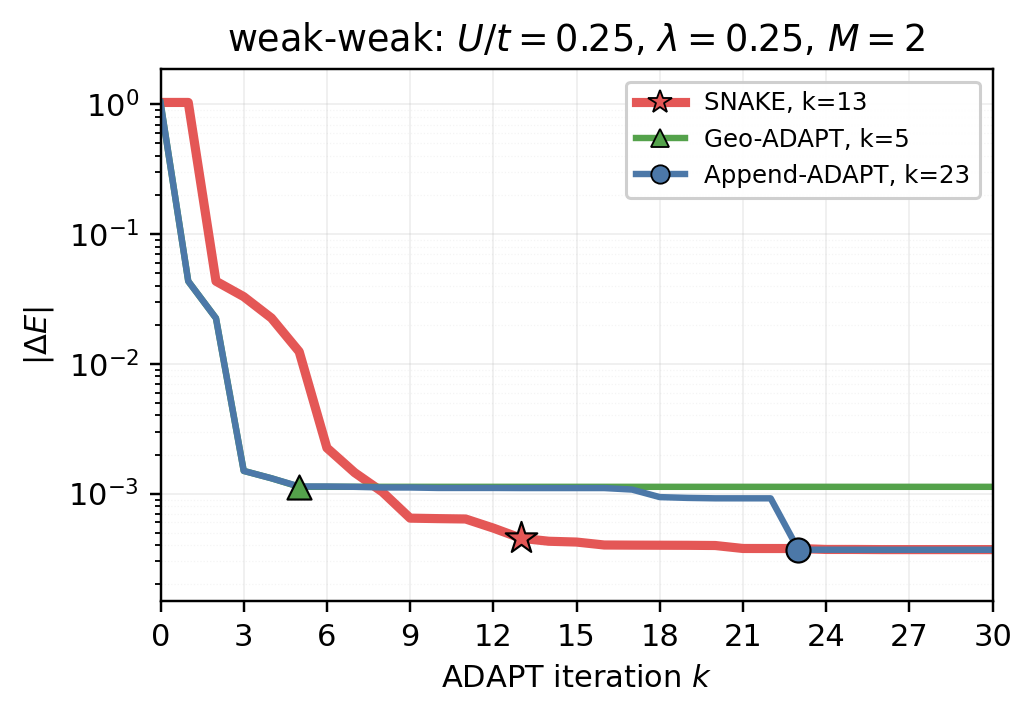
\includegraphics[width=\linewidth]{figures/paper_i_physical_lane_snake_duplicate_20260708/paper_i_physical_lane_snake_duplicate_20260708__weak_weak.png}
\par\smallskip
\begin{tabular*}{\linewidth}{@{}l@{\extracolsep{\fill}}rrrrrr@{}}
\toprule
Method & \(k_{\rm pl}\) & \(|\Delta E|\) & \(N_{\twq}\) & \(D_{\twq}\) & \(D_c\) & \(S\)\\
\midrule
SNAKE & 13 & 4.524e-04 & 48 & 34 & 183 & 5,009 \\
Geo & 5 & 1.312e-03 & 98 & 67 & 480 & 24,859 \\
% Omitted Geo singleton source row: Geo singleton & 5 & 1.312e-03 & -- & 98 & 70 & 539 & 466,828 \\
Append & 23 & 9.193e-04 & 4,216 & 4,033 & 15,936 & 108,633 \\
% Omitted Append singleton source row: Append singleton & 5 & 1.312e-03 & -- & 98 & 70 & 534 & 3,129 \\
\bottomrule
\end{tabular*}
\end{minipage}\hfill
\begin{minipage}[t]{0.322\textwidth}
\centering
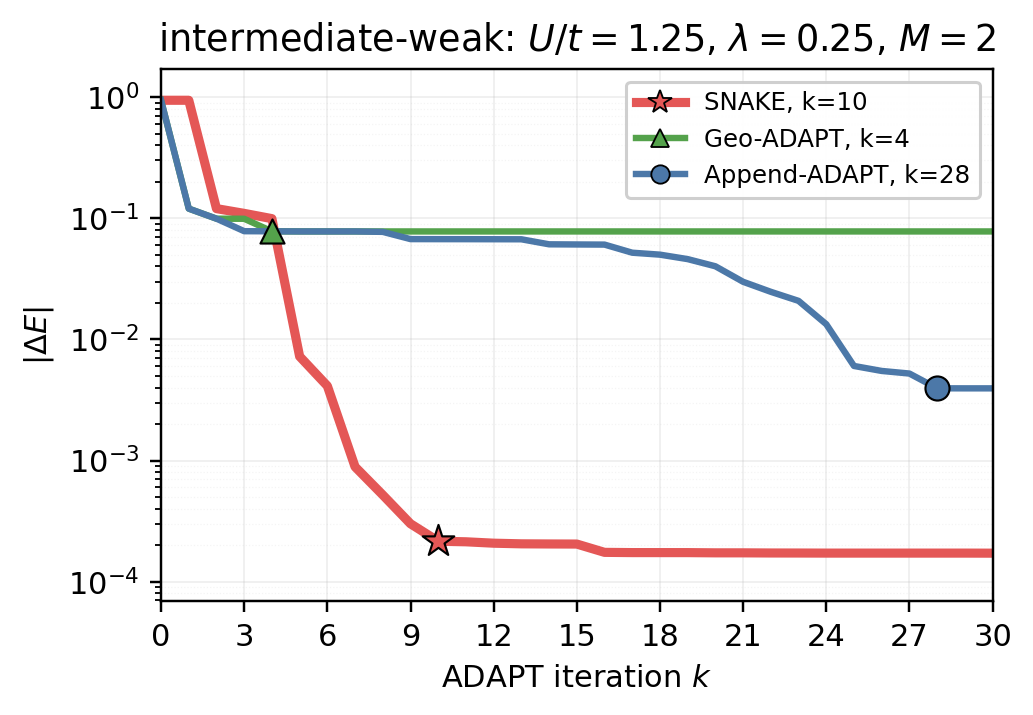
\includegraphics[width=\linewidth]{figures/paper_i_physical_lane_snake_duplicate_20260708/paper_i_physical_lane_snake_duplicate_20260708__intermediate_weak.png}
\par\smallskip
\begin{tabular*}{\linewidth}{@{}l@{\extracolsep{\fill}}rrrrrr@{}}
\toprule
Method & \(k_{\rm pl}\) & \(|\Delta E|\) & \(N_{\twq}\) & \(D_{\twq}\) & \(D_c\) & \(S\)\\
\midrule
SNAKE & 10 & 2.158e-04 & 38 & 30 & 133 & 4,142 \\
Geo & 4 & 9.893e-02 & 70 & 69 & 528 & 19,792 \\
% Omitted Geo singleton source row: Geo singleton & 2 & 0.12 & -- & 40 & 40 & 285 & 186,863 \\
Append & 28 & 5.224e-03 & 4,276 & 4,059 & 15,924 & 231,208 \\
% Omitted Append singleton source row: Append singleton & 23 & 2.277e-02 & -- & 562 & 485 & 2,374 & 134,322 \\
\bottomrule
\end{tabular*}
\end{minipage}\hfill
\begin{minipage}[t]{0.322\textwidth}
\centering
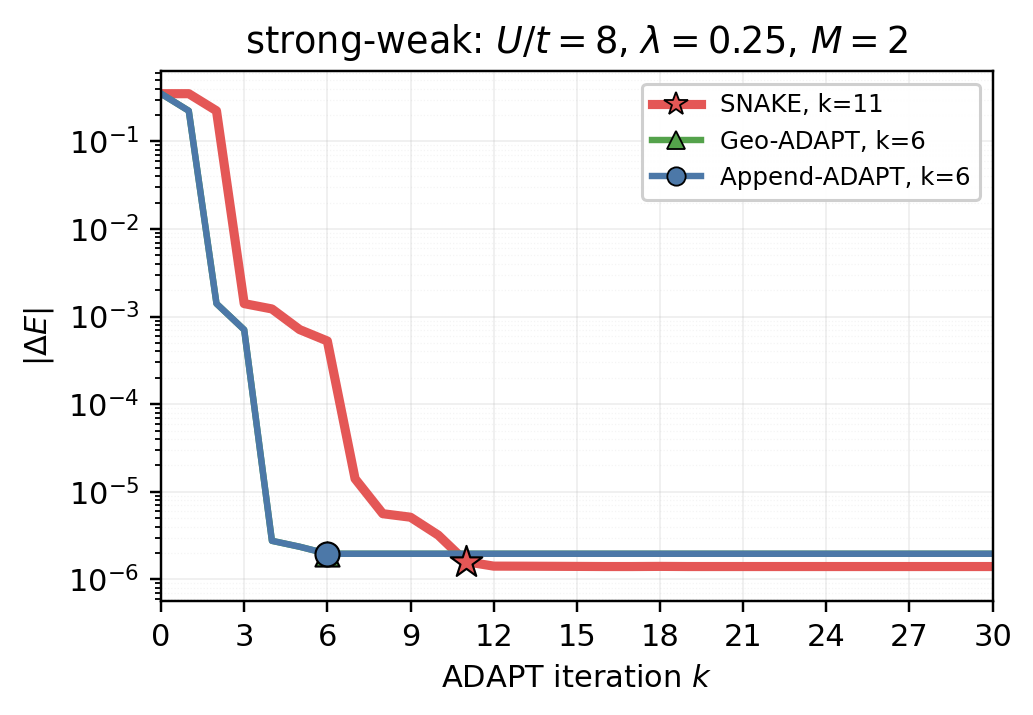
\includegraphics[width=\linewidth]{figures/paper_i_physical_lane_snake_duplicate_20260708/paper_i_physical_lane_snake_duplicate_20260708__strong_weak.png}
\par\smallskip
\begin{tabular*}{\linewidth}{@{}l@{\extracolsep{\fill}}rrrrrr@{}}
\toprule
Method & \(k_{\rm pl}\) & \(|\Delta E|\) & \(N_{\twq}\) & \(D_{\twq}\) & \(D_c\) & \(S\)\\
\midrule
SNAKE & 11 & 1.591e-06 & 44 & 37 & 200 & 4,126 \\
Geo & 6 & 2.355e-06 & 146 & 117 & 763 & 30,007 \\
% Omitted Geo singleton source row: Geo singleton & 4 & 7.064e-04 & -- & 116 & 116 & 710 & 373,478 \\
Append & 6 & 2.355e-06 & 146 & 118 & 762 & 2,137 \\
% Omitted Append singleton source row: Append singleton & 9 & 1.672e-06 & -- & 156 & 126 & 814 & 7,310 \\
\bottomrule
\end{tabular*}
\end{minipage}
\par\bigskip
\begin{minipage}[t]{0.322\textwidth}
\centering
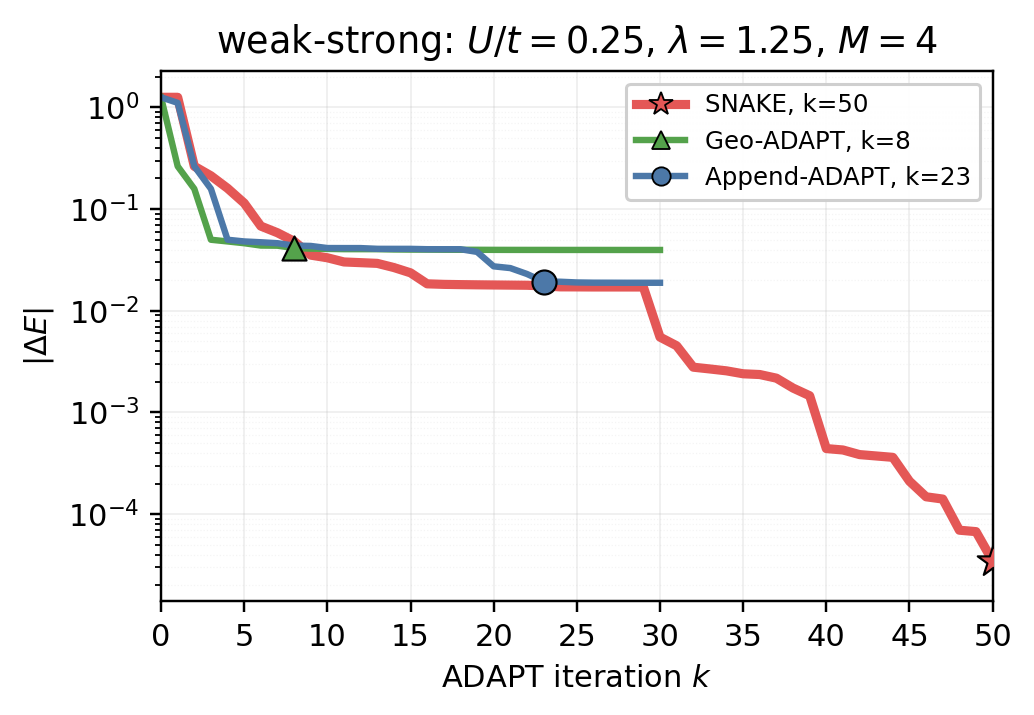
\includegraphics[width=\linewidth]{figures/paper_i_physical_lane_snake_duplicate_20260708/paper_i_physical_lane_snake_duplicate_20260708__weak_strong.png}
\par\smallskip
\begin{tabular*}{\linewidth}{@{}l@{\extracolsep{\fill}}rrrrrr@{}}
\toprule
Method & \(k_{\rm pl}\) & \(|\Delta E|\) & \(N_{\twq}\) & \(D_{\twq}\) & \(D_c\) & \(S\)\\
\midrule
SNAKE & 16 & 1.841e-02 & 70 & 61 & 206 & 17,305 \\
Geo & 8 & 4.365e-02 & 1,784 & 1,641 & 6,160 & 47,155 \\
% Omitted Geo singleton source row: Geo singleton & 4 & 0.157 & -- & 280 & 280 & 1,610 & 2,728,149 \\
Append & 23 & 2.301e-02 & 32,596 & 31,946 & 94,899 & 136,947 \\
% Omitted Append singleton source row: Append singleton & 28 & 3.468e-02 & -- & 27,400 & 27,169 & 77,949 & 228,209 \\
\bottomrule
\end{tabular*}
\end{minipage}\hfill
\begin{minipage}[t]{0.322\textwidth}
\centering
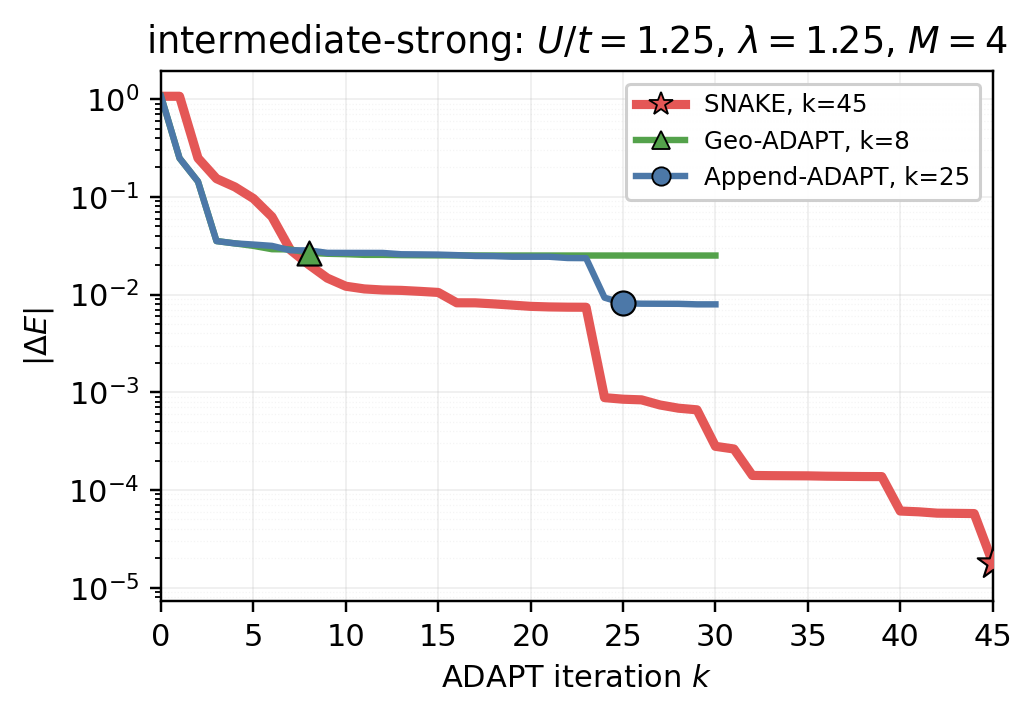
\includegraphics[width=\linewidth]{figures/paper_i_physical_lane_snake_duplicate_20260708/paper_i_physical_lane_snake_duplicate_20260708__intermediate_strong.png}
\par\smallskip
\begin{tabular*}{\linewidth}{@{}l@{\extracolsep{\fill}}rrrrrr@{}}
\toprule
Method & \(k_{\rm pl}\) & \(|\Delta E|\) & \(N_{\twq}\) & \(D_{\twq}\) & \(D_c\) & \(S\)\\
\midrule
SNAKE & 28 & 6.871e-04 & 150 & 121 & 540 & 28,617 \\
Geo & 8 & 2.898e-02 & 1,784 & 1,632 & 6,104 & 47,245 \\
% Omitted Geo singleton source row: Geo singleton & 2 & 0.249 & -- & 40 & 40 & 285 & 1,364,468 \\
Append & 25 & 9.296e-03 & 33,340 & 32,457 & 97,248 & 167,416 \\
% Omitted Append singleton source row: Append singleton & 28 & 1.416e-02 & -- & 32,782 & 32,239 & 96,144 & 247,019 \\
\bottomrule
\end{tabular*}
\end{minipage}\hfill
\begin{minipage}[t]{0.322\textwidth}
\centering
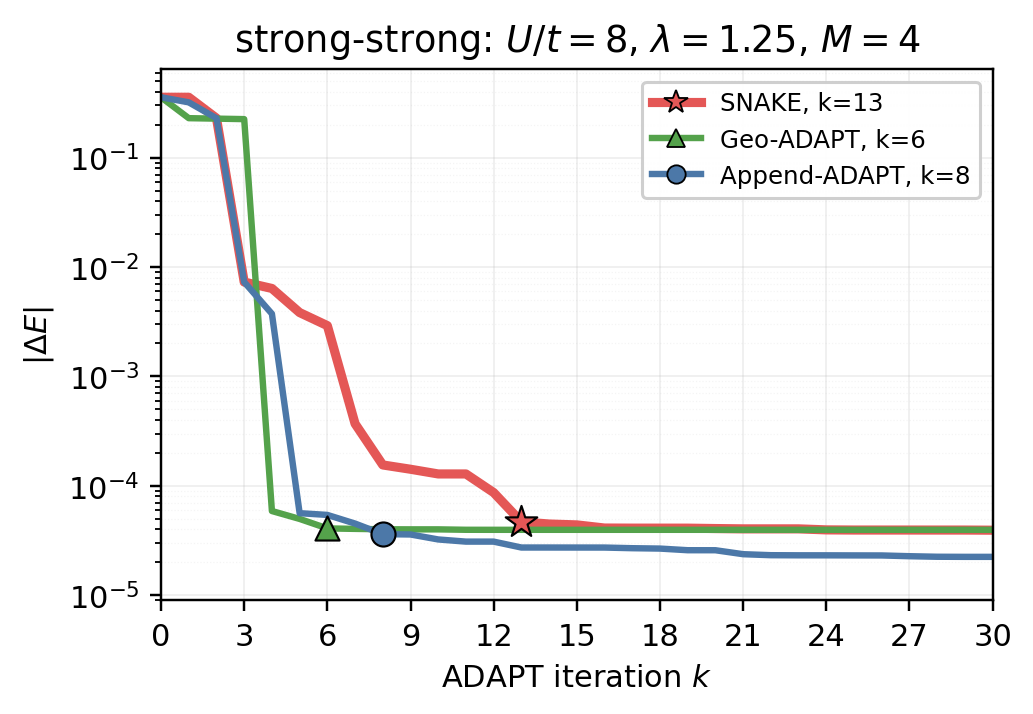
\includegraphics[width=\linewidth]{figures/paper_i_physical_lane_snake_duplicate_20260708/paper_i_physical_lane_snake_duplicate_20260708__strong_strong.png}
\par\smallskip
\begin{tabular*}{\linewidth}{@{}l@{\extracolsep{\fill}}rrrrrr@{}}
\toprule
Method & \(k_{\rm pl}\) & \(|\Delta E|\) & \(N_{\twq}\) & \(D_{\twq}\) & \(D_c\) & \(S\)\\
\midrule
SNAKE & 13 & 4.683e-05 & 48 & 39 & 188 & 5,153 \\
Geo & 6 & 4.982e-05 & 348 & 206 & 1,149 & 33,962 \\
% Omitted Geo singleton source row: Geo singleton & 4 & 3.736e-03 & -- & 208 & 208 & 1,170 & 2,727,920 \\
Append & 8 & 3.616e-05 & 7,976 & 7,833 & 26,219 & 6,378 \\
% Omitted Append singleton source row: Append singleton & 24 & 2.654e-05 & -- & 32,234 & 31,714 & 93,028 & 89,870 \\
\bottomrule
\end{tabular*}
\end{minipage}
\captionof{figure}{Hubbard--Holstein error-versus-iteration trajectories and Qiskit plateau-prefix costs. The top row shows weak-Holstein sectors with \(M=2\), and the bottom row shows strong-Holstein sectors with \(M=4\). Markers indicate the reported plateau prefix \(k_{\rm pl}\); mini-tables report the corresponding energy error, compiled two-qubit gate count \(N_{\twq}\), two-qubit depth \(D_{\twq}\), compiled depth \(D_c\), and logical estimator-query count \(S\).}
\label{fig:hh_main_results_composite}
\end{center}
\end{minipage}
\clearpage
\twocolumngrid
\par\addvspace{0.45ex}
% BEGIN_DRAFT_HH_CHILD_FAIRNESS_PROSE_TODO_20260624
% Condensed future-prose note; comment only, do not render yet.
% Use the native-forced SPSA Pauli-child protocol as the main displayed HH comparison.
% Treat monotone/non-forced rows as sensitivity evidence: Append and Geo improve under monotone,
% while SNAKE is stronger in the native-forced child+Schur condition or comparable to monotone.
% No-child SNAKE hurts under the current parameterization; phrase this as a hyperparameter/
% Optuna/settings limitation, not as an intrinsic limitation of SNAKE.
% Schur warm-start versus no-Schur warm-start did not materially change same-cutoff
% energy error in this comparison; treat Schur as a refit/conditioning and cost-shaping
% mechanism unless a later source-locked replay shows an accuracy separation.
% Candidate claim: native-forced SNAKE child+Schur versus Geo monotone no-child gives
% same-order aggregate same-cutoff energy accuracy with much smaller SNAKE compiled circuit cost.
% Shot/work costs remain pending under a common accounting convention.
% Avoid overclaiming: strong--weak is the visible outlier in the compact comparison.
% Source support: output/pdf/paper_i_hh_child_fairness_20260623/
% paper_i_hh_child_fairness_compact_child_schur_20260623.{pdf,json,csv}.
% END_DRAFT_HH_CHILD_FAIRNESS_PROSE_TODO_20260624
\par\addvspace{1.0ex}

% BEGIN_MACHINE_READABLE_WEAK_WEAK_SNAKE_MECHANISM_ABLATION_TERMINAL_METRICS_20260709
% {"schema":"paper_i_weak_weak_snake_mechanism_ablation_terminal_delta_metrics_v4","updated_date":"2026-07-09","table_labels":["tab:weak_weak_snake_mechanism_ablation_terminal_metrics"],"support_pdf":"output/pdf/paper_i_hh_weak_weak_snake_mechanism_ablation_20260708/paper_i_hh_weak_weak_snake_mechanism_ablation_20260708.pdf","support_json":"output/pdf/paper_i_hh_weak_weak_snake_mechanism_ablation_20260708/paper_i_hh_weak_weak_snake_mechanism_ablation_20260708.json","support_json_sha256":"07304f5bec8b71f8bf3ce29b2f1613899d74937e889af78cfcdfaf859f1630f6","source_table_page":"support PDF page 7, terminal-iteration metrics promoted as delta-from-anchor table","row_policy":"source-anchor row omitted because all deltas are zero; no-shortlisting omitted; Status column omitted; batch-cap rows omitted pending corrected batching audit because audited batch-cap trajectories did not admit multi-record batches","benchmark":"weak--weak Hubbard--Holstein","optimizer":"POWELL","terminal_depth_contract":"terminal iteration-prefix deltas at k=30 relative to Source anchor; k column omitted from rendered table","rounding_policy":"Delta energy-error percent rounded to integer except no-batching, no-prune, no-cost-term, and no-novelty rows keep one decimal place"}
% END_MACHINE_READABLE_WEAK_WEAK_SNAKE_MECHANISM_ABLATION_TERMINAL_METRICS_20260709
\noindent\begin{minipage}{\columnwidth}
\captionof{table}{\label{tab:weak_weak_snake_mechanism_ablation_terminal_metrics}Weak--weak Hubbard--Holstein SNAKE mechanism ablations at the terminal 30-iteration prefix. Entries are differences from the source anchor in the terminal-iteration support table; the source-anchor row is omitted because all deltas are zero. Here \(d\) is the number of generators in the terminal ansatz. The energy-error column is a percent change, while circuit-resource and estimator-work columns are absolute integer deltas. \(\Delta S\) is computed from terminal branch-local \(S_{\rm alg}\). Batch-cap rows are omitted pending a corrected batching audit.}
\centering
\scriptsize
\setlength{\tabcolsep}{1.2pt}
\renewcommand{\arraystretch}{1.02}
\resizebox{\columnwidth}{!}{%
\begin{tabular}{@{}lrrrrrr@{}}
\toprule
Variant & $\Delta|\Delta E|$ (\%) & $\Delta d$ & $\Delta N_{\twq}$ & $\Delta D_{\twq}$ & $\Delta D_c$ & $\Delta S$ \\
\midrule
No batching reference & 1.0 & 0 & -2 & -12 & -67 & -271 \\
No prune & 1.3 & 10 & 34 & 23 & 116 & 706 \\
No cost term & 1.4 & -2 & -6 & -12 & -52 & 574 \\
No novelty & 1.1 & -2 & -2 & -3 & -58 & -3198 \\
Novelty only; no second order & 202 & -10 & 166 & 112 & 922 & 34119 \\
Second order only; no novelty & 202 & -8 & 562 & 499 & 2619 & 55576 \\
No Phase 3 & 202 & -10 & 114 & 59 & 550 & 40823 \\
Phase 1 only; macro pool & 202 & -12 & 182 & 117 & 883 & 26538 \\
Phase 1 only; singleton pool & 202 & -5 & 24 & 15 & 229 & 19949 \\
Full geometry window & 8 & -1 & -10 & -16 & -88 & -530 \\
\bottomrule
\end{tabular}%
}
\end{minipage}
\par\addvspace{1.0ex}

\section{Discussion and conclusion}
\label{sec:discussion}
\label{sec:conclusion}

% Struct label: Mechanistic interpretation
SNAKE's second-order model combines the Fubini--Study metric with Schur-complement treatment of coupling between candidate directions and refit-coordinate windows, enabling more accurate candidate-generator ranking with respect to expected energy reduction. This accuracy produces more efficient energy-minimizing state trajectories, reducing hardware costs such as gate count and the shot-count proxy. In addition, SNAKE rewards generator-induced novel tangent directions, expanding the accessible state manifold while avoiding generator redundancy. Although this increases the variational landscape, it can reduce the effective parameter dimension and improve linear independence, both of which can support parameter-update convergence. Generators are further down-weighted when they induce disproportionate circuit burden.

This efficiency, combined with shot-attenuating mechanisms such as shortlisting and geometry-aware batching policies, further facilitates shot-proxy reduction, while beam continuation explores near-degenerate choices without increasing the per-branch resource burden. Generator ablation further reduces persistent circuit cost when selected operators become locally recoverable from the remaining ansatz.

% Struct label: Scope and limitations
Despite targeting NISQ-era constraints, the present results are noiseless and use small, classically solvable two-site models. Further work should compare noise models and noise-aware stopping criteria for ADAPT algorithms. Finite-shot confidence envelopes, backend-resolution floors, iteration-dependent gate-selection breadth and mechanistic pressures, and rolling batching, Schur-refit, and geometry windows selected by coordinate-coupling-strength history remain prospective SNAKE extensions. Further work may focus on lane partitioning in shortlists and pruning behavior based on the physical process the operator encodes, such as UCCSD vs a polaronic operator.
% Struct label: Summary/so what
Variational quantum eigensolvers remain an important approach for simulating physical systems on near-term quantum hardware. SNAKE extends ADAPT-VQE by explicitly incorporating state geometry, measurement burden, and hardware constraints into generator selection. Across the benchmark systems studied here, this produces more accurate or more resource-efficient ansatz prefixes than existing adaptive comparators, including for mixed fermion--boson systems. The Hubbard--Holstein operator pool is defined by the physical lanes in Sec.~\ref{subsec:hh_physical_operator_lanes}, with the spin-boson/Rabi pool defined in Appendix~\ref{app:spin_boson_rabi}.

\appendix

\section{Total estimator-query accounting}
\label{app:estimator_queries}

The \(S\) column in the Hubbard, spin-boson/Rabi, and Hubbard--Holstein reported tables gives a displayed-prefix logical scalar estimator-query count. One query is one scalar expectation-value primitive used by the algorithm at the relevant prepared state, such as a candidate-gradient scalar, a Fubini--Study norm scalar, a Gram/metric entry, a curvature/Hessian/coupling entry, or one Hamiltonian objective evaluation in an optimizer/refit. Algebraic recombination, ranking, pseudoinverse solves, Schur complements, and other classical postprocessing are not additional queries. Same-state reuse and symmetry are applied: a scalar primitive reused by multiple formulas at the same prepared state is counted once, and symmetric matrix entries are counted once. The same primitive evaluated at a different accepted-prefix state or optimizer/refit trial state counts again. Thus \(S\) is not a physical-shot count, raw Pauli-word count, or post-Pauli-grouped measurement-setting count.

Let \(k\) index accepted adaptive iterations, and let \(k_{\rm pl}\) be the displayed plateau-prefix iteration. For append-only ADAPT, let \(\mathcal A_k\) be the live candidate set scored before the \(k\)-th admission, with \(n_k=|\mathcal A_k|\). The candidate-gradient scan contributes \(n_k\). For Geo-ADAPT, the tangents \(\tau_r^{(k)}=(I-|\psi_k\rangle\langle\psi_k|)(-iA_r|\psi_k\rangle)\) define \(G_{rs}^{(k)}=\Re\langle\tau_r^{(k)},\tau_s^{(k)}\rangle\) for \(r,s\in\mathcal A_k\), adding \(n_k(n_k+1)/2\) symmetric metric-entry queries. If \(f_k\) is the number of Hamiltonian objective evaluations used by the refit optimizer after the \(k\)-th admission, then
\begin{equation*}
\begin{aligned}
S_{\rm ADAPT}
&=
\sum_{k=0}^{k_{\rm pl}}
\left(n_k+f_k\right),
\\
S_{\rm Geo}
&=
\sum_{k=0}^{k_{\rm pl}}
\left(n_k+\frac{n_k(n_k+1)}{2}+f_k\right).
\end{aligned}
% source label: eq:appendix_s_adapt_geo
\end{equation*}

For SNAKE, let \(P_\ell(k)\), with \(\ell=0,1,2,3\), denote the scalar-primitive sets requested or made available by Phase \(\ell\) before the \(k\)-th admission, before de-duplication against earlier phases. If \(f_k\) is the number of Hamiltonian objective evaluations used by the optimizer and refit checks after the \(k\)-th admission, then
\begin{align}
S_{\rm SNAKE}
&=
\sum_{k=0}^{k_{\rm pl}}
\left[
|P_0(k)|+|P_1(k)\setminus P_0(k)|
\right.
\nonumber\\
&\qquad\left.
 +|P_2(k)\setminus(P_0(k)\cup P_1(k))|
\right.
\nonumber\\
&\qquad\left.
 +|P_3(k)\setminus(P_0(k)\cup P_1(k)\cup P_2(k))|
+f_k
\right].
\label{eq:appendix_s_snake}
\end{align}

The set subtractions in Eq.~\eqref{eq:appendix_s_snake} implement same-prefix reuse across phases. Pauli decompositions, compatible-Pauli grouping, shot allocation, and grouped measurement settings are lower-level measurement diagnostics and are not resolved in the reported \(S\) column; they enter only through hardware/measurement-cost proxies or separately labeled grouped-shot diagnostics.

\section{SNAKE benchmark configuration}
\label{app:results_discussion}

The reported Hubbard--Holstein SNAKE rows use a common algorithmic
configuration across interaction regimes. Hamiltonian parameters, phonon
cutoff, reference state, plateau prefix, and compiled costs are reported with
the corresponding result rows. This appendix records the non-Hamiltonian
settings needed to interpret those rows: staged shortlisting, physical-lane
retention, Pauli-child splitting, resource penalties, geometry windows,
batching and beam policy, generator ablation, and inner refit convention.
Appendix~\ref{app:estimator_queries} defines the total-estimator-query
accounting for the \(S\) column, and Appendix~\ref{app:spsa_settings} records
the SPSA optimizer schedule used by SPSA-based diagnostic and comparator
records.

% Source support:
% output/pdf/paper_i_hh_snake_canonical_appendix_settings_20260709/
% paper_i_hh_snake_canonical_appendix_settings_20260709.{pdf,tex,csv,json}
\begin{widetext}
\captionof{table}{\label{tab:snake_benchmark_configuration}Common
Hubbard--Holstein SNAKE algorithmic configuration used for the reported SNAKE
rows unless a row explicitly states that it is a diagnostic exception.}
\centering
\scriptsize
\setlength{\tabcolsep}{2.2pt}
\renewcommand{\arraystretch}{1.08}
\resizebox{\textwidth}{!}{%
\begin{tabular}{@{}p{0.20\textwidth}p{0.24\textwidth}p{0.50\textwidth}@{}}
\toprule
Component & Symbol or quantity & Value used \\
\midrule
Encoding & fermion and phonon encoding & blocked Jordan--Wigner fermions; binary phonon registers; open boundary conditions \\
Cutoff-dependent pool surface & \(M=2\), \(M=4\) & \(M=2\): 2 boson bits/site, 8 qubits, 9 legal boson codewords, \(|\mathcal G|=97\); \(M=4\): 3 boson bits/site, 10 qubits, 25 legal boson codewords, \(|\mathcal G|=103\) \\
Physical lanes & \(\lambda:\mathcal G\to\mathcal L\) & six physical operator-type lanes: electronic UCCSD, electronic hopping/current, phonon cloud, phonon relaxation, dressed electron--phonon, and Hamiltonian-block rotations \\
Insertion positions & \(\mathcal P_k\) & at most 6 candidate insertion positions are probed \\
Shortlist caps & \(N_1,N_2,N_3\) & \(N_1=8\), \(N_2=4\), \(N_3=4\) \\
Lane live-test threshold & Eq.~\eqref{eq:phase_restriction_map}, \(\tau_t\) & a lane remains live when \(S^{(t)}(r_\ell^\star)\ge \tau_t S^{(t)}(r_{\mathcal L}^\star)\); the Hubbard--Holstein rows use \(\tau_2=0.10\) \\
Pauli-child splitting & \(A_J,\Gamma(A_J)\) & singleton Pauli-child splitting, \(|J|\le 1\); hard fermion-sector guard with \(\epsilon=10^{-10}\) \\
Resource penalty & \(K_t(r)\) & Phase-I weights \((\lambda_{\twq},\lambda_d,\lambda_{1q},\lambda_\theta,\lambda_{\rm shot})=(0.05,0.05,0.025,0,0.02)\); Phase-II/III weights \((0.20,0.20,0.10,0.10,0.15)\) \\
Estimator-query proxy & \(S\), \(\sigma_\star\) & one logical estimator-query unit per active phase; \(\sigma_\star=1\) \\
Trust-region scale & \(\rho,\lambda_F\) & \(\rho=0.25\), \(\lambda_F=1.0\); trust-region score mode \\
Regularization & metric, score, and Schur floors & metric floor \(10^{-12}\); cheap-score floor \(10^{-12}\); \(\lambda_H=10^{-6}\); ridge growth factor 10 for at most 12 steps \\
Geometry window & \(W_r\) & fixed local geometry window size 99, which is larger than the ansatz lengths in these rows and therefore gives full-ansatz geometry \\
Batching & \(\mathcal B_k\) & Phase-II and Phase-III batching disabled; effective \(|\mathcal B_k|=1\) \\
Beam retention & \(B_{\rm live},B_{\rm child},\lambda_{\rm beam}\) & \(B_{\rm live}=3\), \(B_{\rm child}=2\), \(\lambda_{\rm beam}=0.005\) \\
Generator ablation & \(\mathcal D_k\) & enabled; recoverability-ladder policy; prune mode both \\
Ablation eligibility & \(\tilde p,\tilde c\) & protection steps \(\tilde p=2\); cooldown steps \(\tilde c=2\); checkpoint period 3; local prune window 4 \\
Schur prune nomination & \(\eta\) & metric-regularized Schur nomination active with \(\eta=0.01\); stationary-\(G_W\)-zero solve mode; ansatz-entry denominator cost weighting \\
Ablation acceptance & rollback tolerances & max regression \(10^{-8}\); small-\(\theta\) absolute threshold \(10^{-3}\); small-\(\theta\) relative threshold \(0.5\); retained-gain ratio \(0.5\); tolerance-screen coefficient \(0.01\) \\
Inner optimizer & Eq.~\eqref{eq:theta_opt} & Powell optimizer; maxiter 200; no separate maxfev cap; final refit maxiter 200 \\
Refit policy & active ansatz window & full ansatz refit every iteration; no eight-iteration local-window cadence \\
Stopping and reporting & \(k_{\max},k_{\rm pl}\) & run horizon is row-specific; reported values use the displayed plateau prefix \(k_{\rm pl}\) \\
\bottomrule
\end{tabular}%
}
\end{widetext}

\section{Simulated Noise Results}
\label{app:noise_selection_robustness}
\label{app:finite_shot_score_robustness}

% BEGIN_MACHINE_READABLE_SNAKE_NOISE_ROBUSTNESS_PROMOTED_20260608
% {
%   "schema": "paper_i_snake_noise_robustness_appendix_evidence_v3",
%   "updated_date": "2026-06-08",
%   "table_or_section_label": "app:noise_selection_robustness",
%   "legacy_section_label": "app:finite_shot_score_robustness",
%   "claim_status": "promoted_appendix_diagnostic_evidence",
%   "method": "SNAKE",
%   "target_abs_delta_e_reference": 0.0002,
%   "scalar_value_noise_evidence": {
%     "benchmark_family": "Hubbard-Holstein",
%     "regime": "strong-weak",
%     "noise_surface": "scalar_post_expectation_value_noise",
%     "noise_model": "gaussian_iid_v1",
%     "n_eff_note": "N_eff is the scalar value-noise model knob in std_E=sigma0_abs/sqrt(N_eff), not a physical hardware shot count.",
%     "n_eff": 1000000000000000000,
%     "sigma0_abs": 0.001,
%     "std_E": 1e-12,
%     "same_noise_noise_floor_result_json": "output/diagnostics/hh_sw_shot_proxy_noise_floor_neff1000000000000000000_20260607/shot_proxy_noise_floor_stop/run/hh_L2_nph2_three_model_sym_strong_weak/trial_0000/hh_L2_nph2_three_model_sym_strong_weak/json/result.json",
%     "same_noise_noise_floor_records_tsv": "output/diagnostics/hh_sw_shot_proxy_noise_floor_neff1000000000000000000_20260607/records/paper_i_hh_noise_robustness_records.tsv",
%     "same_noise_noise_floor_audit_json": "output/diagnostics/hh_sw_shot_proxy_noise_floor_neff1000000000000000000_20260607/shot_proxy_noise_floor_stop/source_lock_audit.json",
%     "same_noise_noise_floor_stop_reason": "benchmark_abs_delta_e_target",
%     "same_noise_noise_floor_depth": 16,
%     "same_noise_noise_floor_energy": -0.4948070750781848,
%     "same_noise_noise_floor_abs_delta_e": 0.0001885640305164804,
%     "same_noise_noise_floor_benchmark_current_error": 0.000198427500580467,
%     "same_noise_noise_floor_target_hit_success": true,
%     "same_noise_noise_floor_source_lock_audit_status": "pass",
%     "same_noise_confidence_result_json": "output/diagnostics/hh_sw_shot_proxy_confidence_neff1000000000000000000_20260607/shot_proxy_confidence_scoring/run/hh_L2_nph2_three_model_sym_strong_weak/trial_0000/hh_L2_nph2_three_model_sym_strong_weak/json/result.json",
%     "same_noise_confidence_records_tsv": "output/diagnostics/hh_sw_shot_proxy_confidence_neff1000000000000000000_20260607/records/paper_i_hh_noise_robustness_records.tsv",
%     "same_noise_confidence_audit_json": "output/diagnostics/hh_sw_shot_proxy_confidence_neff1000000000000000000_20260607/shot_proxy_confidence_scoring/source_lock_audit.json",
%     "same_noise_confidence_phase1_score_z_alpha": 1.0,
%     "same_noise_confidence_phase2_score_z_alpha": 1.0,
%     "same_noise_confidence_stop_reason": "benchmark_abs_delta_e_target",
%     "same_noise_confidence_depth": 16,
%     "same_noise_confidence_energy": -0.4948070750781848,
%     "same_noise_confidence_abs_delta_e": 0.0001885640305164804,
%     "same_noise_confidence_benchmark_current_error": 0.000198427500580467,
%     "same_noise_confidence_target_hit_success": true,
%     "local_noiseless_baseline_result_json": "output/diagnostics/hh_sw_trial0011_oracle_original_route_pair_20260601/ideal_oracle_original_route/result.json",
%     "local_noiseless_baseline_depth": 13,
%     "local_noiseless_baseline_abs_delta_e": 0.0001775162084057813,
%     "proxy_summary_json": "output/diagnostics/hh_sw_noise_proxy_mapping_20260607/summary.json",
%     "local_noiseless_baseline_S_norm": 40269,
%     "same_noise_noise_floor_S_norm": 56745,
%     "same_noise_noise_floor_S_norm_factor_vs_baseline": 1.4091484764955673
%   },
%   "combined_scalar_and_gate_noise_evidence": {
%     "benchmark_family": "Hubbard",
%     "regime": "strong",
%     "noise_surface": "scalar_value_noise_plus_synthetic_depolarizing_expectation_surface",
%     "phase3_oracle_gradient_mode": "aer_density_matrix_synthetic_depolarizing",
%     "phase3_oracle_execution_surface": "expectation_v1",
%     "phase3_oracle_inner_objective_mode": "noisy_v1",
%     "scalar_value_noise_model": "gaussian_iid_v1",
%     "n_eff_note": "N_eff is the scalar value-noise model knob in std_E=sigma0_abs/sqrt(N_eff), not a physical hardware shot count.",
%     "n_eff": 200,
%     "sigma0_abs": 0.001,
%     "std_E": 7.071067811865475e-05,
%     "phase3_oracle_synthetic_depolarizing_1q_error": 1e-6,
%     "phase3_oracle_synthetic_depolarizing_2q_error": 1e-5,
%     "phase3_oracle_synthetic_depolarizing_1q_gates": "x sx rx ry h",
%     "phase3_oracle_synthetic_depolarizing_2q_gates": "cx cz ecr",
%     "rollback_mode": "off",
%     "target_stop_policy": "disabled_for_fixed_iteration_diagnostic",
%     "fixed_depth_cap": 16,
%     "retrieval_status": "manual_stop_after_iteration6_checkpoint",
%     "remote_runner_run_id": "20260608T184045Z-2bbb85e1",
%     "retrieved_checkpoint_json": "output/diagnostics/hubbard_strong_snake_gate_fixed_depth_20260608/hubbard_strong_combined_scalar_neff200_p1q1em6_p2q1em5_rollbackoff_fixed_depth16_remote_v1/stopped_or_exit_retrieved_current_combined_neff200_p1q1em6_p2q1em5_rollbackoff_fixed_depth_diagnostic_20260608.json",
%     "retrieved_checkpoint_sha256": "cdc754a92afacc18bea32abcec0c761e7faef8131b0876af7c8071b864f9deeb",
%     "retrieved_checkpoint_schema_version": "static_adapt_current_checkpoint_v1",
%     "retrieved_checkpoint_depth": 6,
%     "retrieved_checkpoint_ansatz_depth": 6,
%     "retrieved_checkpoint_energy": -1.3862596416086974,
%     "retrieved_checkpoint_abs_delta_e": 0.0002587052793157074,
%     "best_recorded_depth": 5,
%     "best_recorded_abs_delta_e": 0.00025163740705380633,
%     "best_recorded_energy": -1.3862525737364355,
%     "depth_error_history": [
%       {"depth": 1, "abs_delta_e": 0.8857512517253792, "energy": -0.5002496846040025},
%       {"depth": 2, "abs_delta_e": 0.13578550228745456, "energy": -1.2502154340419271},
%       {"depth": 3, "abs_delta_e": 0.00025808240219249434, "energy": -1.3862590187315742},
%       {"depth": 4, "abs_delta_e": 0.0002817046409628876, "energy": -1.3862826409703446},
%       {"depth": 5, "abs_delta_e": 0.00025163740705380633, "energy": -1.3862525737364355},
%       {"depth": 6, "abs_delta_e": 0.0002587052793157074, "energy": -1.3862596416086974}
%     ],
%     "result_json": null,
%     "result_json_note": "No final result.json was expected because the fixed-iteration diagnostic was intentionally stopped after a recoverable iteration-6 checkpoint."
%   },
%   "limitations": [
%     "The Hubbard-Holstein scalar value-noise evidence uses N_eff as an internal scalar value-noise knob, not a physical hardware shot count.",
%     "The promoted combined-noise diagnostic is a fast Hubbard surrogate for SNAKE robustness under simultaneous scalar value noise and synthetic one-/two-qubit depolarizing expectation-surface noise.",
%     "The synthetic depolarizing surface is an AER density-matrix diagnostic rather than calibrated hardware noise."
%   ]
% }
% END_MACHINE_READABLE_SNAKE_NOISE_ROBUSTNESS_PROMOTED_20260608

% BEGIN_MACHINE_READABLE_HUBBARD_FULL_NOISE_FIXED_DEPTH8_SWEEP_20260613
% {"schema":"paper_i_hubbard_full_noise_fixed_depth8_appendix_pointer_v2","updated_date":"2026-06-14","support_md":"MATH/paper_facing/paper_I_static_scaffold/hubbard_full_noise_fixed_depth8_support_20260613.md","support_md_sha256":"7e4f39fa8fc5022020e87f0978c0c23bf6d482691aecda2325ae962aa63a74a6","summary_json":"MATH/paper_facing/paper_I_static_scaffold/hubbard_full_noise_fixed_depth8_summary_20260613.json","summary_json_sha256":"9f4145a66f6a9b09b318eefe5bbd7259c5108b16a85862fb606bea605e0f8af4","source_archive":"output/diagnostics/hubbard_full_noise_sweep_fixed_depth_20260612_v3/hubbard_full_noise_fixed_depth_20260612_v3_results.tgz","source_archive_sha256":"ba3eb9554b1f94c33523b74b82ac9dd716cf710fd1f7d55d2be6eee74f4dbda3","weak_figure_png":"MATH/paper_details/figures/hubbard_weak_full_noise_fixed_depth8_error_vs_iteration_20260613.png","weak_figure_png_sha256":"4e4256c648ee157d421f6358469c9cb6da85f6f3eab17ff3cf75eb1b913e9805","intermediate_figure_png":"MATH/paper_details/figures/hubbard_intermediate_full_noise_fixed_depth8_error_vs_iteration_20260613.png","intermediate_figure_png_sha256":"993c2db10fcb9cfa4918e4a0c0de3f6f46c8fbf6d34969627f00838a1276931e","strong_figure_png":"MATH/paper_details/figures/hubbard_strong_full_noise_fixed_depth8_error_vs_iteration_20260613.png","strong_figure_png_sha256":"50b274802fdca607aeb3241f4fa8a7ce134c4cd10315a28628039d3686c7da75","plot_script":"MATH/paper_facing/paper_I_static_scaffold/plot_hubbard_full_noise_fixed_depth8_20260613.py","plot_script_sha256":"7016c466aacceedd8ff12ccfd7d83344da495faa5e70c7a8314ca1809279810a","fixed_depth":8,"result_count":18,"regimes":["weak U/t=0.5","intermediate U/t=1.5","strong U/t=8"],"displayed_regimes":["weak U/t=0.5","strong U/t=8"],"noise_surfaces":["scalar Gaussian post-expectation value noise","synthetic one-/two-qubit depolarizing expectation-surface noise","frozen coherent overrotation noise"],"gradient_se_backend_stop":"not enabled","plot_policy":"energy error versus ADAPT iteration; color and marker shape encode the noise regime; iteration-8 recoverable frontier branch; ordinary terminal winner branch not used"}
% END_MACHINE_READABLE_HUBBARD_FULL_NOISE_FIXED_DEPTH8_SWEEP_20260613

The finite-noise diagnostics perturb the energy surface used by SNAKE during
candidate scoring and refit. We define the unperturbed reference first. Here
\(\ket{\psi_{\rm ref}}\) is the benchmark reference state, \(\rho_{\rm ref}\)
is its density matrix, \(H\) is the benchmark Hamiltonian, \(k\) is the accepted
ADAPT iteration, \(U_k(\boldsymbol{\theta})\) is the corresponding parameterized
ansatz circuit, and \(\boldsymbol{\theta}\) is its parameter vector. The
noiseless circuit state is \(\rho_k(\boldsymbol{\theta})\), and the noiseless
selected-energy objective is \(E_k(\boldsymbol{\theta})\):
\begin{equation*}
\begin{aligned}
\rho_{\rm ref}
&=\ket{\psi_{\rm ref}}\bra{\psi_{\rm ref}},
\\
\rho_k(\boldsymbol{\theta})
&=U_k(\boldsymbol{\theta})\rho_{\rm ref}U_k^\dagger(\boldsymbol{\theta}),
\\
E_k(\boldsymbol{\theta})
&=\operatorname{Tr}\!\left[H\rho_k(\boldsymbol{\theta})\right].
\end{aligned}
\end{equation*}
The synthetic gate-noise diagnostic replaces each ideal compiled gate by a
noisy gate map. Let \(q\in\{1,2\}\) denote whether the compiled gate acts on one
or two qubits, let \(p_q\) be the corresponding depolarizing probability, and
let \(I_{2^q}\) be the identity on the gate-local \(q\)-qubit Hilbert space. A
\(q\)-qubit depolarizing channel acting on a gate-local density operator
\(\rho\) is
\begin{equation*}
\mathcal D_{p_q}(\rho)
=(1-p_q)\rho+p_q\frac{I_{2^q}}{2^q},
\qquad
q\in\{1,2\}.
\end{equation*}
For a compiled gate instance indexed by \(g\), \(U_g\) is the ideal gate unitary
and \(\mathcal M_g\) is the noisy map obtained by applying the ideal gate and
then the gate-local depolarizing channel with \(p_q=p_1\) for one-qubit gates
and \(p_q=p_2\) for two-qubit gates:
\begin{equation*}
\mathcal M_g(\rho)
=
\mathcal D_{p_q}\!\left(U_g\rho U_g^\dagger\right).
\end{equation*}
In the coherent-overrotation diagnostic, each compiled gate \(U_g\) is preceded
by a small unitary perturbation \(V_g=\exp(-i\delta_gB_g/2)\), where \(B_g\) is
the Hermitian generator for the gate-local overrotation axis and \(\delta_g\) is
the sampled overrotation angle for gate instance \(g\). The angles \(\delta_g\)
are drawn once and held fixed during selection and refit. At accepted ADAPT
iteration \(k\), let \(L_k\) be the number of compiled gate maps in the
corresponding noisy circuit, ordered from input to output. The noisy circuit
state is then the channel composition applied to \(\rho_{\rm ref}\):
\begin{equation*}
\begin{aligned}
\widetilde\rho_k(\boldsymbol{\theta})
&=
\left(\mathcal M_{L_k}\circ\cdots\circ\mathcal M_1\right)
\!\left(\rho_{\rm ref}\right),
\\
\widetilde E_k(\boldsymbol{\theta})
&=
\operatorname{Tr}\!\left[
H\widetilde\rho_k(\boldsymbol{\theta})
\right]
+\xi,
\qquad
\xi\sim\mathcal N(0,\sigma_E^2).
\end{aligned}
\end{equation*}
Here \(\widetilde\rho_k(\boldsymbol{\theta})\) is the noisy circuit state,
\(\widetilde E_k(\boldsymbol{\theta})\) is the noisy scalar objective, and
\(\xi\) is an independent Gaussian value-noise draw added after the Hamiltonian
expectation is evaluated. The scalar width \(\sigma_E\) is an uncalibrated
energy-noise scale; when an effective value-noise size is reported, it is used
only through \(\sigma_E=\sigma_0/\sqrt{N_{\rm eff}}\), where \(\sigma_0\) is a
reference scalar-noise scale and \(N_{\rm eff}\) is an effective value-noise
parameter rather than a physical shot count.

The diagnostics below use fixed-iteration Hubbard SNAKE sweeps under simultaneous scalar value noise, synthetic depolarizing gate noise, and frozen coherent overrotation noise. The curves report absolute energy error for fixed iteration-8 adaptive prefixes; branches that terminate before iteration 8 are excluded from these panels. The displayed weak \((U/t=0.5)\) and strong-Hubbard \((U/t=8)\) panels bracket the interaction range used for this appendix diagnostic. For all curves, the legend level denotes the tuple \((\sigma_E,p_1,p_2,\epsilon_1,\epsilon_2)\), with numerical levels given in Table~\ref{tab:hubbard_noise_levels}.

\noindent\begin{minipage}{\columnwidth}
\begin{center}
\scriptsize
\setlength{\tabcolsep}{2.2pt}
\renewcommand{\arraystretch}{1.05}
\captionof{table}{Noise levels used in the fixed-iteration Hubbard diagnostics. Here \(\sigma_E\) is scalar value noise, \(p_1,p_2\) are one- and two-qubit depolarizing probabilities, and \(\epsilon_1,\epsilon_2\) are the one- and two-qubit scales used to sample the frozen coherent overrotation angles \(\delta_g\).}
\label{tab:hubbard_noise_levels}
\begin{ruledtabular}
\begin{tabular}{lccccc}
Level & \(\sigma_E\) & \(p_1\) & \(p_2\) & \(\epsilon_1\) & \(\epsilon_2\)\\
\colrule
low & \(10^{-6}\) & \(10^{-8}\) & \(10^{-7}\) & \(2{\times}10^{-4}\) & \(6{\times}10^{-4}\)\\
mid & \(10^{-5}\) & \(10^{-7}\) & \(10^{-6}\) & \(6{\times}10^{-4}\) & \(2{\times}10^{-3}\)\\
high & \(7.071{\times}10^{-5}\) & \(10^{-6}\) & \(10^{-5}\) & \(2{\times}10^{-3}\) & \(6{\times}10^{-3}\)\\
very high & \(10^{-4}\) & \(10^{-5}\) & \(10^{-4}\) & \(6{\times}10^{-3}\) & \(2{\times}10^{-2}\)\\
stress & \(10^{-3}\) & \(10^{-4}\) & \(10^{-3}\) & \(2{\times}10^{-2}\) & \(6{\times}10^{-2}\)\\
extreme & \(10^{-2}\) & \(10^{-3}\) & \(10^{-2}\) & \(6{\times}10^{-2}\) & \(6{\times}10^{-2}\)\\
\end{tabular}
\end{ruledtabular}
\end{center}
\end{minipage}
\par\addvspace{0.7ex}

\noindent\begin{minipage}{\columnwidth}
\begin{center}
\includegraphics[width=0.49\columnwidth]{figures/hubbard_weak_full_noise_fixed_depth8_error_vs_iteration_20260613}
\hfill
\includegraphics[width=0.49\columnwidth]{figures/hubbard_strong_full_noise_fixed_depth8_error_vs_iteration_20260613}
\captionof{figure}{Fixed-iteration Hubbard SNAKE error versus ADAPT iteration for weak interaction \(U/t=0.5\) (left) and strong interaction \(U/t=8\) (right). Color and marker shape encode the common noise levels in Table~\ref{tab:hubbard_noise_levels}; both panels plot fixed iteration-8 adaptive prefixes.}
\label{fig:hubbard_full_noise_fixed_depth8_sweep}
\end{center}
\end{minipage}

\clearpage

\section{Hubbard--Holstein phonon-cutoff sensitivity and diagnostics}
\label{app:hh_stress_diagnostics}

\subsection{Phonon-cutoff sensitivity}
\label{app:hh_cutoff_sensitivity}

For each Hubbard--Holstein regime \(r\), let \(E_{\rm ED}^{(r)}(M)\) denote the
exact diagonalization ground energy at local phonon cutoff \(M\), using the same
two-site, half-filled, open-boundary, \(\omega_0/t=1\), binary-encoding, and
zero-point convention as the Hubbard--Holstein benchmark rows. We summarize
the local cutoff convergence by the adjacent ED drift and its logarithmic
change,
\begin{align*}
\delta_r(M)
&=\left|E_{\rm ED}^{(r)}(M)-E_{\rm ED}^{(r)}(M-1)\right|,\\
S_r(M)
&=\frac{1}{2}\left|\log\frac{\delta_r(M+1)}{\delta_r(M)}\right|.
\end{align*}
The sensitivity \(S_r(M)\) is therefore defined only at interior cutoffs. The
displayed diagnostic plots show \(E_{\rm ED}^{(r)}(M)\) for \(M=1,\ldots,10\),
\(\delta_r(M)\) for \(M=2,\ldots,10\), and \(S_r(M)\) for \(M=2,\ldots,9\).

% BEGIN_HH_ED_CUTOFF_SENSITIVITY_PROVENANCE_JSON
% {
%   "schema": "paper_i_hh_ed_cutoff_sensitivity_figure_provenance_v1",
%   "figure_label": "fig:hh_ed_cutoff_log_sensitivity",
%   "build_script": "MATH/paper_facing/paper_I_static_scaffold/build_hh_ed_cutoff_log_sensitivity.py",
%   "data_json": "MATH/paper_facing/paper_I_static_scaffold/hh_ed_cutoff_log_sensitivity_20260614.json",
%   "data_csv": "MATH/paper_facing/paper_I_static_scaffold/hh_ed_cutoff_log_sensitivity_20260614.csv",
%   "figure_pdf": "MATH/paper_details/figures/hh_ed_cutoff_log_sensitivity_20260614.pdf",
%   "figure_png": "MATH/paper_details/figures/hh_ed_cutoff_log_sensitivity_20260614.png",
%   "approval_pdf": "output/pdf/hh_ed_cutoff_log_sensitivity_20260614.pdf",
%   "approval_png": "output/pdf/hh_ed_cutoff_log_sensitivity_20260614.png",
%   "solver": "src/quantum/ed_hubbard_holstein.py::build_hh_sector_hamiltonian_ed",
%   "hamiltonian": {"family": "Hubbard-Holstein", "L": 2, "boundary": "open", "omega0_over_t": 1.0, "half_filling": true, "num_particles": [1, 1], "boson_encoding": "binary", "include_zero_point": true},
%   "regimes": [{"name": "weak-weak", "U_over_t": 0.25, "lambda": 0.25}, {"name": "intermediate-weak", "U_over_t": 1.25, "lambda": 0.25}, {"name": "weak-strong", "U_over_t": 0.25, "lambda": 1.25}, {"name": "intermediate-strong", "U_over_t": 1.25, "lambda": 1.25}],
%   "cutoffs": {"E_ED_M": [1, 10], "delta_M": [2, 10], "S_M": [2, 9]},
%   "formula": {"delta": "delta_r(M)=abs(E_ED^r(M)-E_ED^r(M-1))", "sensitivity": "S_r(M)=0.5*abs(log(delta_r(M+1)/delta_r(M)))"}
% }
% END_HH_ED_CUTOFF_SENSITIVITY_PROVENANCE_JSON
\noindent\begin{minipage}{\columnwidth}
\centering
\includegraphics[width=\columnwidth]{figures/hh_ed_cutoff_log_sensitivity_20260614}
\captionof{figure}{Hubbard--Holstein exact-diagonalization phonon-cutoff diagnostic for the four two-site regimes. The upper panel shows the total ED ground energy \(E_{\rm ED}^{(r)}(M)\); the middle panel shows the adjacent cutoff drift \(\delta_r(M)\); the lower panel shows the log-change sensitivity \(S_r(M)\). Markers indicate the first and last plotted cutoff for each curve.}
\label{fig:hh_ed_cutoff_log_sensitivity}
\end{minipage}
\par\addvspace{1.0ex}

\subsection{Three-site Hubbard--Holstein support result}
\label{app:hh_l3_intermediate_weak_support}

As a finite-size support check, we also report a three-site, half-filled,
open-boundary Hubbard--Holstein instance in the intermediate electronic and
weak Holstein sector, with \(L=3\), \(U/t=1.25\), \(\omega_0/t=1\),
\(g/t=\sqrt{0.25/2}\), and local phonon cutoff \(M=1\). The run uses the
same physical-lane SNAKE construction as the two-site Hubbard--Holstein
benchmarks, with full-ansatz reoptimization and batching disabled.

% BEGIN_HH_L3_INTERMEDIATE_WEAK_SUPPORT_PROVENANCE_JSON
% {
%   "schema": "paper_i_hh_l3_intermediate_weak_support_appendix_v1",
%   "source_result_json": "raw_outputs/paper_i_hh_l3_intermediate_weak_physical_lanes_raw42_21_frac0p4375_x3_fullreopt_powell200_nobatch_20260709_v1/intermediate_weak/json/result.json",
%   "support_pdf": "output/pdf/paper_i_hh_l3_intermediate_weak_physical_lanes_support_20260709/paper_i_hh_l3_intermediate_weak_physical_lanes_support_20260709.pdf",
%   "support_tex": "output/pdf/paper_i_hh_l3_intermediate_weak_physical_lanes_support_20260709/paper_i_hh_l3_intermediate_weak_physical_lanes_support_20260709.tex",
%   "provenance_json": "output/pdf/paper_i_hh_l3_intermediate_weak_physical_lanes_support_20260709/paper_i_hh_l3_intermediate_weak_physical_lanes_support_20260709_provenance.json",
%   "cost_csv": "output/pdf/paper_i_hh_l3_intermediate_weak_physical_lanes_support_20260709/paper_i_hh_l3_intermediate_weak_physical_lanes_support_20260709_qiskit_costs_at_plateau.csv",
%   "trajectory_csv": "output/pdf/paper_i_hh_l3_intermediate_weak_physical_lanes_support_20260709/paper_i_hh_l3_intermediate_weak_physical_lanes_support_20260709_trajectory.csv",
%   "plot_source_pdf": "output/pdf/paper_i_hh_l3_intermediate_weak_physical_lanes_support_20260709/paper_i_hh_l3_intermediate_weak_error_vs_iteration_20260709.pdf",
%   "manuscript_plot_pdf": "MATH/paper_details/figures/paper_i_hh_l3_intermediate_weak_physical_lanes_support_20260709/paper_i_hh_l3_intermediate_weak_error_vs_iteration_20260709.pdf",
%   "qiskit_status": "ok",
%   "s_alg_status": "ok",
%   "plateau_rule": "first_prefix_with_error_within_10pct_of_best_support_rule",
%   "plateau_note": "inferred support-artifact prefix, not a manuscript-selected canonical plateau"
% }
% END_HH_L3_INTERMEDIATE_WEAK_SUPPORT_PROVENANCE_JSON
\begin{center}
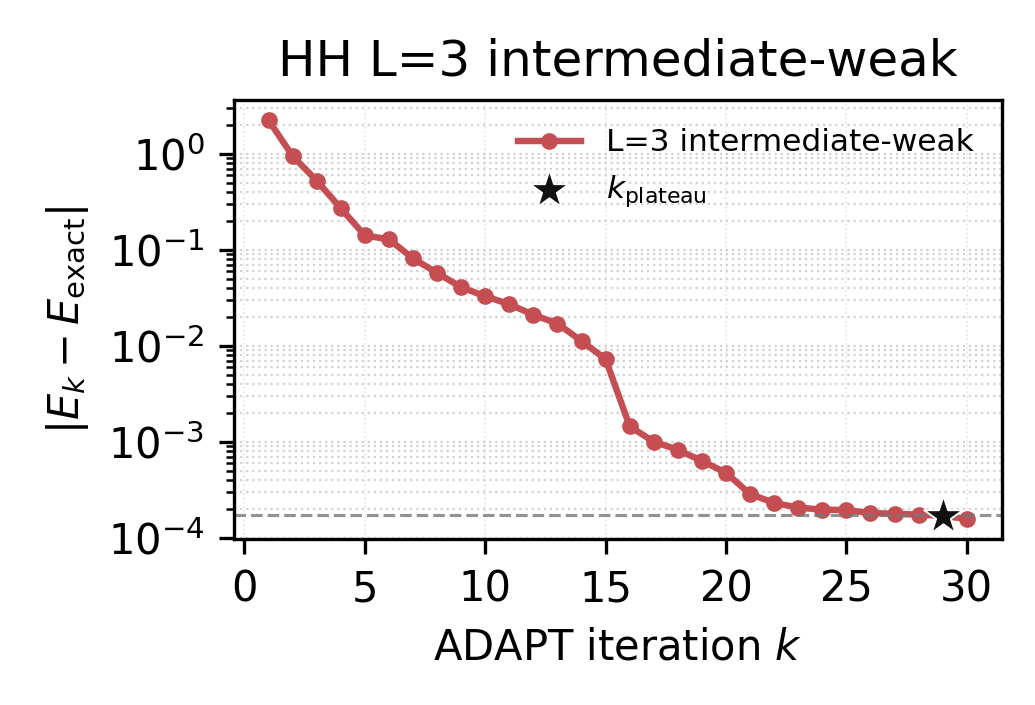
\includegraphics[width=\columnwidth]{figures/paper_i_hh_l3_intermediate_weak_physical_lanes_support_20260709/paper_i_hh_l3_intermediate_weak_error_vs_iteration_20260709.pdf}
\captionof{figure}{Three-site intermediate--weak Hubbard--Holstein SNAKE error versus ADAPT iteration for the physical-lane operator pool. The marker indicates the inferred plateau prefix \(k_{\rm pl}=29\).}
\label{fig:hh_l3_intermediate_weak_error_vs_iteration}
\end{center}

\begin{center}
\captionof{table}{\label{tab:hh_l3_intermediate_weak_plateau_costs}Three-site intermediate--weak Hubbard--Holstein SNAKE plateau-prefix Qiskit costs.}
\begin{tabular}{lrrrrrr}
\toprule
Method & \(k_{\rm pl}\) & \(|\Delta E|\) & \(N_{\twq}\) & \(D_{\twq}\) & \(D_c\) & \(S\) \\
\midrule
SNAKE & 29 & \(1.689\times10^{-4}\) & 122 & 98 & 488 & 44{,}467 \\
\bottomrule
\end{tabular}
\end{center}


\section{Spin-boson/Rabi benchmark}
\label{app:spin_boson_rabi}

The finite-mode spin-boson/Rabi benchmark is
\begin{equation*}
\begin{aligned}
H_{\rm SB}
&=-t_s\sigma_x+\Delta\sigma_z+\omega_0 b^\dagger b
+u_xX_b\sigma_x+g_zX_b\sigma_z,\\
X_b&=b^\dagger+b .
\end{aligned}
% source label: eq:spin_boson_rabi_appendix
\end{equation*}
Here \(\sigma_x,\sigma_y,\sigma_z\) are the Pauli matrices acting on the
two-level subsystem, and \(b^\dagger,b\) are truncated mode creation and
annihilation operators. The coefficient \(t_s\) sets the transverse two-level
term, \(\Delta\) is the longitudinal bias, \(\omega_0\) is the boson frequency,
and \(u_x\) and \(g_z\) are transverse and longitudinal quadrature-coupling
strengths. The conventional ultrastrong threshold is near
\(g/\omega_0\simeq 0.1\); the displayed rows use \(u_x=0\) and
\(g_z/\omega_0=0.05\) or \(0.1\) for the weak and stronger threshold-scale
points, respectively, with boson occupation cutoffs \(n_b^{\max}=1\) and
\(n_b^{\max}=2\) \cite{Kockum2019Ultrastrong,FornDiaz2019Ultrastrong}.

For the spin-boson/Rabi Hamiltonian, the operator pool combines two-level-system
rotations, bosonic quadrature response, nonlinear bosonic relaxation,
spin-conditioned bosonic response, and Hamiltonian-block channels. With
\(P_b=\ii(b^\dagger-b)\) and \(n_b=b^\dagger b\), the pool includes spin-only
channels, pure bosonic channels built from \(X_b\), \(P_b\), and \(n_b\),
spin-conditioned transverse channels such as \(X_b\sigma_x\), \(P_b\sigma_x\),
and \(n_b\sigma_x\), spin-conditioned longitudinal channels such as
\(X_b\sigma_z\), \(P_b\sigma_z\), and \(n_b\sigma_z\), nonlinear bosonic
channels such as \(\{n_b,P_b\}=n_bP_b+P_bn_b\) and \(X_bP_b+P_bX_b\), and
Hamiltonian-block channels. For the stronger cutoff case, the pool also
includes \(\sigma_y\)-conditioned correlation channels. SNAKE shortlists these
candidates through physical operator-type lanes separating two-level-system
motion, linear boson response, nonlinear boson response, transverse coupling,
longitudinal coupling, and Hamiltonian-block motion.

\noindent\begin{minipage}{0.49\columnwidth}
\begin{center}
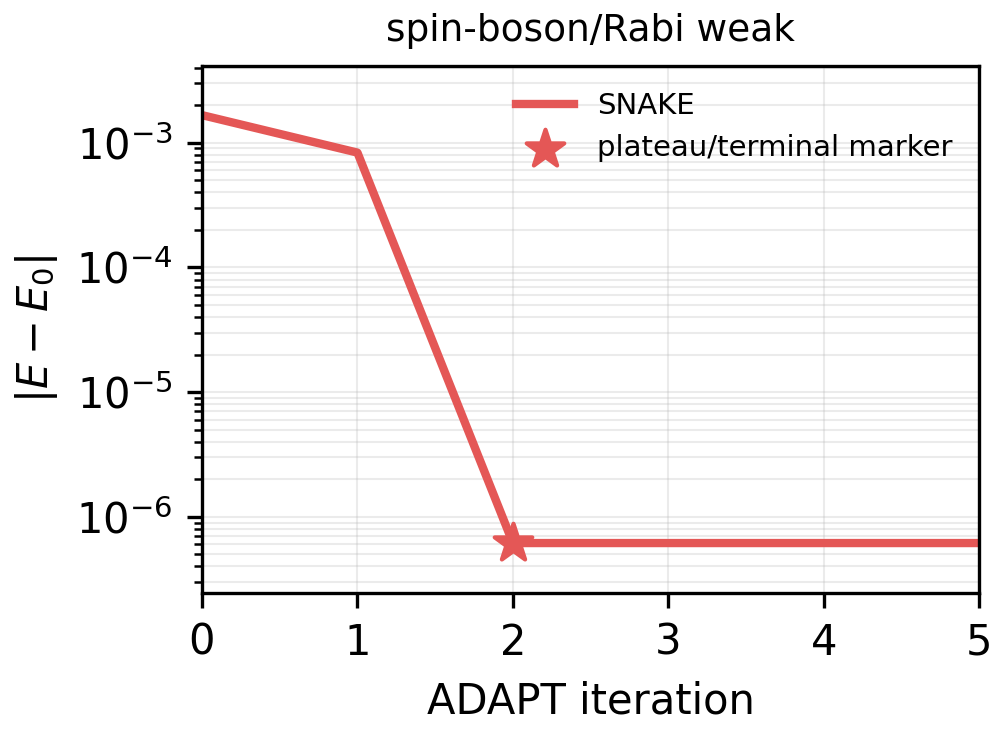
\includegraphics[width=\columnwidth]{figures/paper_i_alt_hamiltonian_1p75_20260709/paper_i_alt_snake_spin_boson_weak_error_vs_iteration.pdf}
\par\smallskip
\scriptsize
\textit{weak spin-boson/Rabi}
\par\smallskip
\setlength{\tabcolsep}{1.2pt}
\resizebox{\columnwidth}{!}{%
\begin{tabular}{@{}cccccc@{}}
\toprule
$k_{\rm pl}$ & $|\Delta E|$ & $N_{\twq}$ & $D_{\twq}$ & $D_c$ & $S$ \\
\midrule
2 & \(6{\times}10^{-7}\) & 19 & 17 & 123 & 685 \\
\bottomrule
\end{tabular}
}
\end{center}
\end{minipage}\hfill
\begin{minipage}{0.49\columnwidth}
\begin{center}
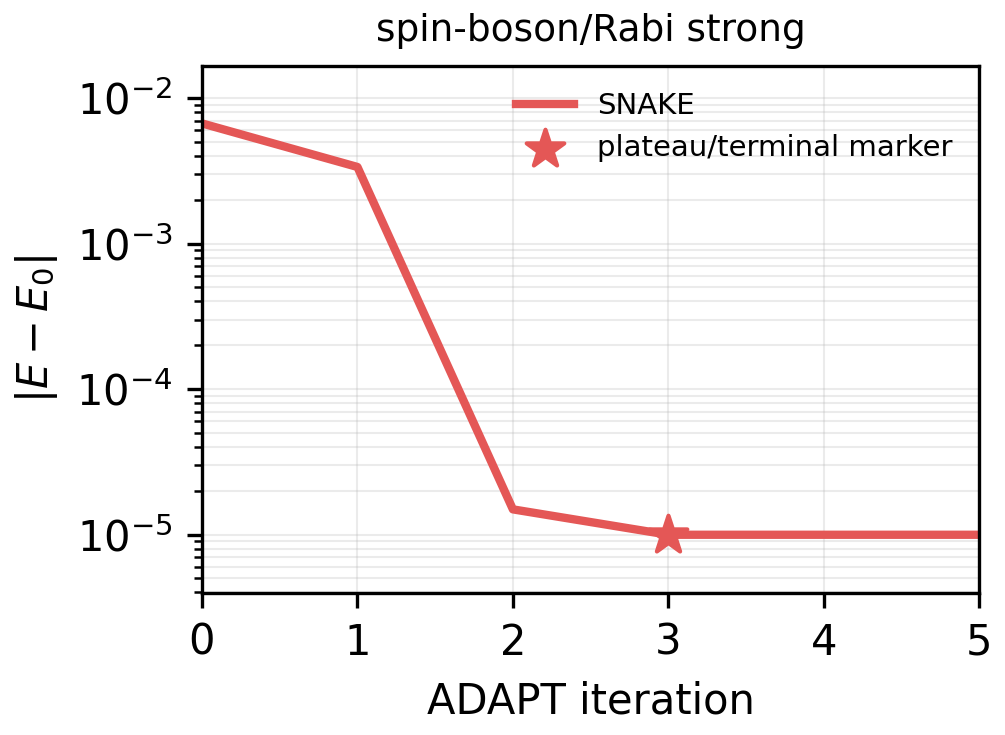
\includegraphics[width=\columnwidth]{figures/paper_i_alt_hamiltonian_1p75_20260709/paper_i_alt_snake_spin_boson_strong_error_vs_iteration.pdf}
\par\smallskip
\scriptsize
\textit{strong spin-boson/Rabi}
\par\smallskip
\setlength{\tabcolsep}{1.2pt}
\resizebox{\columnwidth}{!}{%
\begin{tabular}{@{}cccccc@{}}
\toprule
$k_{\rm pl}$ & $|\Delta E|$ & $N_{\twq}$ & $D_{\twq}$ & $D_c$ & $S$ \\
\midrule
3 & \(10{\times}10^{-6}\) & 115 & 111 & 723 & 3{,}754 \\
\bottomrule
\end{tabular}
}
\end{center}
\end{minipage}
\captionof{figure}{Spin-boson/Rabi SNAKE error versus ADAPT iteration and Qiskit plateau-prefix costs for weak and strong coupling.}
\par\addvspace{1.0ex}

\section{Bose--Hubbard benchmark}
\label{app:bose_hubbard}

For the Bose--Hubbard Hamiltonian, let \(b_i^\dagger,b_i\) be the bosonic
creation and annihilation operators on site \(i\). We define the local number
and quadrature operators
\[
n_i=b_i^\dagger b_i,\qquad
x_i=b_i+b_i^\dagger,\qquad
p_i=\ii(b_i^\dagger-b_i).
\]
The two-site open-boundary benchmark Hamiltonian is
\begin{equation*}
\begin{aligned}
H_{\rm BH}
&=-t\sum_{\langle i,j\rangle}
(b_i^\dagger b_j+b_j^\dagger b_i)
+\omega_0\sum_i n_i\\
&\quad+\frac{U_b}{2}\sum_i n_i(n_i-I)
+\Delta_v\sum_i(-1)^i n_i .
\end{aligned}
% source label: eq:bose_hubbard_appendix
\end{equation*}
Here \(t\) is the nearest-neighbor hopping amplitude, \(\omega_0\) is the
onsite boson energy, \(U_b\) is the onsite boson--boson interaction,
\(\Delta_v\) is the staggered onsite potential, \(I\) is the local identity,
and \(\langle i,j\rangle\) denotes nearest-neighbor sites. The displayed rows
use \(t=1\), \(\omega_0=1\), \(\Delta_v=0.25\), binary encoding with local
boson occupation cutoff \(n_b^{\max}=2\), and \(U_b=2\) or \(U_b=6\) for the
weak and strong interaction rows, respectively.
The operator pool is partitioned into physical operator-type lanes for number
and density interactions, onsite quadrature response, intersite quadrature
response, single-particle hopping/current, density-assisted transport, pair
transport, and Hamiltonian-block channels. These lanes include onsite number
operators \(n_i\), nonlinear number terms \(n_i^2\) and \(n_in_j\), onsite
quadratures \(x_i\), \(p_i\), \(x_i^2\), and \(p_i^2\), intersite quadratures
\(x_ix_j\) and \(p_ip_j\), hopping/current generators between sites,
density-weighted hopping/current generators, pair-hop/current generators, and
grouped Bose--Hubbard Hamiltonian blocks.

\noindent\begin{minipage}{0.49\columnwidth}
\begin{center}
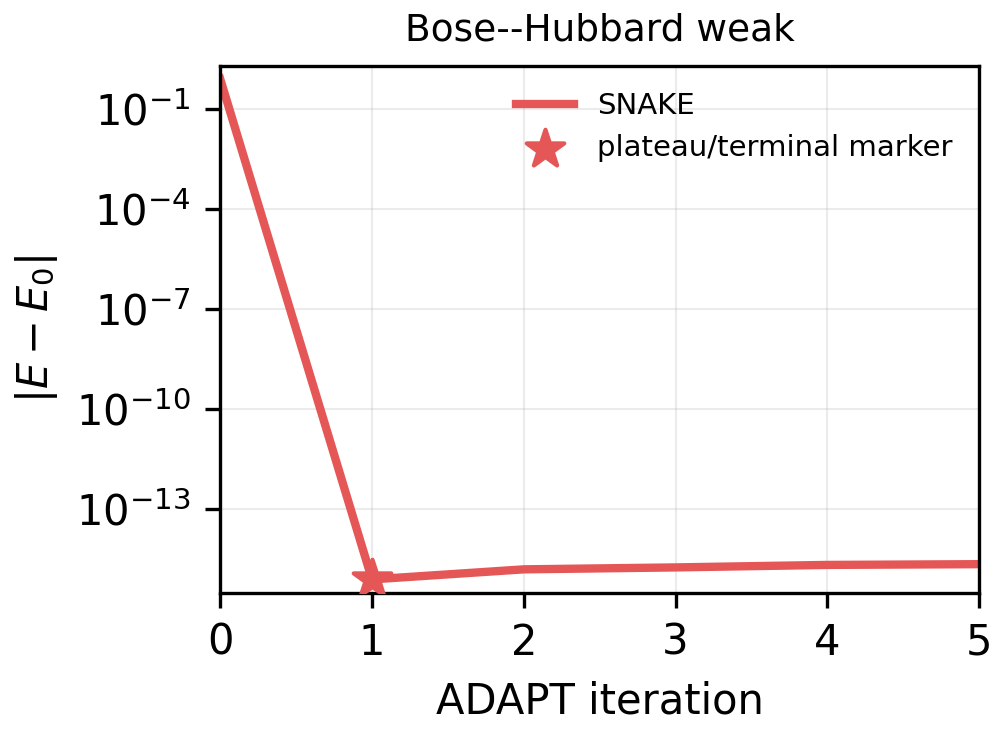
\includegraphics[width=\columnwidth]{figures/paper_i_alt_hamiltonian_1p75_20260709/paper_i_alt_snake_bose_hubbard_weak_error_vs_iteration.pdf}
\par\smallskip
\scriptsize
\textit{weak Bose--Hubbard}
\par\smallskip
\setlength{\tabcolsep}{1.2pt}
\resizebox{\columnwidth}{!}{%
\begin{tabular}{@{}cccccc@{}}
\toprule
$k_{\rm pl}$ & $|\Delta E|$ & $N_{\twq}$ & $D_{\twq}$ & $D_c$ & $S$ \\
\midrule
1 & \(8{\times}10^{-16}\) & 160 & 160 & 870 & 1{,}799 \\
\bottomrule
\end{tabular}
}
\end{center}
\end{minipage}\hfill
\begin{minipage}{0.49\columnwidth}
\begin{center}
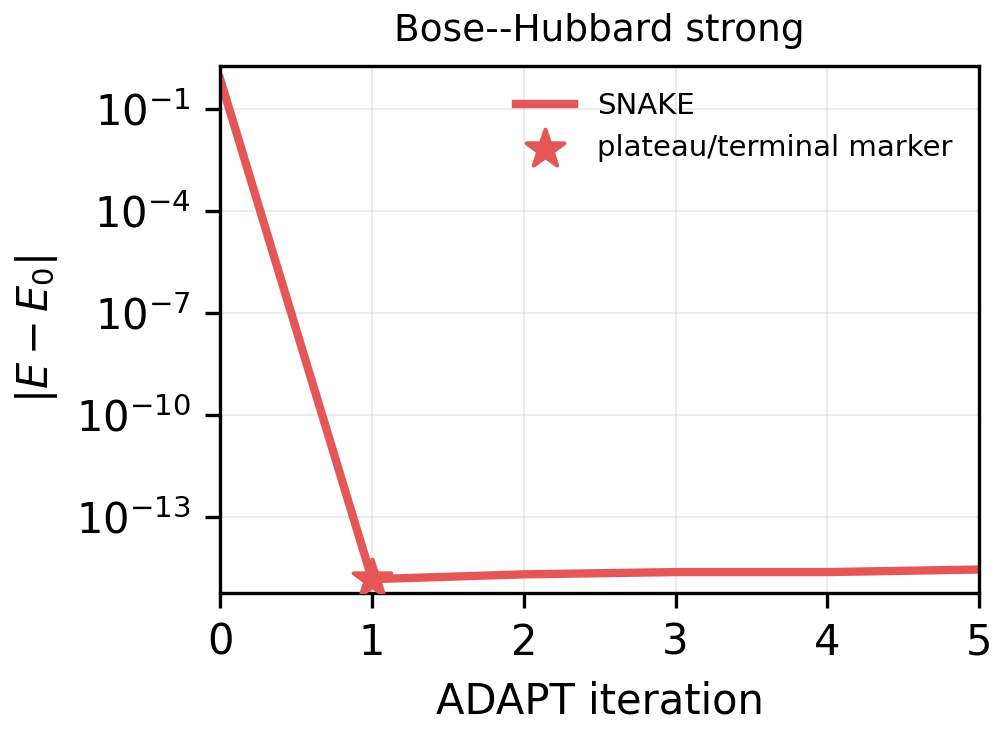
\includegraphics[width=\columnwidth]{figures/paper_i_alt_hamiltonian_1p75_20260709/paper_i_alt_snake_bose_hubbard_strong_error_vs_iteration.pdf}
\par\smallskip
\scriptsize
\textit{strong Bose--Hubbard}
\par\smallskip
\setlength{\tabcolsep}{1.2pt}
\resizebox{\columnwidth}{!}{%
\begin{tabular}{@{}cccccc@{}}
\toprule
$k_{\rm pl}$ & $|\Delta E|$ & $N_{\twq}$ & $D_{\twq}$ & $D_c$ & $S$ \\
\midrule
1 & \(1{\times}10^{-15}\) & 160 & 160 & 870 & 1{,}830 \\
\bottomrule
\end{tabular}
}
\end{center}
\end{minipage}
\captionof{figure}{Bose--Hubbard SNAKE error versus ADAPT iteration and Qiskit plateau-prefix costs for weak and strong interaction.}
\par\addvspace{1.0ex}

\section{Hubbard benchmarks}
\label{app:supplementary_transfer_benchmarks}

The Hubbard benchmark Hamiltonian is
\begin{equation*}
H_{\rm Hub}
=-t\sum_{\langle i,j\rangle,\sigma}
(c_{i\sigma}^{\dagger}c_{j\sigma}+c_{j\sigma}^{\dagger}c_{i\sigma})
+U\sum_i n_{i\uparrow}n_{i\downarrow}.
% source label: eq:hubbard_appendix
\end{equation*}
Here \(c_{i\sigma}^{\dagger},c_{i\sigma}\) are fermionic creation and
annihilation operators, \(n_{i\sigma}=c_{i\sigma}^{\dagger}c_{i\sigma}\),
\(\sigma\in\{\uparrow,\downarrow\}\), \(t\) is the nearest-neighbor hopping
amplitude, \(U\) is the onsite Hubbard interaction, and
\(\langle i,j\rangle\) denotes nearest-neighbor sites.
The displayed rows use a two-site open chain at half filling with \(t=1\).
For the Hubbard chain, the weak-coupling limit is given by
\(U/t\ll 1\), with correlation strength increasing as \(U/t\) grows;
we use \(U/t=0.25\) as a weak regime representative and \(U/t=8\) as the
strong-correlation point \cite{Arovas2022Hubbard}.

\noindent\begin{minipage}{0.49\columnwidth}
\begin{center}
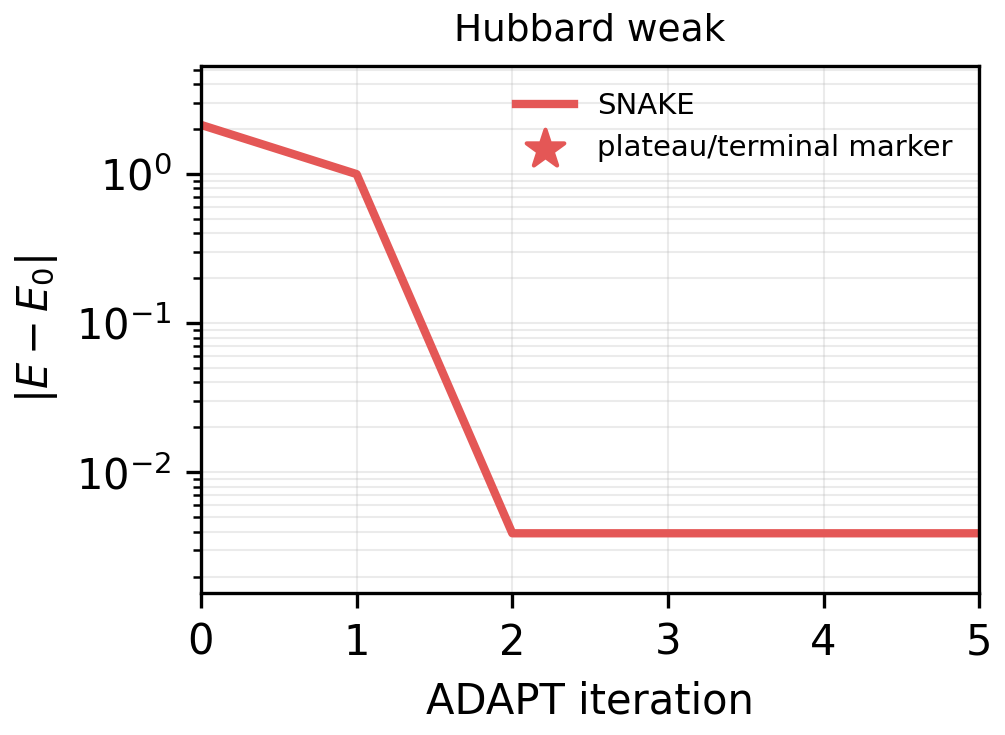
\includegraphics[width=\columnwidth]{figures/paper_i_alt_hamiltonian_1p75_20260709/paper_i_alt_snake_hubbard_weak_error_vs_iteration.pdf}
\par\smallskip
\scriptsize
\textit{weak Hubbard}
\par\smallskip
\setlength{\tabcolsep}{1.2pt}
\resizebox{\columnwidth}{!}{%
\begin{tabular}{@{}cccccc@{}}
\toprule
$k_{\rm pl}$ & $|\Delta E|$ & $N_{\twq}$ & $D_{\twq}$ & $D_c$ & $S$ \\
\midrule
8 & \(2{\times}10^{-11}\) & 18 & 10 & 120 & 5{,}936 \\
\bottomrule
\end{tabular}
}
\end{center}
\end{minipage}\hfill
\begin{minipage}{0.49\columnwidth}
\begin{center}
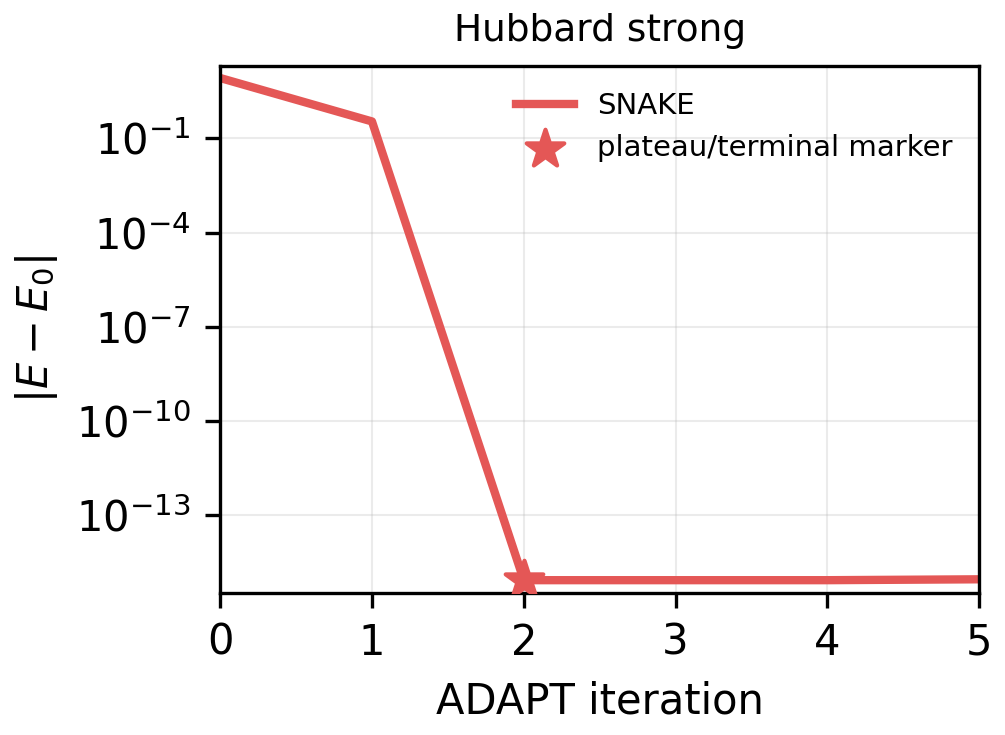
\includegraphics[width=\columnwidth]{figures/paper_i_alt_hamiltonian_1p75_20260709/paper_i_alt_snake_hubbard_strong_error_vs_iteration.pdf}
\par\smallskip
\scriptsize
\textit{strong Hubbard}
\par\smallskip
\setlength{\tabcolsep}{1.2pt}
\resizebox{\columnwidth}{!}{%
\begin{tabular}{@{}cccccc@{}}
\toprule
$k_{\rm pl}$ & $|\Delta E|$ & $N_{\twq}$ & $D_{\twq}$ & $D_c$ & $S$ \\
\midrule
2 & \(8{\times}10^{-16}\) & 52 & 52 & 274 & 751 \\
\bottomrule
\end{tabular}
}
\end{center}
\end{minipage}
\captionof{figure}{Hubbard SNAKE error versus ADAPT iteration and Qiskit plateau-prefix costs for weak and strong interaction.}
\par\addvspace{1.0ex}

\section{SPSA optimizer settings and sensitivity}
\label{app:spsa_settings}

SPSA-based diagnostic and comparator records use simultaneous perturbation
stochastic approximation as the inner optimizer
\cite{Spall1992SPSA,Kandala2017}. This optimizer appendix is separated from
the SNAKE algorithmic settings because SPSA is an inner-refit convention, not a
shortlisting, batching, insertion, or ablation rule.

At SPSA optimizer step \(m\), with Rademacher perturbation vector
\(\Delta_m\), the two-evaluation gradient estimator and parameter update are
\begin{align*}
a_m&=\frac{a}{(A+m+1)^\alpha},\qquad
c_m=\frac{c}{(m+1)^\gamma}, \nonumber\\
E_m^\pm&=E(\boldsymbol{\theta}_m\pm c_m\Delta_m), \nonumber\\
(\widehat g_m)_i&=\frac{E_m^+-E_m^-}{2c_m(\Delta_m)_i}, \nonumber\\
\boldsymbol{\theta}_{m+1}&=\boldsymbol{\theta}_m-a_m\widehat{\mathbf g}_m .
% source label: eq:spsa_inner_optimizer
\end{align*}
The schedule family uses \(m_{\max}=200\) unless a diagnostic row states a
larger budget. The realized Hubbard--Holstein schedule parameters are as
follows; ranges denote the minimum and maximum over the six regimes.
\begin{center}
\scriptsize
\setlength{\tabcolsep}{1.4pt}
\renewcommand{\arraystretch}{1.05}
\begin{tabular}{lcccccc}
Method & \(m_{\max}\) & \(a\) & \(c\) & \(A\) & \(\alpha\) & \(\gamma\)\\
Append & 200 & 0.0195--0.0454 & 0.00502--0.0118 & 12.4--59.0 & 0.602 & 0.101\\
Geo & 200 & 0.0169--0.0741 & 0.00501--0.0368 & 13.2--86.5 & 0.602 & 0.101\\
SNAKE & 200 & 0.100 & 0.020 & 5.0 & 0.602 & 0.101\\
\end{tabular}
\end{center}

\clearpage
\begin{thebibliography}{99}

\bibitem{Hubbard1963}
J. Hubbard,
``Electron correlations in narrow energy bands,''
\emph{Proceedings of the Royal Society of London A} \textbf{276}, 238 (1963).

\bibitem{Holstein1959a}
T. Holstein,
``Studies of polaron motion: Part I. The molecular-crystal model,''
\emph{Annals of Physics} \textbf{8}, 325 (1959).

\bibitem{Holstein1959b}
T. Holstein,
``Studies of polaron motion: Part II. The small polaron,''
\emph{Annals of Physics} \textbf{8}, 343 (1959).

\bibitem{Sakkinen2015HolsteinDimer}
N. S\"akkinen, Y. Peng, H. Appel, and R. van Leeuwen,
``Many-body Green's function theory for electron-phonon interactions: Ground state properties of the Holstein dimer,''
\emph{Journal of Chemical Physics} \textbf{143}, 234101 (2015).

\bibitem{Dorfner2015HolsteinDecay}
F. Dorfner, L. Vidmar, C. Brockt, E. Jeckelmann, and F. Heidrich-Meisner,
``Real-time decay of a highly excited charge carrier in the one-dimensional Holstein model,''
\emph{Physical Review B} \textbf{91}, 104302 (2015).

\bibitem{tenBrink2022HolsteinDynamics}
M. ten Brink, S. Gr\"aber, M. Hopjan, D. Jansen, J. Stolpp, F. Heidrich-Meisner, and P.~E. Bl\"ochl,
``Real-time non-adiabatic dynamics in the one-dimensional Holstein model: Trajectory-based vs exact methods,''
\emph{Journal of Chemical Physics} \textbf{156}, 234109 (2022).

\bibitem{Cataudella1999HolsteinVariational}
V. Cataudella, G. De Filippis, and G. Iadonisi,
``A new variational approach for the Holstein molecular-crystal model,''
\emph{Physical Review B} \textbf{60}, 15163 (1999).

\bibitem{ClayHardikar2005HH}
R.~T. Clay and R.~P. Hardikar,
``Intermediate phase of the one-dimensional half-filled Hubbard-Holstein model,''
\emph{Physical Review Letters} \textbf{95}, 096401 (2005).

\bibitem{Tezuka2007HH}
A. Tezuka, R. Arita, and H. Aoki,
``Phase diagram for the one-dimensional Hubbard-Holstein model: a density-matrix renormalization group study,''
\emph{Physical Review B} \textbf{76}, 155114 (2007).

\bibitem{Weisse2008}
A. Wei{\ss}e and H. Fehske,
``Exact diagonalization techniques,''
in \emph{Computational Many-Particle Physics},
edited by H. Fehske, R. Schneider, and A. Wei{\ss}e,
Lecture Notes in Physics Vol. 739 (Springer, Berlin, Heidelberg, 2008), pp. 529--544.

\bibitem{Troyer2005}
M. Troyer and U.-J. Wiese,
``Computational complexity and fundamental limitations to fermionic quantum Monte Carlo simulations,''
\emph{Physical Review Letters} \textbf{94}, 170201 (2005).

\bibitem{Schollwock2011}
U. Schollw\"ock,
``The density-matrix renormalization group in the age of matrix product states,''
\emph{Annals of Physics} \textbf{326}, 96 (2011).

\bibitem{Arovas2022Hubbard}
D.~P. Arovas, E. Berg, S.~A. Kivelson, and S. Raghu,
``The Hubbard model,''
\emph{Annual Review of Condensed Matter Physics} \textbf{13}, 239--274 (2022).

\bibitem{LeBlanc2015HubbardBenchmarks}
J.~P.~F. LeBlanc et al.,
``Solutions of the two-dimensional Hubbard model: Benchmarks and results from a wide range of numerical algorithms,''
\emph{Physical Review X} \textbf{5}, 041041 (2015).

\bibitem{Qin2016AFQMCHubbard}
M. Qin, H. Shi, and S. Zhang,
``Benchmark study of the two-dimensional Hubbard model with auxiliary-field quantum Monte Carlo method,''
\emph{Physical Review B} \textbf{94}, 085103 (2016).

\bibitem{Alvertis2024HubbardVQE}
K. Alvertis et al.,
``Classical Benchmarks for Variational Quantum Eigensolver Simulations of the Hubbard Model,''
\emph{arXiv:2408.00836} (2024).

\bibitem{Lloyd1996}
S. Lloyd,
``Universal quantum simulators,''
\emph{Science} \textbf{273}, 1073--1078 (1996).

\bibitem{AspuruGuzik2005}
A. Aspuru-Guzik, A.~D. Dutoi, P.~J. Love, and M. Head-Gordon,
``Simulated quantum computation of molecular energies,''
\emph{Science} \textbf{309}, 1704--1707 (2005).

\bibitem{Preskill2018NISQ}
J. Preskill,
``Quantum computing in the NISQ era and beyond,''
\emph{Quantum} \textbf{2}, 79 (2018).

\bibitem{Huggins2021Measurements}
W.~J. Huggins, J.~R. McClean, N.~C. Rubin, Z. Jiang, N. Wiebe, K.~B. Whaley, and R. Babbush,
``Efficient and noise resilient measurements for quantum chemistry on near-term quantum computers,''
\emph{npj Quantum Information} \textbf{7}, 23 (2021).

\bibitem{Romero2018UCC}
J. Romero, R. Babbush, J.~R. McClean, C. Hempel, P.~J. Love, and A. Aspuru-Guzik,
``Strategies for quantum computing molecular energies using the unitary coupled cluster ansatz,''
\emph{Quantum Science and Technology} \textbf{4}, 014008 (2018).

\bibitem{Peruzzo2014}
A. Peruzzo, J. McClean, P. Shadbolt, M.-H. Yung, X.-Q. Zhou, P.~J. Love, A. Aspuru-Guzik, and J.~L. O'Brien,
``A variational eigenvalue solver on a photonic quantum processor,''
\emph{Nature Communications} \textbf{5}, 4213 (2014).

\bibitem{McClean2016}
J.~R. McClean, J. Romero, R. Babbush, and A. Aspuru-Guzik,
``The theory of variational hybrid quantum-classical algorithms,''
\emph{New Journal of Physics} \textbf{18}, 023023 (2016).

\bibitem{Kandala2017}
A. Kandala, A. Mezzacapo, K. Temme, M. Takita, M. Brink, J.~M. Chow, and J.~M. Gambetta,
``Hardware-efficient variational quantum eigensolver for small molecules and quantum magnets,''
\emph{Nature} \textbf{549}, 242 (2017).

\bibitem{Cerezo2021VQA}
M. Cerezo, A. Arrasmith, R. Babbush, S.~C. Benjamin, S. Endo, K. Fujii, J.~R. McClean, K. Mitarai, X. Yuan, L. Cincio, and P.~J. Coles,
``Variational quantum algorithms,''
\emph{Nature Reviews Physics} \textbf{3}, 625--644 (2021).

\bibitem{VanStraaten2021MeasurementCost}
B. van Straaten and B. Koczor,
``Measurement cost of metric-aware variational quantum algorithms,''
\emph{PRX Quantum} \textbf{2}, 030324 (2021).

\bibitem{Spall1992SPSA}
J.~C. Spall,
``Multivariate stochastic approximation using a simultaneous perturbation gradient approximation,''
\emph{IEEE Transactions on Automatic Control} \textbf{37}, 332--341 (1992).

\bibitem{BonetMonroig2023Optimizer}
X. Bonet-Monroig, H. Wang, D. Vermetten, B. Senjean, C. Moussa, T. B\"ack, V. Dunjko, and T.~E. O'Brien,
``Performance comparison of optimization methods on variational quantum algorithms,''
\emph{Physical Review A} \textbf{107}, 032407 (2023).

\bibitem{Singh2023Optimizers}
H. Singh, S. Mishra, and S. Majumder,
``Benchmarking of different optimizers in the variational quantum algorithms for applications in quantum chemistry,''
\emph{Journal of Chemical Physics} \textbf{159}, 044117 (2023).

\bibitem{Jones2025FermiHubbardOptimizers}
B.~D.~M. Jones, L. Mineh, and A. Montanaro,
``Benchmarking a wide range of optimisers for solving the Fermi-Hubbard model using the variational quantum eigensolver,''
\emph{arXiv:2411.13742} (2025).

\bibitem{McClean2018BarrenPlateaus}
J.~R. McClean, S. Boixo, V.~N. Smelyanskiy, R. Babbush, and H. Neven,
``Barren plateaus in quantum neural network training landscapes,''
\emph{Nature Communications} \textbf{9}, 4812 (2018).

\bibitem{LiBenjamin2017VQS}
Y. Li and S.~C. Benjamin,
``Efficient variational quantum simulator incorporating active error minimization,''
\emph{Physical Review X} \textbf{7}, 021050 (2017).

\bibitem{Yuan2019VQS}
X. Yuan, S. Endo, Q. Zhao, Y. Li, and S.~C. Benjamin,
``Theory of variational quantum simulation,''
\emph{Quantum} \textbf{3}, 191 (2019).

\bibitem{McClean2017QSE}
J.~R. McClean, M.~E. Kimchi-Schwartz, J. Carter, and W.~A. de Jong,
``Hybrid quantum-classical hierarchy for mitigation of decoherence and determination of excited states,''
\emph{Physical Review A} \textbf{95}, 042308 (2017).

\bibitem{Grimsley2019}
H.~R. Grimsley, S.~E. Economou, E. Barnes, and N.~J. Mayhall,
``An adaptive variational algorithm for exact molecular simulations on a quantum computer,''
\emph{Nature Communications} \textbf{10}, 3007 (2019).

\bibitem{Grimsley2023ADAPT}
H.~R. Grimsley, G.~S. Barron, E. Barnes, S.~E. Economou, and N.~J. Mayhall,
``Adaptive, problem-tailored variational quantum eigensolver mitigates rough parameter landscapes and barren plateaus,''
\emph{npj Quantum Information} \textbf{9}, 19 (2023).

\bibitem{Tang2021}
H.~L. Tang, V.~O. Shkolnikov, G.~S. Barron, H.~R. Grimsley, N.~J. Mayhall, E. Barnes, and S.~E. Economou,
``Qubit-ADAPT-VQE: An adaptive algorithm for constructing hardware-efficient ans\"atze on a quantum processor,''
\emph{PRX Quantum} \textbf{2}, 020310 (2021).

\bibitem{Yordanov2021}
Y.~S. Yordanov, V. Armaos, C.~H.~W. Barnes, and D.~R.~M. Arvidsson-Shukur,
``Qubit-excitation-based adaptive variational quantum eigensolver,''
\emph{Communications Physics} \textbf{4}, 228 (2021).

\bibitem{Feniou2023}
C. Feniou, M. Hassan, D. Traor\'e, E. Giner, Y. Maday, and J.-P. Piquemal,
``Overlap-ADAPT-VQE: Practical quantum chemistry on quantum computers via overlap-guided compact ans\"atze,''
\emph{Communications Physics} \textbf{6}, 192 (2023).

\bibitem{Majland2024vADAPT}
M. Majland, P. Ettenhuber, N.~T. Zinner, and O. Christiansen,
``Vibrational ADAPT-VQE: Critical points lead to problematic convergence,''
\emph{Journal of Chemical Physics} \textbf{160}, 154109 (2024).

\bibitem{Anastasiou2024}
P.~G. Anastasiou, Y. Chen, N.~J. Mayhall, E. Barnes, and S.~E. Economou,
``TETRIS-ADAPT-VQE: An adaptive algorithm that yields shallower, denser circuit ans\"atze,''
\emph{Physical Review Research} \textbf{6}, 013254 (2024).

\bibitem{Ramoa2025}
M. Ram\^oa, P.~G. Anastasiou, L.~P. Santos, N.~J. Mayhall, E. Barnes, and S.~E. Economou,
``Reducing the resources required by ADAPT-VQE using coupled exchange operators and improved subroutines,''
\emph{npj Quantum Information} \textbf{11}, 86 (2025).

\bibitem{Ramoa2025HessianRecycling}
M. Ramoa et al.,
``Reducing measurement costs by recycling the Hessian in adaptive variational quantum algorithms,''
\emph{Quantum Science and Technology} \textbf{10}, 015031 (2025).

\bibitem{He2026ParamADAPT}
R. He, X. Hong, Q. Chai, J. Guan, J. Zhou, A. Ablimit, G. Cui, and S. Ying,
``Constructing Compact ADAPT Unitary Coupled-Cluster Ansatz with Parameter-Based Criterion,''
\emph{Journal of Chemical Theory and Computation} \textbf{22}, 5090--5101 (2026).

\bibitem{He2026HAADAPT}
R. He, C. Liu, X. Hong, Q. Chai, J. Zhou, J. Guan, G. Cui, and S. Ying,
``Hamiltonian-Aware ADAPT Variational Quantum Eigensolver for Molecular Ground-State Simulation,''
\emph{arXiv:2606.13118} (2026).

\bibitem{Bespalova2026KADAPT}
T.~A. Bespalova, O. Ladhari, and G. Masella,
``K-ADAPT-VQE: Optimizing Molecular Ground State Searches by Chunking Operators,''
in \emph{Quantum Engineering Sciences and Technologies for Industry and Services}, Communications in Computer and Information Science \textbf{2744}, 226--235 (Springer, Cham, 2026).

\bibitem{Nocedal2006TrustRegion}
J. Nocedal and S. J. Wright,
``Trust-Region Methods,''
in \emph{Numerical Optimization}, Springer (New York, NY, 1994).

\bibitem{IglewiczHoaglin1993}
B. Iglewicz and D.~C. Hoaglin,
\emph{How to Detect and Handle Outliers},
ASQC Basic References in Quality Control: Statistical Techniques, Vol.~16
(ASQC Quality Press, Milwaukee, WI, 1993).

\bibitem{Burbidge1988IHS}
J.~B. Burbidge, L. Magee, and A.~L. Robb,
``Alternative transformations to handle extreme values of the dependent variable,''
\emph{Journal of the American Statistical Association} \textbf{83}, 123--127 (1988).

\bibitem{Ikhtiarudin2025ShotEfficient}
A. Ikhtiarudin, G. K. Sunnardianto, F. Fathurrahman, M. K. Agusta, and H. Dipojono,
``Shot-Efficient ADAPT-VQE via Reused Pauli Measurements and Variance-Based Shot Allocation,''
\emph{arXiv:2507.16879} (2025).

\bibitem{Lowerre1976Beam}
B. T. Lowerre,
``The Harpy Speech Recognition System,''
Ph.D. thesis, Carnegie Mellon University (1976).

\bibitem{Sohail2026GeoADAPT}
M.~A. Sohail and T. Koike-Akino,
``Geo-ADAPT-VQE: Quantum Information Metric-Aware Circuit Optimization for Quantum Chemistry,''
\emph{arXiv:2603.10325} (2026).

\bibitem{Stadelmann2025GradientTroughs}
T. Stadelmann and others,
``Strategies for overcoming gradient troughs in the ADAPT-VQE algorithm,''
\emph{arXiv:2512.25004} (2025).

\bibitem{ProvostVallee1980}
J.-P. Provost and G. Vall\'ee,
``Riemannian structure on manifolds of quantum states,''
\emph{Communications in Mathematical Physics} \textbf{76}, 289 (1980).

\bibitem{Stokes2020QNG}
J. Stokes, J. Izaac, N. Killoran, and G. Carleo,
``Quantum natural gradient,''
\emph{Quantum} \textbf{4}, 269 (2020).

\bibitem{Haug2021Capacity}
T. Haug, K. Bharti, and M.~S. Kim,
``Capacity and quantum geometry of parametrized quantum circuits,''
\emph{PRX Quantum} \textbf{2}, 040309 (2021).

\bibitem{Gacon2021QNSPSA}
J. Gacon, C. Zoufal, G. Carleo, and S. Woerner,
``Simultaneous perturbation stochastic approximation of the quantum Fisher information,''
\emph{Quantum} \textbf{5}, 567 (2021).

\bibitem{JavadiAbhari2024Qiskit}
A. Javadi-Abhari, M. Treinish, K. Krsulich, C.~J. Wood, J. Lishman, J. Gacon, S. Martiel, P.~D. Nation, L.~S. Bishop, A.~W. Cross, B.~R. Johnson, and J.~M. Gambetta,
``Quantum computing with Qiskit,''
\emph{arXiv:2405.08810} (2024).

\bibitem{QiskitAlgorithmsAdaptVQE}
Qiskit Community,
``AdaptVQE,''
\emph{Qiskit Algorithms documentation}, \url{https://qiskit-community.github.io/qiskit-algorithms/stubs/qiskit_algorithms.AdaptVQE.html}.

\bibitem{Larocca2023Overparametrization}
M. Larocca, N. Ju, D. Garc{\'i}a-Mart{\'i}n, P.~J. Coles, and M. Cerezo,
``Theory of overparametrization in quantum neural networks,''
\emph{Nature Computational Science} \textbf{3}, 542--551 (2023).

\bibitem{Verteletskyi2020CliqueCover}
V. Verteletskyi, T.-C. Yen, and A.~F. Izmaylov,
``Measurement optimization in the variational quantum eigensolver using a minimum clique cover,''
\emph{Journal of Chemical Physics} \textbf{152}, 124114 (2020).

\bibitem{Yen2020CompatibleMeasurements}
T.-C. Yen, V. Verteletskyi, and A.~F. Izmaylov,
``Measuring all compatible operators in one series of single-qubit measurements using unitary transformations,''
\emph{Journal of Chemical Theory and Computation} \textbf{16}, 2400 (2020).


\bibitem{Macridin2018}
A. Macridin, P. Spentzouris, J. Amundson, and R. Harnik,
``Electron-phonon systems on a universal quantum computer,''
\emph{Physical Review Letters} \textbf{121}, 110504 (2018).

\bibitem{Sawaya2020}
N.~P.~D. Sawaya, T. Menke, T.~H. Kyaw, S. Johri, A. Aspuru-Guzik, and G.~G. Guerreschi,
``Resource-efficient digital quantum simulation of $d$-level systems for photonic, vibrational, and spin-$s$ Hamiltonians,''
\emph{npj Quantum Information} \textbf{6}, 49 (2020).

\bibitem{Li2023}
W. Li, J. Ren, S. Huai, T. Cai, Z. Shuai, and S. Zhang,
``Efficient quantum simulation of electron-phonon systems by variational basis state encoder,''
\emph{Physical Review Research} \textbf{5}, 023046 (2023).

\bibitem{Denner2023}
M.~M. Denner, H. Yan, N. A. Sinitsyn, and others,
``A hybrid quantum-classical method for electron-phonon systems,''
\emph{Communications Physics} \textbf{6}, 317 (2023).

\bibitem{Dutta2024BosonicChemistry}
R. Dutta et al.,
``Simulating chemistry on bosonic quantum devices,''
\emph{Journal of Chemical Theory and Computation} \textbf{20}, 6426--6441 (2024).

\bibitem{Dutta2026QumodeVQE}
R. Dutta, C. Cianci, A.~V. Soudackov, Y. Wang, C. Xu, D. Mazziotti, L.~F. Santos, and V.~S. Batista,
``Qumode-Based Variational Quantum Eigensolver for Molecular Excited States,''
\emph{Journal of Chemical Theory and Computation} \textbf{22}, 993--1003 (2026).

\bibitem{Rinaldi2022MatrixModels}
E. Rinaldi, X. Han, M. Hassan, Y. Feng, F. Nori, M. McGuigan, and M. Hanada,
``Matrix-Model Simulations Using Quantum Computing, Deep Learning, and Lattice Monte Carlo,''
\emph{PRX Quantum} \textbf{3}, 010324 (2022).

\bibitem{Dao2025SU2MatrixVQE}
H.~L. Dao,
``Exploring new variational quantum circuit ansatzes for solving SU(2) matrix models,''
\emph{European Physical Journal C} \textbf{85}, 705 (2025).

\bibitem{Peng2025BosonHamiltonians}
B. Peng, Y. Su, D. Claudino, K. Kowalski, G. H. Low, and M. Roetteler,
``Quantum simulation of boson-related Hamiltonians: Techniques, effective Hamiltonian construction, and error analysis,''
\emph{Quantum Science and Technology} \textbf{10}, 023002 (2025).

\bibitem{Kockum2019Ultrastrong}
A.~F. Kockum, A. Miranowicz, S. De Liberato, S. Savasta, and F. Nori,
``Ultrastrong coupling between light and matter,''
\emph{Nature Reviews Physics} \textbf{1}, 19--40 (2019).

\bibitem{FornDiaz2019Ultrastrong}
P. Forn-D{\'i}az, L. Lamata, E. Rico, J. Kono, and E. Solano,
``Ultrastrong coupling regimes of light-matter interaction,''
\emph{Reviews of Modern Physics} \textbf{91}, 025005 (2019).

\bibitem{Vaquero2025PrunedADAPT}
N. Vaquero-Sabater, A. Carreras, and D. Casanova,
``Pruned-ADAPT-VQE: Compacting Molecular Ans\"atze by Removing Irrelevant Operators,''
\emph{Journal of Chemical Theory and Computation} \textbf{21}, 8720--8728 (2025).

\end{thebibliography}

\end{document}
